%% !TeX program = lualatex

%\listfiles	
% **************************
% STOP - Bitte zuerst lesen, bevor Sie weitermachen
%
% Einige Dinge müssen Sie an Ihre Bedürfnisse (und die Vorgaben Ihres
% Betreuers anpassen. Editieren Sie dazu die Datei docinfo.tex).
%
% 1. Sprache
% Das Template unterstützt Deutsch und Englisch, Standard ist Deutsch.
% Wenn Sie Englisch verwenden wollen, ändern Sie bitte direkt am Anfang
% dieser Datei den Eintrag
%    \newcommand{\hsmasprache}{de}
% auf
%    \newcommand{\hsmasprache}{en}
%
% 2. Form der Abgabe
% Das Template unterstützt sowohl eine digitale Abgabe, als auch eine Abgabe
% auf Papier. Bei einer Papierabgabe wird ein doppelseitiger Druck vorbereitet
% und der Titel wird so platziert, dass er in das Fenster des offiziellen
% Umschlages der Technischen Hochschule passt.
% Bei einer digitalen Abgabe (als PDF) wird der Titel zentriert und als
% Format wird einseitig gewählt. Außerdem wird die Datei unterschrift.png
% auf dem Blatt mit der Erklärung zur Eigenständigkeit eingebunden.
%
% 3. Zitierstil
% Abhängig von dem gewünschten Zitierstil passen Sie bitte in
% hma.cls die Einstellungen bei \RequirePackage[backend=biber...
% an. Wie ist dort genau erklärt.
% Achtung: Wenn Sie als Zitierstil Fußnoten wählen bzw. generell
% -------  mit Fußnoten arbeiten, dann beachten Sie bitte, dass
%          Fußnoten in Bildunterschriften und Tabellenüberschriften
%          nicht funktionieren.
%          Siehe hierzu https://texfaq.org/FAQ-ftncapt
%          und https://texfaq.org/FAQ-footintab
%          Sinnvollerweise verzichten Sie auf Fußnoten an diesen
%          Stellen und fügen Quellen einfach per \parancite ein.
%
% 4. Doppelseitiger oder einseitiger Druck
% Das Template bestimmt, ob einseitig oder doppelseitig gedruckt wird
% anhand der Abgabeform (papier / digital). Wollen sie dies übersteuern,
% müssen Sie in der Datei preambel.tex folgende Zeile
% \KOMAoptions{twoside=true} für doppelsetigen Druck
% \KOMAoptions{twoside=false} für einsetigen Druck
% direkt vor \usepackage{xcolor} einsetzen. Prinzipiell sollten Sie aber
% das vorgeschlagene Format einfach so lassen.
%
% 5. Unnötige Teile entfernen
% Entfernen Sie die Teile, die Sie nicht brauchen, z.B. Anhänge
%
% 6. Silbentrennung
% LaTeX führt eine automatische Silbentrennung durch. Allerdings
% werden Wörter, die bereits einen Bindestrich enthalten nicht
% getrennt, z.B. Datenschutz-Grundverordnung. Wenn Sie Ihren Text auf
% Deutsch schreiben, können Sie dann alternativ "= für den Bindestrich
% im Wort verwenden, z.B. Datenschutz"=Grundverordnung, damit LaTeX
% weiterhin richtig trennt.
% Ist die Silbentrennung aus einem anderen Grund nicht erfolgt, sodass
% das Wort über den rechten Rand hinaussteht oder wenn Sie eine weitere
% Trennstelle wollen, können Sie LaTeX helfen, indem Sie weitere
% Trennstellen angeben. Dies geschieht durch "- als Zeichen, z.B.
% Staats"-vertrag.
%
% 7. Nummerierung der Fußnoten
% LaTeX beginnt die Nummerierung der Fußnoten in jedem Kapitel wieder
% bei 1. In diesem Template wird die fortlaufende Nummerierung der Fußnoten 
% über die gesamte Arbeit umgesetzt.  
%
% 8. Unterschrift
% Bei einer Abgabe auf Papier unterschreiben Sie die Arbeit eigenhändig.
% Geben Sie allerdings digital ab, sollten Sie die Datei unterschrift.png in dem 
% Ordner /bilder durch einen Scan Ihrer eigenen Unteschrift ersetzen - andernfalls
% unterschreiben Sie als Max Mustermann ;-)
% *******************************************************************


% Dokumenteneinstellungen und Infos importieren
% -------------------------------------------------------
% Informationen und Einstellungen für Ihre Abschlussarbeit
%

% Sprache für das Dokument festlegen
\newcommand{\hsmasprache}{de} %de für Deutsch oder en für Englisch


% Abgabeform festlegen
% Bei einer digitalen Abgabe, wird das Dokument einseitig erzeugt und der Titel wird
% zentriert.
\newcommand{\hsmaabgabe}{digital} % Abgabe erfolgt für Fakultät I digital. Optionen hier sind für anderen Fakultäten: "papier" oder "digital".


% Flags für Veröffentlichung, Sperrvermerk
\newcommand{\hsmapublizieren}{opensource}   
% Wird einer Veröffentlichung zugestimmt?
% Optionen: 
% opensource = Druck der CC Lizenz mit By SA (Standard)
% hs = Veröffentlichung an der Technischen Hochschule und auf Hochschulservern
% stud = kein opensource und keine veröffentlichung auf den Hochschulservern
% vertraulich = Arbeit darf nicht veröffentlicht werden und erhält einen Sperrvermerk (Nur nach Absprache mit Betreuer setzen!)


\newcommand{\genderhinweis}{gender}     % Soll der Gender-Hinweis angezeigt werden? ja=gender, nein = nogender; Genderhinweis wird nur in deutscher Sprache angezeigt!


\newcommand{\hsmaquellcode}{sourcecode} % Verwenden Sie Quellcode in Ihrer Arbeit? ja=sourcecode, nein= nosourcecode

\newcommand{\hsmasymbole}{symbole} % Verwenden Sie viele Symbole in Ihrer Arbeit, welche in einem Symbolverzeichnis aufgeführt werden sollen? ja=symbole, nein= nosymbole


\newcommand{\hsmaglossar}{glossar} % Verwenden Sie Begriffserklärungen nicht Abkürzungen in Ihrer Arbeit? ja=glossar, nein= noglossar

\newcommand{\hsmatc}{tc} % Verwenden der Änderungsmarkierung. Änderungsmarkierung aktiv und eine Liste der Änderungen wird angezeigt = tc, Keine Änderungsmarkierung und keine Ausgabe der Änderungen = notc




% Titel der Arbeit auf Deutsch
\newcommand{\hsmatitelde}{Eindeutige Produktzuordnung zur Schwachstellenanalyse: Modellierung von Produkten zur Abbildung mit heterogenenen Schwachstellendatenbanken}

% Titel der Arbeit auf Englisch
\newcommand{\hsmatitelen}{AUTO-TRANSLATED: Unambiguous Product Mapping for Vulnerability Analysis: Modeling of Products for Integration with Heterogeneous Vulnerability Databases}

% Weitere Informationen zur Arbeit
\newcommand{\hsmaort}{Mannheim}        % Ort
\newcommand{\hsmaautorvname}{Yan}      % Vorname(n)
\newcommand{\hsmaautornname}{Wittmann} % Nachname(n)
\newcommand{\hsmaabgabedatum}{2025-07-21} % Datum der Abgabe in dem Format JJJJ-MM-TT

\newcommand{\hsmafirma}{\{metæffekt\} GmbH} % Firma bei der die Arbeit durchgeführt wurde
\newcommand{\hsmabetreuer}{Prof. Thomas Smits, Technische Hochschule Mannheim} % Betreuer an der Hochschule
\newcommand{\hsmazweitkorrektor}{Karsten Klein, \{metæffekt\} GmbH}   % Betreuer im Unternehmen oder Zweitkorrektor

\newcommand{\hsmafakultaet}{I}    % I für Informatik oder E, S, B, D, M, N, W, V
\newcommand{\hsmastudiengang}{IB} % IB IMB UIB CSB IM MTB (weitere siehe titleblatt.tex)


% Preambel importieren
% Dokumententyp, benutzte Pakete und deren Einstellungen
\documentclass[	\hsmasprache,%
				\hsmaabgabe,%
				\hsmapublizieren,%
				\genderhinweis,
				\hsmaquellcode,
				\hsmasymbole,
				\hsmaglossar,
				\hsmatc]{HMA}

% Wo sind die Bilder?
\graphicspath{{bilder/}}


% Wo liegt Sourcecode?
\newcommand{\srcloc}{src/}


% Checklisten mit zwei Ebenen
\newlist{checklist}{itemize}{2}
\setlist[checklist]{label=$\square$}



% Befehl zum Erstellen eigener Makros. In diesem Fall ist es ein Makro für das Einbinden von Bildern. Das label (für \ref) ist dann der Name der Bilddatei
\newcommand{\bild}[3]{
	\begin{figure}[ht]
		\centering
		\includegraphics[width=#2]{#1}
		\caption{#3}
		\label{#1}
\end{figure}}




							


\newcommand{\snowcard}[9]{
	\begin{table}[ht!]
		\caption{\hsmasnowcardanforderung\ #1 -- #4}\label{#1}
		\renewcommand{\arraystretch}{1.2}
		\centering
		\sffamily
		\begin{footnotesize}

			\begin{tabularx}{\linewidth}{sssssl}
				\toprule
				\textbf{\hsmasnowcardno} & #1 & \textbf{\hsmasnowcardart} & #2 & \textbf{\hsmasnowcardprio} & #3 \\
				\midrule
				\multicolumn{2}{l}{\textbf{\hsmasnowcardtitel}} & \multicolumn{4}{l}{\parbox[t]{11.8cm}{#4}} \\
				\ifx&#5&%
				\else
				\multicolumn{2}{l}{\textbf{\hsmasnowcardherkunft}} & \multicolumn{4}{l}{\parbox[t]{11.8cm}{#5}} \\
				\fi
				\ifx&#6&%
				\else
				\multicolumn{2}{l}{\textbf{\hsmasnowcardkonflikt}} & \multicolumn{4}{l}{\parbox[t]{11.8cm}{#6}} \\
				\fi
				\addlinespace
				\multicolumn{6}{l}{\textbf{\hsmasnowcardbeschreibung}} \\
				\multicolumn{6}{l}{\parbox[t]{13.5cm}{#7\strut}} \\
				\ifx&#8&%
				\else
				\addlinespace
				\multicolumn{6}{l}{\textbf{\hsmasnowcardfitkriterium}} \\
				\multicolumn{6}{l}{\parbox[t]{13.5cm}{#8\strut}} \\
				\fi
				\ifx&#9&%

				\else
				\addlinespace
				\multicolumn{6}{l}{\textbf{\hsmasnowcardmaterial}} \\
				\multicolumn{6}{l}{\parbox[t]{13.5cm}{#9\strut}} \\
				\fi
				\bottomrule
			\end{tabularx}
		\end{footnotesize}
	\end{table}
}



% Quality Attribute Scenario
\newcommand{\qas}[9]{
	\begin{table}[ht!]
		\caption{\hsmaqasanforderung\ #1 -- #3}\label{#1}
		\renewcommand{\arraystretch}{1.2}
		\centering
		\sffamily
		\begin{footnotesize}

			\begin{tabularx}{\linewidth}{sssssl}
				\toprule
				\textbf{\hsmaqasno} & #1 & \textbf{\hsmaqasart} & QAS & \textbf{\hsmaqasprio} & #2 \\
				\midrule
				\multicolumn{2}{l}{\textbf{\hsmaqastitel}} & \multicolumn{4}{l}{\parbox[t]{11.8cm}{#3}} \\
				\multicolumn{2}{l}{\textbf{\hsmaqasquelle}} & \multicolumn{4}{l}{\parbox[t]{11.8cm}{#4}} \\
				\multicolumn{2}{l}{\textbf{\hsmaqasstimulus}} & \multicolumn{4}{l}{\parbox[t]{11.8cm}{#5}} \\
				\multicolumn{2}{l}{\textbf{\hsmaqasartefakt}} & \multicolumn{4}{l}{\parbox[t]{11.8cm}{#6}} \\
				\addlinespace
				\multicolumn{6}{l}{\textbf{\hsmaqasumgebung}} \\
				\multicolumn{6}{l}{\parbox[t]{13.5cm}{#7\strut}} \\
				\addlinespace
				\multicolumn{6}{l}{\textbf{\hsmaqasantwort}} \\
				\multicolumn{6}{l}{\parbox[t]{13.5cm}{#8\strut}} \\
				\addlinespace
				\multicolumn{6}{l}{\textbf{\hsmaqasmass}} \\
				\multicolumn{6}{l}{\parbox[t]{13.5cm}{#9\strut}} \\
				\bottomrule
			\end{tabularx}
		\end{footnotesize}
	\end{table}
}




% Abstrakt Ihrer Abschlussarbeit
% -------------------------------------------------------
% Abstrakt / Abstract
% Achtung: Wenn Sie im Abstrakt Anführungszeichen verwenden wollen, dann benutzen Sie
%          nicht "` und "', sondern \enquote{}. "` und "' werden nicht richtig
%          erkannt.

% Kurze (maximal halbseitige) Beschreibung, worum es in der Arbeit geht auf Deutsch
\newcommand{\hsmaabstractde}{
    Um Softwareartefakte verschiedenen Produktrepräsentationen wie CPE, PURL oder Produktkennungen von Microsoft zuordnen zu können, wurde in dieser Arbeit ein neues System für die Modellierung von Beziehungen zwischen Produkten für das Schwachstellen\-management-System der \metaeffektsp GmbH entwickelt.
    Ausgangspunkt ist eine Analyse der Schwächen des bisherigen YAML-basierten Formats, darunter die Übergeneralisierung von Regeln zur Auswahl von Artefakten, uneinheitliche Typangaben und eingeschränkt nachvollziehbare Entscheidungen.
    Als Lösung wurde ein graphenbasiertes Modell entworfen, in dem Produkte und ihre verschiedenen Darstellungen als Knoten erfasst und ihre Beziehungen durch Kanten beschrieben werden.
    Dieses Modell wurde in Java zur Demonstration der Funktionsfähigkeit umgesetzt und nutzt SQLite zur Speicherung der Daten.
    Durch eine Analyse der möglichen Datenquellen werden im neuen System typische Merkmale der Daten genutzt, um typspezifische Attribute für genauere und bewusstere Zuordnungen explizit bereitzustellen.
    Manuelle Anpassungen bleiben weiterhin über ein manuelles Modifikationsformat möglich.
    Zudem wird die automatische Generierung von Inahlten aus öffentlichen Datenanteilen und innere Konsistenzprüfung behandelt.
}

% Kurze (maximal halbseitige) Beschreibung, worum es in der Arbeit geht auf Englisch
\newcommand{\hsmaabstracten}{
    In order to reliably assign software artefacts to various product representations such as CPEs, PURLs, or Microsoft product identifiers, this thesis presents the development of a new system for modeling relationships between products for the vulnerability management system of \metaeffektsp GmbH.
    The work begins with an analysis of the limitations of the existing YAML-based correlation solution, which include overly broad selection rules, inconsistent type matching, and limited traceability of decision logic.
    As a solution, a graph-based model was designed, in which products and their representations are expressed as nodes, and their relationships are described through typed edges.
    This model was implemented in Java to demonstrate its feasibility and uses SQLite for data storage.
    Based on an analysis of common input sources, the new system identifies characteristic patterns to extract type-specific attributes, enabling more accurate and deliberate correlations.
    Manual adjustments remain possible by applying a dedicated modification format.
    The system also addresses the automated generation of graph contents from public data sources and ensures internal consistency through validation mechanisms
}



% Literatur-Datenbank
\addbibresource{literatur.bib}   % BibLaTeX-Datei mit Literaturquellen einbinden


% Anfang des Dokuments
\begin{document}

% https://tex.stackexchange.com/questions/9107/how-can-i-make-my-text-never-go-over-the-right-margin-by-always-hyphenating-or-br
% Verhindern, dass Text auf der rechten Seite über den Rand ragt
\sloppy


% Laden der Dateien mit Abkürzungen, Begriffserklärungen (Glossar), Symbole
\newacronym{oss}{OSS}{Open Source Software}
\newacronym{cra}{CRA}{Cyber Resilliance Act}
\newacronym{cve}{CVE}{Common Vulnerabilities and Exposures}
\newacronym{cpe}{CPE}{Common Product Enumeration}
\newacronym{osv}{OSV}{Open Source Vulnerabilities}
\newacronym{msrc}{MSRC}{Microsoft Security Responce Center}
\newacronym{nist}{NIST}{National Institute of Standards and Technology}
\newacronym{vms}{VMS}{Vulnerability Management System}
\newacronym{vdb}{VDB}{Vulnerability Database}
\newacronym{nvd}{NVD}{National Vulnerability Database}
\newacronym{purl}{PURL}{Package URL}
\newacronym{cwe}{CWE}{Common Weakness Enumeration}
\newacronym{ciavuln}{CIA}{Confidentiality, Integrity, Availability}
\newacronym{api}{API}{Application Programming Interface}
\newacronym{cisa}{CISA}{Cybersecurity and Infrastructure Security Agency}
\newacronym[
  plural=CNAs,
  firstplural=CVE Numbering Authorities (CNAs)
]{cna}{CNA}{CVE Numbering Authority}
\newacronym{sbom}{SBOM}{Software Bill of Materials}
\newacronym{spdx}{SPDX}{System Package Data Exchange}
\newacronym{swid}{SWID}{Software Identification Tags}
\newacronym{cmu}{CMU}{Carnegie Mellon University}
\newacronym{scap}{SCAP}{Security Content Automation Protocol}
\newacronym{wfn}{WFN}{Well-Formed CPE Name}
\newacronym{yaml}{YAML}{Yet Another Markup Language}
\newacronym{csv}{CSV}{Comma Separated Value}
\newacronym{ide}{IDE}{Integrated Development Environment}
\newacronym{eol}{EOL}{End of Life (endoflife.date)}
\newacronym{bsi}{BSI}{Bundesamts für Sicherheit in der Informationstechnik}
\newacronym{ai-rnn}{RNN}{rekurrentes neuronales Netzwerk}

% Glossareinträge
\newglossaryentry{glos:amplification}{name={Amplification}, description={describes the disproportionate increase of a response packet compart to the initial request packet.}}

% Verzeichnis von Symbolen und Einheiten
\newglossaryentry{symb:Pi}{name=\ensuremath{\pi},
	description={Geometrical value},
	unit={},
	type=symbolslist}

\newglossaryentry{symb:energyconsump}{name=\ensuremath{P},
	description={Energy consumption},
	unit={\si{kW}},
	type=symbolslist}

	
\pagestyle{headings}
\tableofcontents


\mainmatter

%% Ihre Inhaltsdateien werden an dieser Stelle in das Dokument eingefügt
\chapter{Einleitung}\label{ch:einleitung}


\section{Hintergrund und Motivation}\label{sec:hintergrund-motivation}

Moderne Software wird zunehmend aus einer Vielzahl kleinerer Bestandteile zusammengesetzt, was die Art und Weise, wie Software entwickelt, verteilt und betrieben wird, grundlegend verändert hat.
Ein großer Anteil dieser Komponenten basiert auf \acrfull{oss} und dient damit als Grundlage digitaler Infrastrukturen in nahezu allen Branchen:
Laut dem Open Source Monitor des Bitkom e.V.\ setzen 69\% der deutschen Unternehmen \acrshort{oss} in ihren Lösungen ein\ \autocite{OpenSourceMonitorWintergerst}.

Mit der wachsenden Abhängigkeit von \acrshort{oss} steigt jedoch auch die Verantwortung für deren sichere und nachvollziehbare Verwendung.
In dem bereits verabschiedeten \acrfull{cra} der Europäischen Union geht es um die Cybersicherheit von Produkten mit digitalen Elementen und berücksichtigt dabei auch \acrshort{oss}-Komponenten.
Ab dem 11.\ Juni 2026 sind Unternehmen verpflichtet, bekannte Schwachstellen in ihrer Software-Lösung und den verwendeten Komponenten zu identifizieren und Sicherheitsvorfälle zu dokumentieren.
Spätestens ab dem 11.\ Dezember 2027 sind alle Vorgaben des \acrshort{cra} verbindlich.
Eine aktiv ausgenutzte Schwachstelle ist nach dem \acrshort{cra} ein meldepflichtiger Sicherheitsvorfall und muss innerhalb von 72 Stunden an die zuständigen Behörden gemeldet werden\ \autocite{eu2024cra}.

Eine der am weitesten verbreiteten Quellen für Schwachstelleninformationen ist das \acrfullr{cve}-System, das als Bestandteil der \acrfull{nvd} des \acrfull{nist}\footnote{\url{https://nvd.nist.gov/vuln}} mit derzeit fast 300.000 Einträgen die umfangreichste öffentlich zugängliche Schwachstellendatenbank darstellt\ \autocite{nvd12mai2025dashboard}.
Diese große Anzahl an erfassten Schwachstellen und der kontinuierliche Zuwachs machen es in Kombination mit den kurzen Meldefristen des \acrshort{cra} unmöglich, den Prozess der Schwachstellensuche rein manuell abzubilden.
Für 65\% der Unternehmen ist eine manuelle Überwachung dieser Datenmengen durch den zeitlichen Aufwand und das Risiko eines menschlichen Fehlers unmöglich\ \autocite{OpenSourceMonitorWintergerst}, weshalb sie automatisierte \acrfull{vms} einsetzen.

Moderne und automatisierte \acrshort{vms} verarbeiten die erfassten Softwareinventare typischerweise in mehreren Schritten, um den firmeneigenen Softwarekatalog mit relevanten Schwachstelleninformationen aus verknüpften \acrfullpl{vdb} abzugleichen:
die Identifikation der eingesetzten Komponenten, die Erkennung potenzieller Schwachstellen, eine regelbasierte Bewertung der Ergebnisse und die Erzeugung von Ergebnisberichten\ \autocite{Idrissi_Sebai_Faroukhi_Mahouachi_2024}.

Die Zuordnung der eigenen Komponenten zu den Produktbezeichnern der jeweils abzugleichenden \acrshort{vdb} ist als erster Schritt bereits einer der herausforderndsten.
Die \acrshort{nvd} etwa stellt mit dem \acrfull{cpe}-System ein Schema zur Verfügung, um Softwareprodukte zu identifizieren und zu \acrshort{cve} zuzuordnen\ \autocite{Cheikes_Waltermire_Scarfone_2011}.
In der Praxis ist die korrekte Abbildung der eingesetzen Komponenten auf \acrshort{cpe}-Einträge jedoch mit Schwierigkeiten verbunden:
uneinheitliche Benennungen, Doppelungen, Rechtschreibfehler und mehr führen zu Fehlidentifikationen und unvollständigen Ergebnissen im darauf folgenden Schwachstellen-Scan\ \autocite{Sanguino_Uetz_2017}.
Dies macht es unmöglich, sich ausschließlich auf die Ergebnisse dieser automatischen Scans zu verlassen und erfordert eine manuelle Kontrolle der Ergebnisse, insbesondere der erschlossenen Komponenten-Abbildungen\ \autocite{Sanguino_Uetz_2017}.

Das Problem beschränkt sich jedoch nicht auf die \acrshort{nvd} mit ihren \acrshort{cpe}, auch Produktbezeichner aus anderen Quellen wie die \acrfull{osv}-Datenbank\footnote{\url{https://osv.dev}}, den \acrfull{msrc} Update Guides\footnote{\url{https://msrc.microsoft.com/update-guide}}, endoflife.date\footnote{\url{https://endoflife.date}} und weitere lassen sich nicht ohne weiteres gegenseitig zuordnen.

Die \metaeffekt\ entwickelt seit mehreren Jahren ein eigenes \acrshort{vms}, bei dem die Abbildung von Komponenten auf verschiedene Produktbezeichner ein zentrales Problem darstellt.
Dafür wurde bisher ein \acrshort{yaml}-basiertes \enquote{Korrelationsformat} verwendet, das manuelle Anpassungen an den automatisierte Zuordnungen ermöglicht.
Dieses Format stößt jedoch zunehmend an seine Grenzen, weshalb mit dieser Arbeit ein neues System entworfen und eingeführt werden soll, das das bestehende Verfahren ersetzt.


\section{Zielsetzung und Forschungsfrage}\label{sec:ziel-forschungsfrage}

\paragraph{Problemherleitung}

Der erste Schritt eines \acrshort{vms}, die Abbildung von Komponenten auf \acrshort{vdb}-spezifischen Repräsentationen\ \autocite{Idrissi_Sebai_Faroukhi_Mahouachi_2024}, lässt sich auf folgende Kernfrage reduzieren:

\begin{quote}
    Um Schwachstellenabfragen für eine Komponente durchführen zu können, muss ermittelt werden, unter welchen \acrshort{vdb}-spezifischen Repräsentationen diese Komponente noch geführt wird.
    Wie kann diese Zuordnung zuverlässig hergestellt werden?
\end{quote}

Diese Fragestellung präsentiert bei genauerer Untersuchung zwei Herausforderungen:

\begin{enumerate}
    \item Kein einzelnes Schema (z.\,B. \acrshort{cpe}) deckt alle Komponenten oder \acrshort{vdb} vollständig ab.
    Es ist also die Erfassung von Abbildungen der Komponenten in mehrere Schemata nötig um ein umfassendes Bild der Schwachstellen zu erhalten.
    \item Automatische Zuordnungen sind oft unvollständig oder inkonsistent, während manuelle Pflege einen großen Aufwand mit sich bringt.
\end{enumerate}

Basierend auf diesen und weiteren Erkenntnissen über die letzten Jahre hat diese Arbeit als Ziel, ein neues System für die \metaeffektsp zu entwickeln und zu implementieren, das das alte Korrelationsformat ablösen wird.
Das neue System soll eine Abbildung zwischen verschiedenen Produktrepräsentationen ermöglichen, sodass ausgehend von einer beliebigen Identifikation (z.\,B.\ einer internen Komponente oder einer \acrshort{cpe}) alle zugehörigen Bezeichner ermittelt werden können.

\paragraph{Forschungsfrage}

Dies führt zu der Forschungsfrage dieser Arbeit:

\begin{quote}
    Wie muss ein Produkt-zentrischer Graph strukturiert sein, der heterogene Repräsentationen von Software- und Hardwarekomponenten (wie \acrfullr{cpe} oder \acrfullr{purl}) verknüpft und
    dabei sowohl manuelle Korrekturen, als auch die automatische integration von importierten Daten aus Schwachstellendatenbanken ermöglicht?
\end{quote}


\section{Aufbau der Arbeit}\label{sec:arbeit-aufbau}

Diese Arbeit gliedert sich in sechs thematische Abschnitte, die von den theoretischen Grundlagen über die praktische Umsetzung zu der Auswertung der Ergebnisse führen:

\paragraph{\autoref{ch:grundlagen}: Grundlagen}
Zunächst werden die relevanten Produktidentifikationsstandards (\acrshort{cpe}, \acrshort{purl}, \acrshort{msrc}-Ids, \acrshort{eol}-Ids) analysiert und bestehende Mapping-Algorithmen evaluiert.
Darauf aufbauend wird die interne Produktmodellierung der \metaeffektsp sowie der aktuelle Schwachstellenscanner untersucht.

\paragraph{\autoref{ch:anforderungen}: Anforderungsanalyse}
Ausgehend vom bestehenden \acrshort{yaml}-basierten Korrelationsformat werden dessen Schwächen erfasst und daraus Anforderungen für das neue System abgeleitet.
Besonderes Augenmerk liegt dabei auf Datenkonsistenz, Automatisierbarkeit und Prüfbarkeit.

\paragraph{\autoref{sec:model-modellierungsansatz}: Konzeption}
Basierend auf den Anforderungen wird das neue Korrelationsformat entworfen.
Dies umfasst die Erstellung des Modells, die Spezifikation der Schnittstellen zu externen Datenquellen sowie die Integration in bestehende Prozesse der \metaeffekt.

\paragraph{\autoref{sec:implementierung}: Implementierung}
Auf Grundlage der Konzeption folgt die technische Umsetzung des Systems.
Anwendungsbeispiele veranschaulichen dabei die Funktionsweise davon.

\paragraph{\autoref{ch:evaluation}: Evaluation}
Eine methodische Überprüfung bewertet das System anhand zuvor definierter Kriterien.
Die Ergebnisse werden kritisch im Kontext der ursprünglichen Anforderungen diskutiert.

\paragraph{\autoref{ch:abschluss}: Abschluss}
Die Arbeit schließt mit einer Zusammenfassung der Erkenntnisse und einem Ausblick auf zukünftige Erweiterungsmöglichkeiten des Systems.

\bigskip

Um einen ersten Einblick in die Lösung der Forschungsfrage zu geben, veranschaulicht die Visualisierung in \autoref{fig:example-graph-title-page} beispielhaft einen Anwendungsfall im entwickelten Graphenmodell.
Die Konzeption und Implementierung dieses Modells sind Gegenstand der nachfolgenden Kapitel.

\clearpage
\thispagestyle{empty}
\vspace*{\fill}
\begin{figure}[h!]
    \centering
    \makebox[\textwidth]{\includesvg[width=1.3\linewidth, inkscapelatex=false]{bilder/example-graph-title-page}}
    \caption{Visualisierung eines Subgraphen des Korrelationssystems. Die Abbildung zeigt einen Subgraphen aus dem neuen Korrelationssystem, dessen Modell Gegenstand dieser Arbeit ist. Abgebildet ist die Beziehung zwischen zwei identifizierten Softwarekomponenten und ihre semantische Einbettung in das \acrshort{cpe}-System.}
    \label{fig:example-graph-title-page}
\end{figure}
\vspace*{\fill}
\clearpage

\chapter{Grundlagen}\label{ch:grundlagen}


\section{Schwächen und Schwachstellen}\label{sec:def-weakness-vulnerability}

\paragraph{Schwäche (Weakness)}

Der Begriff \enquote{Schwäche} in einer Software-Komponente bezeichnet einen intrinsischen Fehler, Defekt oder eine problematische Eigenschaft, die unter bestimmten Bedingungen in einer Software oder Hardware zu unerwünschtem Verhalten führen kann \autocite{Ross_Winstead_McEvilley_2022}.
Schwächen beschreibende grundlegende Fehlermuster, die unabhängig von spezifischen Implementierungen oder Angriffsszenarien existieren.

Das \acrfull{cwe}-Projekt\footnote{\url{https://cwe.mitre.org/about/index.html}}, unter der Leitung der MITRE Corporation, stellt einen großen Katalog solcher Software- und Hardware-Schwächen dar.
Als Community-getriebenes Projekt ordnet es Schwächen in einem hierarchischen System als \acrshort{cwe}-Einträge an, die verschiedene Abstraktionsebenen abdecken\ \autocite{wu2016cwe}.
Die Klassifikation reicht von abstrakteren Kategorien (\verb+CWE-20+: Improper Input Validation\footnote{\url{https://cwe.mitre.org/data/definitions/20.html}}) bis zu konkreteren Implementierungsfehlern (\verb+CWE-125+: Out-of-bounds Read\footnote{\url{https://cwe.mitre.org/data/definitions/125.html}}).

\paragraph{Schwachstelle (Vulnerability)}

Während Schwächen allgemeine Fehlermuster beschreiben, stellt eine Schwachstelle eine konkrete Ausprägung einer Schwäche in einem spezifischen System oder Produkt dar.
Sie beeinträchtigt die zentralen \acrshort{ciavuln}-Schutzziele (Confidentiality (Vertraulichkeit), Integrity (Integrität) und Availability (Verfügbarkeit)) und stellt eine Verletzung formeller oder impliziter Sicherheitsanforderungen dar.
Das \acrshort{cve}-Programm, betrieben durch die MITRE Corporation und unterstützt von US-Behörden wie der \acrfull{cisa}, bietet einen weltweit anerkannten Standard zur Identifikation und Beschreibung von öffentlich bekannten Schwachstellen.
Jede Schwachstelle erhält dabei eine eindeutige Kennung (z.\ B.\ \verb+CVE-2024-12345+) und wird in Kooperation mit autorisierten \acrfullpl{cna} mit einer Beschreibung der Schwachstelle, Referenzen zu betroffenen Produktversionen, der zugrundeliegende \acrshort{cwe}-Klassifikation sowie einer Bewertung des Schweregrads klassifiziert\ \autocite{Ross_Winstead_McEvilley_2022, CveGlossaryCommonVulnerabilitiesAndExposures12mai2025}.
Die \acrshort{cve} Schwachstellen-Informationen werden über eine \acrshort{api} von der \acrshort{nvd} öffentlich zur Verfügung gestellt\footnote{\url{https://nvd.nist.gov/developers/vulnerabilities}}.

Im Rahmen dieser Arbeit werden ausschließlich \acrshort{cve} als Schwachstellen betrachtet, andere ähnliche Quellen werden als \nameref{par:security-advisories} behandelt.

\paragraph{Security Advisories}\label{par:security-advisories}

% OSV, CSAF, etc.
% ich mochte die tabelle aus “Table 2. Security vulnerability databases (VDBs).” (Bennouk et al., 2024, p. 865) A Comprehensive Review and Assessment of Cybersecurity Vulnerability Detection Methodologies


\section{Schachstelldatenbanken}\label{sec:security-vulnerability-databases}

% VDBs
% “3.3. Security Vulnerability Databases” (Bennouk et al., 2024, p. 864) A Comprehensive Review and Assessment of Cybersecurity Vulnerability Detection Methodologies
% auflisten von den unterschiedlichen lieferanten von schwachstellinfos und advisories


\section{Software-Inventare}\label{sec:def-inventories}

Eine \acrfull{sbom} ist ein strukturiertes Inventar aller Software-Komponenten, aus denen ein System oder Produkt besteht.
Sie enthält Informationen über die Namen, Versionen, Lizenzen, Schwachstellen und Abhängigkeiten der Softwarebestandteile, sowie Metadaten wie Copyright-Hinweise oder kryptographische Hashes.
Eine \acrshort{sbom} hat das Ziel, die Transparenz in der Software-Lieferkette mit Informationen über die Herkunft und Zusammensetzung einer Software zu unterstützen, um den Nächsten in der Lieferkette eine Risikobewertung zu ermöglichen oder die Einhaltung von Lizenzbestimmungen nachweisen zu können \autocite{Bi_Xia_Xing_Lu_Zhu_2023}.

Eine \acrshort{sbom} kann sowohl manuell als auch automatisiert durch die Identifikation und Dokumentation aller verwendeten Software-Komponenten erfolgen.
Manuelle Methoden sind jedoch vor allem bei wiederholten Durchläufen inkonsistent, fehleranfällig und in größeren Projekten kaum skalierbar.
Die Aktualisierung von \acrshortpl{sbom} ist nötig, wenn z.\ B.\ bei neuen Versionen sich die Zusammensetzung einer Software verändert.
Daher wird die Erzeugung von \acrshortpl{sbom} in der Regel projektweit durch Werkzeuge, die Quellcode, Projektdateien oder Container analysieren, durchgeführt \autocite{Bi_Xia_Xing_Lu_Zhu_2023}.

Eine \acrshort{sbom} ist eine zentrale Anforderung der Technischen Richtlinie TR-03183 des \acrfull{bsi}, die in dieser formale und technische Vorgaben für die Erstellung von Software-Inventaren definiert.
Diese Richtlinie soll Hersteller dabei unterstützen, in der Software-Lieferkette die Transparenz zu erhöhen und Rückverfolgbarkeit zu ermöglichen.
Damit will sie zur Verbesserung der Sicherheit und des Risikomanagements beitragen \autocite{BSI_TR03183}.

Die Qualität eines Software-Inventars ist für eine erfolgreiche Sicherheitsanalyse wichtig, da die Zuordnung bekannter Schwachstellen zu konkreten Software-Komponenten von der Genauigkeit und Vollständigkeit des Inventars abhängt.
Fehlende oder ungenaue Angaben zu Produktnamen und Versionen können durch die inhaltliche oder formale Abweichung von Produktrepräsentationen zwischen Inventaren und \acrshortpl{vdb} zu falsch-positiven oder falsch-negativen Schwachstellenzuweisungen führen \autocite{Idrissi_Sebai_Faroukhi_Mahouachi_2024}.

Zur einheitlichen Darstellung und Verbreitung solcher Inventare haben sich mehrere maschinenlesbare Standards etabliert.

% FIXME-YWI: der abstand zwischen der Überschrift und der Footnote ist durch den Blocksatz aus irgendeinem Grund größer

\paragraph{\acrfull{spdx}}\footnote{\url{https://spdx.dev}}
wurde ursprünglich für das Lizenzmanagement entwickelt und stellt heute einen häufig eingesetzten Standard zur Beschreibung von Software-Inventaren dar.
Der Fokus des Projekts lag bis Version 2.3 hauptsächlich auf lizenzrechtlichen Informationen.
Mit Version 3.0 wurde der Standard auf weitere Aspekte erweitert um diese besser Abbilden zu können, vor allem im Kontext von Schwachstellanalysen.
Heute ermöglicht \acrshort{spdx} nicht nur die Darstellung von Lizenzen, sondern auch die Beschreibung von Komponenten, und deren Abhängigkeiten oder Beziehungen \autocite{spdxOverview1june2024}.
\acrshort{spdx} wird von der Linux Foundation gepflegt und ist unter \texttt{ISO/IEC 5962:2021}\footnote{\url{https://www.iso.org/standard/81870.html}} international standardisiert.

\paragraph{CycloneDX}\footnote{\url{https://cyclonedx.org}}
wurde von der OWASP Foundation in Zusammenarbeit mit Ecma International entwickelt und ist seit 2024 als Standard \texttt{ECMA-424} veröffentlicht \autocite{CycloneDX2024Spec, ecma424:2024}.
CycloneDX beschreibt ein maschinenlesbares Format zur Dokumentation von Software-Komponenten, deren direkten Abhängigkeiten, Lizenzinformationen, kryptografischen Prüfsummen und bekannten Schwachstellen.
Durch die Möglichkeit, eigene Felder und Erweiterungen in den Dokumenten zu verwenden, können domänenspezifische Anforderungen ohne Anpassung des Standards abgedeckt werden.
Neuere Versionen führen Erweiterungen für z.\ B.\ für Hardware-Komponenten (HBOM)\footnote{\url{https://cyclonedx.org/capabilities/hbom}}, KI-Modelle und Trainingsdaten (AI/ML-BOM)\footnote{\url{https://cyclonedx.org/capabilities/mlbom}} oder Konfigurationen und Betriebsdaten (OBOM)\footnote{\url{https://cyclonedx.org/capabilities/obom}} hinzu.

\paragraph{\metaeffekt-Inventare}
werden im Detail in \autoref{sec:metaeffekt-inventory-format} erklärt.
Durch Konverter-Plugins\footnote{\url{https://gitlab.opencode.de/metaeffekt/metaeffekt-components/-/tree/master}} können Inventare vom und zum proprietären Format der \metaeffektsp von \acrshort{spdx} und CycloneDX konvertiert werden.
Durch den \metaeffektsp Extractor kann die Erzeugung von Inventaren auf Basis von Analysen von Quellcode, Build-Artefakten oder Softwarecontainern automatisiert werden.
Die erzeugten Inventare im \metaeffekt-Format können dann in der Schwachstellenanalyse oder Lizenzklassifikation verwendet werden und dienen als Eingabe in die Prozesse, die in dieser Arbeit entwickelt werden sollen.

% “Table 3. SBOM issue categories” ([Bi et al., 2023, p. 13](zotero://select/library/items/WYCQM3PA)) ([pdf](zotero://open-pdf/library/items/XG7WITCJ?page=13&annotation=LSB777ZB)) Bi_Xia_Xing_Lu_Zhu_2023
%   ganz nette übersicht über die use-cases der SBOM


\section{\acrlongpl{vms}}\label{sec:grundlagen-vms}

Vulnerability Management (Schwachstellenmanagement) beschreibt einen zyklischen Prozess zur Identifikation, Bewertung, Behebung und Kommunikation von Schwachstellen in IT-Systemen.
Ziel ist es, Sicherheitslücken möglichst frühzeitig, idealerweise vor Auslieferung, zu erkennen, nach Risiko einzuordnen und durch geeignete Maßnahmen wie Patches oder Konfigurationsanpassungen zu mitigieren.
Der typische Schwachstellenmanagement-Prozess besteht aus vier Hauptphasen: (1) Scanning, (2) Schwachstellenerkennung, (3) Analyse und (4) Reporting \autocite{foreman2019vulnerabilityManagement}.

In der Praxis beginnt dieser Prozess mit der automatisierten Erkennung potenzieller Schwachstellen durch den Abgleich von Software-Inventaren mit Einträgen aus bekannten \acrshortpl{vdb}, wie der \acrshort{nvd}.
Dieser Schritt identifiziert Schwachstellen, die auf den gegebenen Komponenten grundsätzlich infrage kommen, trifft aber noch keine Aussage über eine tatsächliche Betroffenheit, sodass auch nicht relevante Schwachstellen zunächst erfasst werden.
Daher folgt die Triage, in der jede gefundene Schwachstelle kontextbezogen auf ihre Anwendbarkeit geprüft wird (\enquote{Applicable} und \enquote{Not Applicable}).

Auf Grundlage der verbleibenden relevanten Schwachstellen erfolgt eine Bewertung, bei der Faktoren wie Schweregrad, Angriffsvektor, Ausnutzbarkeit und Rahmenbedingungen berücksichtigt werden, um Prioritäten für das weitere Vorgehen zu setzen.
Diese Bewertung stellt immer eine Momentaufnahme des identifizierten Risikos dar und dient als Grundlage für Entscheidungen für die nächsten Maßnahmen.
Auch das Reporting zeigt damit nur den aktuellen Stand.
Die eigentliche Behebung, durch Maßnahmen wie z.\ B.\ Aktualisierungen oder Konfigurationsänderungen, ist davon entkoppelt.
Sie findet in separaten operativen Prozessen und kann sich auch über längere Zeiträume erstrecken.

Die Identifikation von Schwachstellen ist damit nur der erste Schritt in einem vollständigen Schwachstellenmanagement.
Diesen manuell regelmäßig durchzuführen ist zeitaufwendig.
Ein \acrshort{vms} automatisiert mit der Identifikation von Schwachstellen durch den Abgleich von Software-Inventaren mit \acrshortpl{vdb} wie \acrshort{cve} und \acrshort{cpe} der \acrshort{nvd} und die Priorisierung dieser also bereits wesentliche Schritte des Schwachstellenmanagements \autocite{Idrissi_Sebai_Faroukhi_Mahouachi_2024}.
Die Qualität der Ergebnisse eines \acrshort{vms} hängt allerdings wesentlich von der Genauigkeit der Produktidentifikation ab.
Die Herausforderungen, die Mechanismen wie \acrshort{cpe} in der Praxis stellen (vgl.\ \autoref{subsec:cpe-description}), verhindern jedoch die vollständige Automatisierung mit verlässlichen Ergebnissen.
Daher ist meist ein manueller Eingriff oder eine Ergänzung automatisierter Ergebnisse um zusätzliche Informationen nötig (vgl. \autoref{sec:produktidentifikationsstandards-herausforderungen}).


\section{Produktidentifikationsstandards, Formate und ihre Herausforderungen}\label{sec:produktidentifikationsstandards-herausforderungen}

\subsection{Produkte und ihre Repräsentation}\label{subsec:produkte-vs-reprasentation}

Die genaue Identifikation von Softwareprodukten stellt eine grundlegende Voraussetzung für ein Schwachstellenmanagement wie in \autoref{sec:grundlagen-vms} beschrieben, dar.
Um bekannte Schwachstellen aus \acrshortpl{vdb} korrekt mit Software-Inventaren abgleichen zu können, müssen Produktidentifikatoren so beschaffen sein, dass eine unmissverständliche Zuordnung dieser Software von anderen Parteien oder mit Informationen, wie bekannten Schwachstellen, möglich ist.
In der Praxis ist dieses Ziel jedoch aufgrund der vielen heterogenen Lösungen zur Software-Identifikation kaum zu erreichen.
Sie haben jeweils eine unterschiedliche Granularität, ein anderes Abstraktionslevel oder einen anderen Fokus und lassen sich darum nicht einfach gegenseitig ineinander überführen \autocite{CISA2023}.

Ein grundlegendes Problem bei der Identifikation ist die Unterscheidung zwischen einem \textit{Namen} und einer eindeutigen \textit{Identität} \autocite{Manion_Proell_Schmidt2023}.
Anhand eines Beispiels aus der Chemie:

\begin{quote}
    Natriumchlorid ist eine kubische Kristallstruktur und kann mit \textit{NaCl} als identifizierende Verhältnisformel vollständig nur aufgrund seiner inherenten Eigenschaften beschrieben werden.
    Allerdings gibt es noch weitere Systeme, wie chemische Stoffe angegeben werden können.
    Authoritative Systeme wie CAS-Nummern definieren einen autoritativen, künstlichen Bezeichner für Stoffe, so etwa \textit{7647-14-5} für Natriumchlorid \autocite{Huebner_2003}.
    Die \textit{Identität} ist die eigentliche Zusammensetzung von Natriumchlorid, NaCl und 7647-14-5 sind Namen, die dieser Struktur gegeben wurden.
\end{quote}

Für Software gilt eine ähnliche Unterscheidung.
Ein benanntes Artefakt kann sich auf eine oder mehrere Dateien beziehen, aber auch auf ein Betriebssystem, Hardware, eine Sammlung an Projekten und weiteren, beliebigen Inhalten.
Vergebene Bezeichner sind aber weder stabil noch universell, da sich Marktstrukturen, Projektzugehörigkeiten, Herstellerverhältnisse stetig ändern können und weitere Produktweiterentwicklungen nicht ausgeschlossen sind.
Die Bezüge der Hersteller zu den Artefakten können sich also jederzeit ändern und die geläufigen Identifikationsstandards scheitern daran, diese Komplexität abbilden \autocite{Manion_Proell_Schmidt2023}.

In dieser Arbeit wird der Begriff \textit{Produkt} als ein eindeutig abgrenzbares Software- oder Hardware-Artefakt eingesetzt, das unabhängig von seiner Repräsentation eine in sich konsistente und unterscheidbare Einheit bildet.
Ein Produkt kann sich auf ein einzelnes Softwarepaket, ein Modul, eine Bibliothek oder eine Hardware-Komponente beziehen, die jeweils in sich selbst konsistent benannt, versioniert und verteilt werden können.
Die Abgrenzung eines Produkts von einem benachbarten Produkt erfolgt dabei nicht notwendigerweise durch seine technische Repräsentation (wie Dateinamen, Hashes, Paketpfade, \ldots) sondern durch seine konzeptionelle Identität, die auch über verschiedene Distributionen, Plattformen und Versionen hinweg erkennbar bleibt.
Das \acrshort{api}-Modul von Log4J stellt in diesem Kontext ein eigenständiges Produkt dar, da es unabhängig von anderen Modulen des Log4J-Projekts eigenständig genutzt, versioniert und veröffentlicht wird\footnote{\url{https://mvnrepository.com/artifact/org.apache.logging.log4j/log4j-api}}.

Im Gegensatz dazu wird der Begriff \textit{Repräsentation} für die standardisierte Darstellung eines Produkts oder bestimmter Bestandteile eines Produkts verwendet.
Eine Repräsentation beschreibt eine Ausprägung eines Produkts, wie es in einem Dateisystem vorliegen kann, oder eine formal definierte Ausdrucksweise, mit der ein Produkt in unterschiedlichen Kontexten identifiziert wird.
Je nach verwendetem Standard unterscheidet sich die Ebene der Granularität, auf der Produkte modelliert werden und es werden unterschiedliche Abstraktionsebenen verwendet.
Für ein und dasselbe Produkt kann es so nicht über Standards hinweg, sondern auch innerhalb eines Standards verschiedene Repräsentationen geben, die sich in ihrer Genauigkeit unterscheiden.
So steht \texttt{cpe:/a:apache:log4j} für das gesamte Log4J-Projekt inklusive aller Module, während sich \texttt{pkg:maven/org.apache.logging.log4j/log4j-api} spezifisch auf das \acrshort{api}-Modul von Log4J bezieht.
Weiterhin ist eine Ausprägung des Produkts die konkrete Datei \texttt{log4j-api-2.23.0.jar}, unter der dieses Produkt verteilt wird.
Repräsentationen sind damit an formale Spezifikationen, technische Formate und werden aus unterschiedlichen Anwendungsfällen heraus erstellt und spiegeln nicht notwednigerweise die vollständige Identität eines Produkts wider.

Der Begriff \enquote{Produktidentifikationsstandard-\textit{Ökosystem}} wird wie von \citeauthor{CISA2023} dazu verwendet, um zu verdeutlichen, dass es nicht einfach ausreicht, ein technisches Format zur Beschreibung von Softwareprodukten zu definieren.
Vielmehr ist ein Ökosystem notwendig, das von der Industrie akzeptiert wird und dessen Regeln durchgängig angewendet werden, das auch Prozesse zur Erstellung, Verbreitung und Nutzung solcher Identifikatoren umfasst \autocite{CISA2023}.
Produktidentifikatoren müssen in allen relevanten Kontexten und Zeitpunkten verfügbar sein, sei es durch die Weitergabe dieser Identifikatoren durch Hersteller und Zwischenherstellern oder indem sich die Identifikatoren aus der Software selbst herleiten lassen.
Zudem muss das Ökosystem alle Nutzungskontexte und Granularitätsstufen unterstützen, die in der Realität auftreten können, von Softwarevarianten bis zu allgemeinen Produktfamilien.
Dabei dürfen aufgrund der unterschiedlichen Abstraktionsebenen keine Daten so extrapoliert werden, dass eine falsche Aussage abgeleitet wird.

Im Folgenden werden Produktidentifikationsstandards in zwei Kategorien differenziert, in den Abschnitten danach wird diese Unterscheidung als Grundlage für die Bewertung existierender Ansätze verwendet.

\paragraph{Inherente Identifikatoren} % inherente, eigenschaftsbasierte, intrinsische
oder auch eigenschaftsbasierter Identifikatoren lassen sich direkt deterministisch aus einem Software-Artefakt selbst ableiten, ohne weitere namensgebende Register oder zentrale Organisationen zu benötigen.
\citeauthor{CISA2023} sieht als das Kriterium für diese Art, dass sich die Identifikatoren ausschließlich aufgrund von den Dateien der Software berechnet werden kann.
Kryptografische Hashwerte wie etwa SHA1 oder SHA256 mit Standards wie OmniBOR\footnote{\url{https://omnibor.io}} sind die bekannteste Form von inhärenten Identifikatoren.

In der Praxis bestehen jedoch mehrere Herausforderungen:
\begin{itemize}
    \item in Softwareprojekten ist oft unklar, auf welche Datei oder welche Menge sich eine Hashfunktion ausgeführt werden muss, um den relevanten Hash zu erhalten.

    \item Builds können durch Metainformationen, Timestamps oder Umgebungsfaktoren voneinander abweichen, obwohl funktional dieselbe identische Software verwendet wird \autocite{CISA2023}.

    \item Die aktuell bei der \metaeffektsp eingesetzten \acrshortpl{vdb} (wie die \acrshort{nvd}) verwenden keine Datei-Hashes zur Produktidentifikation, damit bringen Hashes effektiv keinen Mehrwert.
\end{itemize}

In dieser Arbeit wird zusätzlich auch \acrshort{purl} als inherente Identifikator gesehen, da ein großer Teil der Software-Artefakte in den Inventaren der \metaeffektsp sich eindeutig \acrshortpl{purl} zuweisen lassen.

\paragraph{Autoritative Identifikatoren}\label{par:authorative-identifiers} % definierte, extrinsische
werden durch einen bestimmten Akteur explizit einem Softwareprodukt zugewiesen und sind damit eine von außen vergebene Referenz auf ein Produkt.
Anders als bei inhärenten Identifikatoren gibt es bei autoritativen Identifikatoren nicht die Möglichkeit, diese ohne das Wissen einer äußeren Quelle zu erfahren.
Es muss also entweder selbst einen solchen Identifikator erzeugt und in einem Register, registriert werden oder auf einen im Register vorhandenen zurückgegriffen werden.
Parteien, die für das Erzeugen, Registrieren und Verwalten von Identifikatoren verantwortlich sind, werden \enquote{Identifier-Generatoren} genannt \autocite{CISA2023}.
Generatoren können sich auf manuelle oder automatische Prozesse beziehen.

Damit ein Identifier im Ökosystem effektiv verwendet werden kann, muss er zunächst erzeugt werden, denn eine Software besitzt keinen autoritativen Identifikator solange nicht eine entsprechende Partei diese Bindung festlegt und verbreitet.
Die Herausforderung liegt also nicht in der jeweiligen Syntax der Standards, sondern in der Organisation, Existenz und Genauigkeit der Verbindungen zwischen Identifikator und Software.
Dies geschieht typischerweise durch zentrale Datenbanken (wie bei \acrshort{cpe}) oder durch Mitführung in der Software selbst (wie bei \acrfull{swid}) \autocite{CISA2023}.

Autoritative Identifikatoren stellen einige weitere Herausforderungen dar:

\begin{itemize}
    \item Die Wiederverwendung von autoritativen Identifikatoren durch verschiedene Generatoren, die denselben Bezeichner fälschlicherweise für unterschiedliche Software vergeben, entstehen Falsch-Positive Schwachstell-Identifikationen in späteren Phasen des \acrshort{vms} \autocite{CISA2023}.
    Dies kann leicht durch identische Namen einer Software beim Abgleich von Datenbanken mit den Identifikatoren passieren, oder durch falsche Erwartungen auf Seiten beider Generatoren.
    Betrachtet man beispielsweise die Software \texttt{proton-j-0.27.3.jar}, so könnte bei einem ersten Blick der \acrshort{cpe}-Identifikator \texttt{cpe:/a:proton\_project:proton} vom Namen her passend erscheinen.
    Bei genauerer Betrachtung bezieht sich dieser Identifikator allerdings auf eine Web-Applikation und kein Java-Projekt.
    Erst nach einer weiteren Analyse von potenziellen Identifikatoren stellt sich heraus, dass \texttt{cpe:/a:apache:qpid\_proton-j} die richtige Wahl für das Apache-Projekt ist.

    \item Wenn für dieselbe Software mehrfach ein neuer Identifier vergeben wird (Überidentifikation), entstehen Falsch-Negative Lücken in der Schwachstell-Identifikation, da die doppelten Datenpunkte nicht eindeutig zusammengeführt werden können \autocite{CISA2023}.
    Ein Beispiel sind die \acrshort{cpe} für Cyrus SASL\footnote{\url{https://github.com/cyrusimap/cyrus-sasl}}, die ihre Haupt-\acrshort{cpe} \texttt{cpe:/a:cyrusimap:cyrus-sasl} besitzen, jedoch daneben auch noch eine Reihe an weiteren von anderen Generatoren registriert wurden, die dasselbe Produkt meinen:
    \texttt{cpe:/a:carnegie\_mellon\_university:cyrus-sasl, cpe:/a:cmu:cyrus-sasl, cpe:/a:cyrusimap:cyrus\_sasl, cpe:/a:cyrus:sasl} wurden von Forschern an der \acrfull{cmu} einmal mit ihren ausgeschriebenen Namen und einmal mit ihrem Kürzel vergeben um sich als Entdecker einer Schwachstelle in diesem Produkt zu verewigen, aber auch Doppelregistrierungen mit kleinen Unterschieden wie dem Ersetzen eines Bindestrichs mit einem Underscore sind häufig zu finden.

    \item Fehlerhaft registrierte Identifikatoren (Rechtschreibfehler, nicht existierende Produkte, \ldots) könne nicht einfach aus den Daten entfernt oder korrigiert werden, da andere Systeme diese bereits konsumiert haben könnten und durch den Weitertransport an Dritte muss die Erwartung der Existenz dieser aufrechterhalten werden.
    Ein Beispiel sind die \acrshort{cpe} für Python, bei diesen wurde bei der Erstellung zunächst eine falsch benannte \texttt{cpe:2.3:a:python:py\textit{ht}on} registriert und kurz darauf mit der \texttt{cpe:2.3:a:python:python} korrigiert.
    Die Existenz der falschen \acrshort{cpe} wird für immer in dem Datensatz vorhanden sein.

    \item Die Verbreitung der Identifikatoren ist ein weiteres Hindernis, eine zentrale Datenbank wäre ideal, falls jedoch ein wahrlich allumfassendes Register an Software dieser Welt erstellt werden soll, wird die Pflege auf globaler Ebene herausfordernd.
    Die Koordination von Identifier-Generatoren ist wie in den anderen Punkten erwähnt realistisch kaum umsetzbar, und von jedem Generator zu fordern, eine eigene Infrastruktur für etwas aufzubauen, was für die meisten nur ein Hintergedanke ist, ist ebenfalls nicht möglich \autocite{CISA2023}.
\end{itemize}

Diese Herausforderungen sind Teil der Begründung, warum heutzutage eine solche Vielfalt an Ansätzen nebeneinander ko-existieren und die jeweils nur einen kleineren Aspekt oder eine Untermenge der Menge an Produkten adressieren.
Für ein funktionierendes Ökosystem autoritativer Identifikatoren sind neben dem Format also vor allem die umliegenden Prozesse zur Erzeugung, zur Veröffentlichung und zur Verteilung der Identifikatoren im gesamten Lebenszyklus von Software entscheidend.

\subsection{\acrfull{cpe}}\label{subsec:cpe-description}

% Sanguino_Uetz_2017
% “2.1. Common Platform Enumeration (CPE) CPE is a method that specifies a naming scheme for applications, hardware devices, and operating systems. CPE is part of the Security Content Automation Protocol (SCAP)5 standard, which was proposed by the National Institute of Standards and Technology (NIST). Currently, there exist two versions of the CPE specification: CPE 2.2 and CPE 2.3. Version 2.3 defines a stack formed by five specifications, including the CPE naming specification [4] and the CPE dictionary specification [5].” (Sanguino and Uetz, 2017, p. 3)
% “3. CPE Dictionary and CVE Feeds Analysis” “This section discusses issues that we found in the official CPE dictionary9 and CVE feeds10” (Sanguino and Uetz, 2017, p. 6)
% the above paper also talks quite well about CVE \autocite{Sanguino_Uetz_2017}

\acrshort{cpe} ist ein im Rahmen des \acrfull{scap}\footnote{\url{https://scap.nist.gov}}-Standard durch das \acrshort{nist} veröffentlichter autoritativer Produktidentifikationsstandard zur einheitlichen Benennung von Applikationen, Betriebssystemen und Hardware.
Die beiden aktuell gültigen Versionen der Spezifikationen sind \acrshort{cpe} 2.2 und \acrshort{cpe} 2.3.
Version 2.3 wird durch fünf getrennte Spezifikationen definiert, die jeweils einen Aspekt in den Fokus nehmen, von denen die \acrshort{cpe} Naming Specification \autocite{Cheikes_Waltermire_Scarfone_2011} und \acrshort{cpe} Matching Specification \autocite{Parmelee_Booth_Waltermire_Scarfone_2011} die relevantesten sind.
Die Version 2.3 ist durch fünf Spezifikationen definiert, wobei besonders die Naming Specification \autocite{Cheikes_Waltermire_Scarfone_2011} und die Matching Specification \autocite{Parmelee_Booth_Waltermire_Scarfone_2011} in diesem Kontext relevant sind.

Die \acrshort{cpe} 2.3 Naming Specification definiert eine strukturierte Menge an Attribut-Wert-Paaren, sogenannte \textit{\acrfull{wfn}}.
Die \acrshort{wfn} umfassen diese Attribute: \texttt{part, vendor, product, version, update, edition, language, sw edition, target sw, target hw, other}.
Die Schreibweise dieser \acrshort{wfn} unterscheidet sich je nach Spezifikationsversion:
Über einen Prozess namens \enquote{string binding} werden die \acrshort{wfn}-Attribute je nach Spezifikationsversion für 2.2 in \enquote{URI-Strings} (Beispiele in \autoref{lst:initial-cpe-examples-format-string}) oder für 2.3 in \enquote{Formatted Strings} (Beispiele in \autoref{lst:initial-cpe-examples-uri}) als textuelle Schreibweise dargestellt \autocite{Cheikes_Waltermire_Scarfone_2011}.
In dieser Arbeit werden die beiden Versionen des Standards aufgrund des großen Überlappens der Attribut-Mengen neben der unterschiedlichen string bindings in der zugrundeliegenden Semantik der verwendeten Attribute als identisch behandelt.

\begin{lstlisting}[caption=Beispielhafte WFN als CPE 2.3 Format Strings,label=lst:initial-cpe-examples-format-string]
cpe:2.3:a:apache:tomcat:7.0.48:*:*:*:*:*:*:*
cpe:2.3:a:log4js_project:log4js:5.2.0:*:*:*:*:node.js:*:*
cpe:2.3:o:linux:linux_kernel:5.1.21:*:*:*:*:*:*:*
cpe:2.3:h:hp:s1000-e_vpn_firewall_appliance:jd272a:*:*:*:*:*:*:*
\end{lstlisting}

\begin{lstlisting}[caption=Beispielhafte WFN als CPE 2.2 URI,label=lst:initial-cpe-examples-uri]
cpe:/a:apache:tomcat:7.0.48
cpe:/a:log4js_project:log4js:5.2.0::~~~node.js~~
cpe:/o:linux:linux_kernel:5.1.21
cpe:/h:hp:s1000-e_vpn_firewall_appliance:jd272a
\end{lstlisting}

Für die Identifikation eines Produkts sind vor allem die Attribute \texttt{part}, \texttt{vendor} und \texttt{product} wichtig, ergänzt durch \texttt{version} und \texttt{update} für Versionsangaben \autocite{Cheikes_Waltermire_Scarfone_2011}.
Eine Auswertung des offiziellen \acrshort{nvd} \acrshort{cpe} Dictionary\footnote{\url{https://nvd.nist.gov/products/cpe}} zeigt, dass zusätzliche Attributfelder neben dieser Hauptidentifikatoren nur in etwa 26\,\% der Einträge verwendet werden, die genaue Verteilung dieser optionalen Attribute ist in \autoref{tab:cpe-attribute-verteilung} dargestellt.
Die erweiterten Attributfelder sind also zwar technisch vorgesehen, werden aber in der Praxis nur begrenzt verwendet.

% OrderedDict([('target_sw', 23.37), ('sw_edition', 3.72), ('edition', 0.72), ('target_hw', 0.43), ('language', 0.04), ('other', 0.01)])
\begin{table}[h]
    \centering
    \begin{tabular}{lr}
        \toprule
        \textbf{Attribut}   & \textbf{Anteil an allen CPEs} \\
        \midrule
        \texttt{target sw}  & 23{,}37\,\%                   \\
        \texttt{sw edition} & 3{,}72\,\%                    \\
        \texttt{edition}    & 0{,}72\,\%                    \\
        \texttt{target hw}  & 0{,}43\,\%                    \\
        \texttt{language}   & 0{,}04\,\%                    \\
        \texttt{other}      & 0{,}01\,\%                    \\
        \bottomrule
    \end{tabular}
    \caption{Verwendung erweiterter CPE-Attribute im NVD Dictionary}
    \label{tab:cpe-attribute-verteilung}
\end{table}

Neben dem ersten Attribut \texttt{part}, welches nur einen der drei Werte \texttt{a} für \enquote{Application}, \texttt{h} für \enquote{Hardware} und \texttt{o} für \enquote{Operating System} annehmen kann, können alle weiteren Attribute beliebige Texte enthalten.
Alternativ kann jedes Attribut auch auf einen von zwei Werten mit logischer Bedeutung gesetzt werden:
\enquote{\texttt{ANY}} (\enquote{\texttt{*}}) gibt an, dass bei einem Abgleich mit diesem Attribut jeder beliebige Wert gültig wäre und \enquote{\texttt{NA}} (\enquote{\texttt{-}}), bei dem explizit kein Wert in der zu vergleichenden \acrshort{cpe} stehen darf, um erfolgreich gematched zu werden \autocite{Parmelee_Booth_Waltermire_Scarfone_2011}.

Da \acrshort{cpe} das für die \metaeffektsp wichtigste Ökosystem zur Schwachstellenerkennung ist, werden in den folgenden Paragrafen noch einmal auf einige weitere Eigenschaften und Probleme eingegangen.

\subsubsection{Probleme mit CPE}

Neben den allgemeinen Herausforderungen von autoritativen Identifikatoren (\autoref{par:authorative-identifiers}), gibt es noch einige weitere das \acrshort{cpe}-Ökosystem einen Bezug mit dem \acrshort{cve}-System haben.

\begin{itemize}
    \item So ist unter anderem die unvollständige Abdeckung von \acrshortpl{cve} durch \acrshortpl{cpe} ein Problem:
    Eine Analyse ergab, dass von den 291.389 \acrshort{cve}-Einträgen (Stand der Analyse, 09.06.2025) mit 40.652 fast 14\% keine einzige zugehörige \acrshort{cpe}-Konfiguration enthielten.
    Das führt dazu, dass diese Schwachstellen in automatisierten Systemen von Grund auf nicht erkannt werden können, obwohl sie dokumentiert sind \autocite{Sanguino_Uetz_2017}.
    Der Großteil dieser \acrshortpl{cve} sind Schwachstellen, die von der \acrshort{nvd} bislang laut eigener Aussage nicht vollständig dokumentiert wurden, weil sie mit dem exponentiellen Wachstum der Meldungen nicht mehr Schritt halten können\footnote{\url{https://www.nist.gov/itl/nvd}}.

    \item Die \acrshort{nvd} teilt ihren \acrshort{cpe}-Datensatz in zwei Teile auf, das \acrshort{cpe}-Dictionary \autocite{Cichonski_Waltermire_Scarfone_2011} und den \acrshort{cpe} Match Feed.
    Das bedeutet, dass Softwareprodukte existieren können, für die keine \acrshort{cpe}-Einträge im offiziellen Dictionary zugewiesen wurden aber im Match Feed verwendet werden, was bedeutet, dass ohne beide Datenquellen in Betracht zu ziehen und diese zu deduplizieren die relevanten Produkte nicht eindeutig mit Schwachstellen in Verbindung gebracht werden können \autocite{Sanguino_Uetz_2017}.
    \textcite{Sanguino_Uetz_2017} führen dieses Problem in weiterem Detail auf.

    % 2001004 total entries
    % 81821   deprecated entries
    % 3626    deprecated entries (unique)
    \item Die \acrshort{cpe}-Spezifikation definiert, dass eine \acrshort{cpe} durch Attributänderungen wie etwa Namenskorrekturen, das Ergänzen von neuen Informationen oder als Markierung für die Entfernung der \acrshort{cpe} als deprecated (veraltet) markiert werden kann \autocite{Cichonski_Waltermire_Scarfone_2011}.
    Laut \textcite{Sanguino_Uetz_2017} waren bis zum 14.02.2017 insgesamt 2614 eindeutige \acrshort{cpe}-Einträge als deprecated markiert, nach einer eigenen neuen Analyse am 09.06.2025 sind es 3626.
    Das Problem hierbei liegt wieder in der Schwachstellenanalyse:
    Wird in der Datenbank eine fehlerhafte \acrshort{cpe} durch eine korrigierte ersetzt, so werden nur in seltenen Fällen auch die \acrshort{cve} mit den neuen Identifikatoren aktualisiert, die diese \acrshort{cpe} verwenden.
    Das heißt, dass ein automatisiertes \acrshort{vms} selbst testen muss, ob eine zu prüfende \acrshort{cpe} selbst deprecated ist, oder andere deprecated, um diese weiteren \acrshortpl{cpe} als Aliase zur Suche verwenden zu können \autocite{Sanguino_Uetz_2017}.
    Ein Beispiel ist die \texttt{cpe:/a:adobe:flash\_playe\_for\_linux:9.0.115.0}, die keine \acrshortpl{cve} referenziert, sondern nur die korrigierten \texttt{cpe:/a:adobe:flash\_playe\textit{r}\_for\_linux:9.0.115.0} verknüpft ist.

    \item Zudem werden selten auch \acrshortpl{cpe} registriert, die nicht der Nomenklatur der \acrshort{cpe}-Spezifikation folgen.
    Diese ungültigen \acrshortpl{cpe} führen im besten Fall nur dazu, dass sie die zugeordneten Schwachstellen unauffindbar machen \autocite{Takahashi_Miyamoto_Nakao_2016}, im schlimmsten Fall, dass das \acrshort{vms} nicht mit den Identifikatoren zurechtkommt und den Prozess der Schwachstellensuche aufgrund eines Fehlers abbricht.
    Einige Beispiele vergangener fehlerhafter \acrshortpl{cpe} werden mit ihren korrigierten Gegenstücken in \autoref{lst:invalid-cpe-strings-in-dictionary} aufgeführt.
\end{itemize}

% TODO: Vielleicht eine Liste daraus machen?
\begin{lstlisting}[caption=Ungültige CPE 2.3 Format Strings aus dem NVD CPE Dictionary und ihre korrigierten Gegenstücke,label=lst:invalid-cpe-strings-in-dictionary]
Fehlendes "part"-Attribut:
   cpe:2.3:sainwp:onestore_sites:*:*:*:*:*:*:wordpress:*:*
   cpe:2.3:a:sainwp:onestore_sites:*:*:*:*:*:wordpress:*:*
"part" und "vendor"-Attribut sind nicht duch ein ":" getrennt:
   cpe:2.3:aainwp:onestore_sites:*:*:*:*:*:*:wordpress:*:*
   cpe:2.3:a:sainwp:onestore_sites:*:*:*:*:*:wordpress:*:*
Zu viele Attribute:
   cpe:2.3:a:sainwp:onestore_sites:*:*:*:*:*:*:wordpress:*:*
   cpe:2.3:a:sainwp:onestore_sites:*:*:*:*:*:wordpress:*:*
"cpe:2.3:*" wird doppelt wiederholt:
   cpe:2.3:*:cpe:2.3:*:ninjateam:gdpr_ccpa_compliance_&_cookie_consent_banner:2.7.2:*:*:*:*:wordpress:*:*
   cpe:2.3:a:ninjateam:gdpr_ccpa_compliance_&_cookie_consent_banner:2.7.2:*:*:*:*:wordpress:*:*
\end{lstlisting}

% % einige davon sind bereits in dem Kaptiel weiter oben aufgeführt und darum wiederhole ich sie nicht noch einmal
% Probleme mit CPE:
% “3.1. CVE entries without CPE entries” (Sanguino and Uetz, 2017, p. 7) Sanguino_Uetz_2017
%       Found [40652 / 291389] vulnerabilities that do not have any vulnerable software configurations
% “3.2. Software Products without assigned CPE” (Sanguino and Uetz, 2017, p. 7)
% “3.3. CPE Dictionary Deprecation Process” (Sanguino and Uetz, 2017, p. 8)
% “When CVE matches for a software product are found, IVA does not automatically generate alerts. The user must confirm that a CVE is indeed a vulnerability for the software product.” (Sanguino and Uetz, 2017, p. 23)
%       notwendigkeit dass man manuell daran arbeiten muss
% man kann sie nicht einfach erraten, weil sie nicht einer konvention folgen:
%       “However, some CPE-IDs registered in the dictionary may not follow the nomenclature rules of CPE specification. For instance, Hidemaru’s CPE-ID violated the rules at the time of this writing.” (Takahashi et al., 2016, p. 4) Takahashi_Miyamoto_Nakao_2016
% python pthyon

\subsubsection{Automatisierte Identifikation von CPE}

Die automatische Zuordnung von \acrshortpl{cpe} zu den Ausprägungen von Softwareprodukten erfolgt meist über Ähnlichkeitsanalysen von Produktnamen, da eine exakte Übereinstimmung in der Realität nur selten zuverlässig ist.
Die Verfahren bauen typischerweise auf reale Produktbezeichner auf, um über unterschiedliche Techniken die relevanten \acrshortpl{cpe} finden.
Die meisten Verfahren definieren nicht, wie diese Referenzbezeichner erhalten werden, es gibt jedoch eigene Arbeiten, die sich mit dem Thema beschäftigen.
So setzen Gawron et al.\ in diesem Schritt reguläre Ausdrücke auf Log-Dateien ein, um Produktnamen zu erhalten \autocite{Gawron2017}, meist werden allerdings einfach die Bezeichner gewählt, wie sie in einer \acrshort{sbom} oder im Dateisystem vorkommen.

\paragraph{Similarity-Matching-basierte Ansätze}

Aufgrund ihrer einfachen Implementierung und dem klaren Konzept werden häufig String-Similarity-Verfahren zur Ermittlung potenzieller \acrshort{cpe} eingesetzt.
Sanguino und Uetz verwenden die Levenshtein-Distanz auf die Produktbezeichner zu den Vendor- und Produktnamen und wählen die \acrshort{cpe} mit der kleinsten Distanz über beide Felder \autocite{Sanguino_Uetz_2017}, womit sie eine Trefferquote von etwa $83\,\%$ erreichen \autocite{Idrissi_Sebai_Faroukhi_Mahouachi_2024}.
Takahashi et al.\ bestimmen eine Matching-Rate als Anteil gleicher Zeichen zwischen den Produktbezeichnern und \acrshort{cpe}-Parts und wählen nur \acrshort{cpe}, deren Wert über einem definierten Schwellwert liegt \autocite{Takahashi_Miyamoto_Nakao_2016}.
Ushakov et al.\ setzen auf die Ratcliff/Obershelp-Ähnlichkeit, um den Abgleich des Vendor und Produkts durchzuführen \autocite{Ushakov_Doynikova_Novikova_Kotenko_2021}.
McClanahan et al.\ verwenden den Jaro-Winkler-Algorithmus in Kombination mit einem Stemming-Verfahren, um Namensvariationen besser zu verarbeiten, indem ein Datensatz aufgebaut wird, der häufig vorkommende Produktnamen priorisiert.
Dabei erweist sich natürlich der Aufbau der Datensätze als arbeitsintensiv \autocite{McClanahan_Li_2024}.

\paragraph{AI-basierte Ansätze}

Einige Ansätze prüfen, inwiefern sich Künstliche Intelligenz zur automatisierten \acrshort{cpe}-Identifikation einsetzen lässt.
Huff et al.\ kombinieren dazu Natural Language Processing und Machine-Learning-Verfahren, wie Random Forests und Word2Vec.
Es zeigt sich, dass trotz eines Trainingsdatensatzes mit hoher Qualität die Genauigkeit vor allem bei Produkten ohne bekannte \acrshort{cpe} begrenzt war viele falsch-positive und falsch-negative Ergebnisse erhalten wurden.
Zudem war die Laufzeit um einen wesentlichen Faktor höher als typsiche Algorithmus-basierte Verfahren, was in großen Organisationen mit vielen Projekten nicht praktikabel ist \autocite{Huff2021Recommender}.
Li et al.\ setzen ein \acrfull{ai-rnn} in Kombination mit Word2Vec ein, mit einem Fokus auf das Scanning von Quellcode in C/C++ \autocite{8846081}.

\paragraph{Ansatz der \metaeffekt}

Die Herausforderung all dieser Methoden liegt in der sehr heterogenen und fehlerbehafteten Datenlage, wie in vorhergegangenen Kapiteln gezeigt.
Das Ergebnis sind also häufig falsch-negativen und falsch-positiven Zuordnungen, was zu der Notwendigkeit führt, die Ergebnisse immer noch einmal manuell prüfen zu müssen.
Einige Ansätze schlagen als Methode daher bereits eine Kombination einer automatischer Vorselektion und menschlicher Prüfung vor, um die Fehlerquote zu verringern \autocite{Takahashi_Miyamoto_Nakao_2016, Sanguino_Uetz_2017}.


% “Table 3. Collected methods related to the similarity matching-based approach.” (Bennouk et al., 2024, p. 870) A Comprehensive Review and Assessment of Cybersecurity Vulnerability Detection Methodologies
% “In the first step, CPE identifiers that could be assigned to a software product (CPE candidates) are searched for.” (Sanguino and Uetz, 2017, p. 10) Sanguino_Uetz_2017
%    “5.2.1. CPE Matching As can be seen in Table 3, IVA would be able to automatically assign the correct CPEs to ten products; however, to the products P6 and P11 incorrect CPEs would be assigned.” (Sanguino and Uetz, 2017, p. 19) Sanguino_Uetz_2017
% “Because we typically find only a few exact matches, we use a numerical method to determine a CPE-ID. We introduce a parameter, called matching rate, which is calculated as the percentage of the characters that match the query.” (Takahashi et al., 2016, p. 3) Takahashi_Miyamoto_Nakao_2016
%    “We choose the CPE-ID that shows the highest matching rate, although we judge that no CPE-ID is found if we do not find a CPE-ID with matching rate higher than a certain threshold value.” (Takahashi et al., 2016, p. 3) Takahashi_Miyamoto_Nakao_2016
% “The novelty of this research consists in the algorithm for mapping software names in the information system to the CPE entries based on the Ratcliff/Obershelp algorithm recursively implemented for the software product name’s parts.” (Ushakov et al., 2021, p. 353) Ushakov_Doynikova_Novikova_Kotenko_2021
%    “Research work Method CPE fields Disadvantages Gawron et al., 2017 [6] Regular expression. Name and version Not unified entries or entries with errors are not mapped Sanguino and Uetz [7, 8] Levenshtein algorithm to select CPE candidates based on vendor and name, distance should be less than 2. Versions are used to prioritize the candidates. Vendor, name, and version Requires manual selection from several CPE candidates to avoid errors. Evaluation on 12 products. O'Hare and Macfarlane, 2018 [9] Levenshtein algorithm applied to the CPE list. Candidates with the minimum distance are selected (consequently, 0, 1, or 2). Full entry Error-prone. Na et al., 2017 [10] Hierarchical tree based on entry fields, full words comparison Full entry Error-prone, no evaluation. Bela and Enachescu, 2015 [11] Multiple hierarchical trees Full entry Error-prone” (Ushakov et al., 2021, p. 354) Ushakov_Doynikova_Novikova_Kotenko_2021
%    basically eine zusammenfassung von untersch. papers zum thema

\subsubsection{Effective CPE Calculation}\label{subsubsec:effective-cpe-calculation}

Um die unterschiedlichen Quellen von \acrshort{cpe}-Informationen und die Priorisierung dieser abzubilden, wurden mehrere Attribute auf dem Artefakt-Modell dafür registriert.
Diese Attribute sind \texttt{Derived CPE URIs}, \texttt{CPE URIs}, \texttt{Additional CPE URIs} und \texttt{Inapplicable CPE URIs}.

Das Attribut \texttt{CPE URIs} hat in der Auswertung der \enquote{effektiven} \acrshortpl{cpe} die höchste Priorität.
Sobald in diesem Attribut mindestens ein Eintrag vorhanden ist, werden alle anderen Quellen ignoriert und die expliziten \acrshortpl{cpe} in \texttt{CPE URIs} dienen ausschließlich für den Schwachstellenabgleich.
Falls es leer ist, wird die effektive \acrshort{cpe}-Menge aus den anderen drei Attribute berechnet, indem alle Einträge aus \texttt{Derived CPE URIs} und \texttt{Additional CPE URIs} eindeutig gesammelt und die Einträge aus \texttt{Inapplicable CPE URIs} davon abgezogen werden.

Nachdem eine Menge an \acrshort{cpe} erhalten wurde, werden diese noch nach den Regeln der \acrshort{cpe}-Spezifikation auf den kleinsten gemeinsamen Teiler über die Wildcards (\enquote{*}) reduziert, und Duplikate werden entfernt.
Damit ist es möglich, die Menge der automatisch abgeleiteten \acrshortpl{cpe} mit manuell gesetzten Eingaben zu modifizieren und dennoch die Grundwahrheit selbst definieren zu können.

\subsection{PURL}

\acrshort{purl} ist ein standardisiertes URL-Format zur Identifikation von Softwarepaketen, speziell entwickelt um die Paketidentifikation für verschiedene Programmiersprachen, Paketmanager und Ökosysteme hinweg zu vereinheitlichen \autocite{PackageURLSpec}.

Eine \acrshort{purl} folgt dem Schema \texttt{pkg:type/namespace/name@version?qualifiers\#subpath}, wobei neben der \texttt{scheme}-Komponente mit der Konstante \texttt{pkg:} die sieben Komponenten nicht alle gesetzt sein müssen und darum durch spezifische Trennzeichen eindeutig voneinander getrennt sind.
Die erste identifizierende Komponente ist der Pakettyp (\texttt{type}) und kann Werte wie \texttt{maven}, \texttt{npm} oder \texttt{deb} annehmen.
\texttt{namespace} entspricht je nach Pakettyp einer Gruppierung wie einer Maven Group Id oder einem GitHub-Nutzer.
\texttt{name} gibt den Paketnamen an.

Damit die Trennzeichen der Komponenten korrekt erkannt werden können, werden Regeln für die Zeichenkodierung definiert: Alle Komponenten außer \texttt{type} müssen mit UTF-8 als Zeichenkodierung percent-encoded werden.
Einige Beispiele für \acrshortpl{purl} können in \autoref{lst:purl-examples} gefunden werden.

\begin{lstlisting}[caption=Beispielhafte PURLs verschiedener Pakettypen,label=lst:purl-examples]
pkg:deb/debian/curl@7.50.3-1?arch=i386&distro=jessie
pkg:maven/org.apache.xmlgraphics/batik-anim@1.9.1
pkg:npm/foobar@12.3.1?repository_url=https://registry.npmjs.org
\end{lstlisting}

Im Vergleich zu \acrshort{cpe} ist \acrshort{purl} feingranularer, da mit der Kombination über Wissen des Paketmanagers exakte Ausprägungen eines Artefakts im Dateisystem damit identifiziert werden können.
Allerdings fehlt \acrshort{purl} noch die Integration in vorhandene Schwachstellendatenbanken wie die \acrshort{nvd}, was die praktische Anwendung für Schwachstellanalysen erschwert.
Andere Quellen wie \acrshort{osv}-Datenbank verwenden \acrshort{purl} jedoch bereits, weshalb sie durchaus relevant sind.

\subsection{MSRC Product-Ids}\label{subsec:msrc-product-ids}

\acrshort{msrc} Produkt-Ids sind sehr feingranulare Produktidentifikatoren, die von Microsoft vergeben werden, um spezifische Produkte auf Versions- und Editionslevel eindeutig zu referenzieren.
Wenn für ein Produkt eine solche Id bekannt ist, ist eine Zuordnung von relevanten Sicherheitsupdates, Schwachstellen in Form von \acrshortpl{cve} und Patches in Form von KB-Relationen möglich.
Da es zum Verfassungszeitpunkt dieser Arbeit keine offizielle Dokumentation der Datenquellen gibt, war eine eigene Analyse erforderlich.
Weitere Ergebnisse dieser Forschung sind auf \href{https://web.archive.org/web/20250706140027/https://github.com/org-metaeffekt/metaeffekt-documentation/blob/main/metaeffekt-vulnerability-management/data-mirror/msrc/understanding-data.md}{GitHub zu finden}.

Microsoft verwendet die Produkt-Ids konsistent über mehrere Datenquellen hinweg, wobei für die Schwachstellenanalyse vor allem der \acrfull{msrc}\footnote{\url{https://msrc.microsoft.com/}} relevant ist.
Der Zugriff auf deren Informationen ist auf drei unterschiedliche \acrshortpl{api} und weitere Exporte verteilt, wobei diese jeweils stark in ihrer Vollständigkeit und dem Datenformat variieren.
Neben diesen Herausforderungen der Datenkonsistenz ist einer der Datentöpfe nicht automatisiert abfragbar, da es sich um eine Webseite die für Menschen gedacht ist eignet.

Eine \enquote{MS Produkt-Id} ist ein numerischer Identifikator, der optional durch einen Bindestrich (\enquote{-}) eine Relation beliebiger Art auf eine weitere Produkt-Id aufbauen kann.
Hinter einer Produkt-Id steht das Datentripel eines Produktnamens, Herstellers und Produktfamilie.
Einige Beispiele für solche Ids können in \autoref{tab:ms-product-id-example} gefunden werden.

\begin{table}
    \centering
    \makebox[\linewidth][c]{%
        \resizebox{1.2\textwidth}{!}{%
            \begin{tabular}{llll}
                \toprule
                \textbf{ID}  & \textbf{Vendor} & \textbf{Family} & \textbf{Name}                                                       \\
                \midrule
                11673        & Windows         & Microsoft       & Windows 10 Version 1809 for HoloLens                                \\
                11568        & Windows         & Microsoft       & Windows 10 Version 1809 for 32-bit Systems                          \\
                11569        & Windows         & Microsoft       & Windows 10 Version 1809 for x64-based Systems                       \\
                11570        & Windows         & Microsoft       & Windows 10 Version 1809 for ARM64-based Systems                     \\
                11804--11673 & Windows         & Microsoft       & Raw Image Extension on Windows 10 Version 1809 for HoloLens         \\
                251--11568   & System Center   & Microsoft       & Windows Defender on Windows 10 Version 1809 for 32-bit Systems      \\
                251--11569   & System Center   & Microsoft       & Windows Defender on Windows 10 Version 1809 for x64-based Systems   \\
                251--11570   & System Center   & Microsoft       & Windows Defender on Windows 10 Version 1809 for ARM64-based Systems \\
                \bottomrule
            \end{tabular}%
        }%
    }
    \caption{Beispiele für MSRC Product-Ids}
    \label{tab:ms-product-id-example}
\end{table}

% https://github.com/org-metaeffekt/metaeffekt-documentation/blob/main/metaeffekt-vulnerability-management/data-mirror/msrc/understanding-data.md
% https://github.com/org-metaeffekt/metaeffekt-documentation/blob/bd184b2889d5421b5a71dcd26c1ac0ffc63d07e7/metaeffekt-vulnerability-management/data-mirror/eol/eol-data-specific-cycles.md

\subsection{EOL Product-Ids}


%%%%%%%%%%%%%%%%%%%%%%%%%%%%%%
% somewhere else
%%%%%%%%%%%%%%%%%%%%%%%%%%%%%%

% “Rule #1 Partition by supplier” (Manion et al., p. 18)
% \citeauthor{Manion_Proell_Schmidt2023} erkennen, dass diese Gefüge sich nicht mit den bisherigen häufig eingesetzen Identifikationsstandards abbilden lassen können.
% Sie schlagen vor,

\chapter{Erhebung der Anforderungen an das neue Korrelationsformat}\label{ch:anforderungen}


\section{Methode zu Erhebung der Anforderungen}

Zur Herleitung der Anforderungen an das neue Korrelationssystem wird zunächst die proprietäre Produktmodellierung der \metaeffektsp beschrieben, die in den meisten Fällen als Ausgangspunkt der Produktidentifikation dienen wird.
Aus diesem werden die unterschiedlichen relevanten Software-Ökosysteme vorgestellt und wie sich diese in den Software-Inventaren darstellt.
Anschließend wird das in dem intern entwickelten Schwachstellenscanner bisher verwendete Korrelationsformat zur Zuordnung von Komponenten mit ihren anderen Repräsentationen vorgestellt.
Das bestehende Format wird anschließend auf seine Schwächen und Herausforderungen untersucht, woraus die Anforderungen an das neue Korrelationsformat abgeleitet werden.


\section{Interne Produktmodellierung der \metaeffektlg}\label{sec:metaeffekt-inventory-format}

Wie alle Datentypen im Inventar basieren auch Artefakte auf Key-Value-Pairs, einer frei definierbaren Zuordnung von Textschlüsseln zu Textwerten.
Dieses Format wurde gewählt, um möglichst einfach Änderungen und neue Felder einführen zu können, ohne Schemata definieren und ändern zu müssen.
Komplexere Werte als flache Texte werden z.\ B.\ automatisch als JSON-Objekte serialisiert und beim Einlesen wieder als Objekte deserialisiert.

Für Artefakte ist die zugrundeliegende Struktur mit einigen Basis-Feldern für alle Software-Ökosysteme die gleiche, jedoch unterscheidet sich je nach Ökosystem die tatsächliche Verwendung der Felder.
Jedes Ökosystem hat somit eine übliche Menge an Feldern, mit denen eine Komponente beschrieben wird, die typischerweise ausgefüllt werden.

% FIXME: Why does this table reference not resolve in the document?
Beispielhafte Artefakte aus dem Java/Maven-Ökosystem sind in \autoref{tab:inventory-artifact-entries} dargestellt.

\begin{table}[ht]
    \centering
    \begin{tabular}{llll}
        \toprule
        \textbf{Id}                  & \textbf{Component}         & \textbf{Group Id}        & \textbf{Version} \\
        \midrule
        commons-codec-1.15.jar       & Apache Commons Codec       & commons-codec            & 1.15             \\
        commons-collections4-4.1.jar & Apache Commons Collections & org.apache.commons       & 4.1              \\
        slf4j-api-1.7.36.jar         & SLF4J                      & org.slf4j                & 1.7.36           \\
        log4j-api-2.14.0.jar         & Apache Log4j               & org.apache.logging.log4j & 2.14.0           \\
        \bottomrule
    \end{tabular}
    \caption{Beispielhafte Artefakteinträge in einem Software-Inventar}
    \label{tab:inventory-artifact-entries}
\end{table}

Die \texttt{Id} eines Artefakts ist das einzige Attribut, welches auf einem Artefakt immer gesetzt sein muss.
Sie ist meist einfach der Dateiname, wie er im Dateisystem vorgefunden wurde, inklusive Versionen und Dateiendungen.

Da das Datenmodell tabellarisch angeordnet ist und damit in Tabelleneditoren mit mehreren Tabellenblättern abbildbar ist, wird es häufig in menschenlesbarer Form als \texttt{.xlsx} oder ähnlichen Formaten exportiert.

\subsection{Analyse bestehender Softwareinventare}\label{subsec:analysis-ae-software-inventories}

Da die Darstellungsweisen von Artefakten unterschiedlicher Software-Ökosysteme in den \metaeffekt-Software-Inventaren nicht vollständig normiert sind, wurde ein Datensatz mit den Artefakten aus 1820 realen Software-Inventaren von unterschiedlichen Quellen in einer Datenbank aggregiert und auf Muster untersucht.
% Component Source Type --> Specific Type
Es stellt sich heraus, dass in den meisten Fällen die Art eines Artefakts durch eine Kombination von drei Attributen ableiten lässt: \texttt{Type}, \texttt{Specific Type} und \texttt{Ecosystem}.
Nicht immer sind alle gesetzt, und manchmal kommt es auf die Kombination mehrerer an.

Das Attribut \texttt{Ecosystem} in Artefakten entspricht dem \texttt{type}-Attribut in \acrshortpl{purl} und kann von den erzeugenden Prozessen nur dann aufgefüllt werden, wenn auch eine \acrshort{purl} angegeben ist.
Fehlt dieses, kann meist \texttt{Specific Type} für eine allgemeine Klassifikation und \texttt{Type} für die spezifischere Einordnung in ein zweistufiges hierarchisches Modell verwendet werden.
Leider wurden in dem Datensatz oft Artefakte komplett ohne Typ-Information gefunden, in diesen Fällen müssen weitere Algorithmen zur Erkennung etwa basierend auf Dateiendungen oder anderen Attributen entwickelt werden.

Ein Auszug aus den Werten des \texttt{Ecosystem}-Attributs:
\texttt{npm}, \texttt{gem}, \texttt{github}, \texttt{cpan}, \texttt{wut}, \texttt{docker}, \texttt{conan}, \texttt{deb}, \texttt{nuget}, \texttt{generic}, \texttt{maven}, \texttt{rpm}, \texttt{pypi}, \texttt{golang}, \texttt{apk}.

Die beobachteten Werte aus den Attributen \texttt{Specific Type} und \texttt{Type} reichen von Ökosystemen und Dateitypen bis hin zu Begriffen aus der Betriebssystem- und Gerätetreiberdomäne.
Da sich einige Typen in unterschiedlichen Schreibweisen oder Bedeutungen wiederholen, kann von einer stark heterogenen Entstehung der Artefakte ausgegangen werden.
Die folgenden Kombinationen aus \texttt{Type} → \texttt{Specific Type} konnten im Datensatz gefunden werden:

\begin{itemize}
    \itemsep0em

    \item \texttt{package → generic-version, java-runtime, <empty>}
    \item \texttt{web-module → pwa-module, bower-module, npm-module, <empty>}
    \item \texttt{nodejs-module → npm-module, <empty>} (Alte Schreibweise, kommt so nur in legacy-Inventaren vor)
    \item \texttt{module → jar-module}
    % FIXME-KKL: review
    %  was genau sollte ich hier reviewen?
    \item \texttt{package, python-module, nodejs-module, bios, file → <empty>}
    \item \texttt{operating system → <empty>}
    \item \texttt{(hardware/drivers) storage controller, imaging hardware, operating-system, audio hardware, power driver, mouse, Universal Serial Bus controller driver, data storage, multimedia output device, device connector, firmware driver, storage driver, printer driver, power supply, extension module, disk drives driver, printer, input device, audio driver, computer driver, display driver, processing core, driver, sensor, multimedia driver, appliance, security token, sound hardware, network driver, mouse driver, usb controller driver, security device driver, Bluetooth driver, keyboard, controller, operating system, display, imaging driver, port driver, security hardware, input device driver, system device driver, keyboard driver, print queue driver, processor driver, software device driver, networking hardware, board → <empty>}
    \item \texttt{<empty>}
\end{itemize}

Bei einer Sichtung des Quellcodes einiger Entstehungsquellen von Artefakten konnte die große Auflistung der Hardware- und Betriebssystemtypen in dem Windows-Inventar-Extraktor System gefunden werden, die restlichen sind über diverse Extraktoren verteilt oder werden extern aufgefüllt und damit nicht einheitlich.

\subsection{Erkennungsrichtlinien für unterschiedliche Ökosysteme}\label{subsec:erkennung-typspezifische-artefakte}
% TODO: erkennungsrichtlinien für einzelne ökosysteme



\section{Aktuelles Korrelationsformat zur Modifikation von Artefaktmetadaten}\label{sec:current-correlation-format}

Das Korrelationsformat wurde 2021 entwickelt, um manuelle Nachkorrekturen an den durch die \enquote{CPE Derivation} automatisch abgeleiteten \acrshort{cpe}-Identifikatoren zu ermöglichen.
Während der Hauptanwendungsfall daraus besteht, fehlerhafte oder unpassende \acrshort{cpe}-Zuordnungen zu korrigieren, ermöglicht es die Modifikation beliebiger Artefaktattribute, und wurde so über die Zeit für viele weitere Anwendungsfälle eingesetzt.

Das Format basiert auf \acrfull{yaml} und folgt einem zweistufigen Modell:
Über einen Selektor werden Regeln für die Auswahl von Artefakten definiert, und dann eine Reihe an Modifikationen, die an diesem Artefakt vorgenommen werden sollen.
Jeder Korrelationseintrag kann aus den folgenden Attributen bestehen, wobei mindestens ein \texttt{affects} und eine Modifikationsoperation definiert sein muss.
Ein kleines Beispiel bei dem eine \acrshort{cpe} zu einem Artefakt hinzugefügt wird kann in \autoref{lst:correlation-initial-example} gefunden werden, ausführlichere Beispiele mit Beschreibungen werden nach der Formatbeschreibung aufgeführt.

\begin{lstlisting}[style=yaml,caption={Korrelationseintrag für die Java-Komponente Liquibase},label={lst:correlation-initial-example}]
- affects:
    - Id: liquibase-*.jar
    - Id: org.liquibase.liquibase-*.jar
  append:
    Additional CPE URIs: cpe:/a:liquibase:liquibase
\end{lstlisting}

\paragraph{Artefakt-Selektion}
Die \texttt{affects}-Sektion eines Eintrages muss immer vorhanden sein und legt fest, auf welche Artefakte sich der Eintrag beziehen soll.
Dabei wird in einer Listenstruktur eine Menge an Attribut-Wert-Paaren angegeben, die auf der Ebene der Liste logisch als ODER-Verknüpfung interpretiert werden und die Attribute innerhalb der Liste mit einer UND-Verknüpfung verbunden sind.
Das bedeutet, dass bereits ein zutreffendes Listenelement ausreicht, um einen Treffer zu erzielen, aber innerhalb jedes Elements müssen alle angegebenen Attribut-Werte-Paare auf das zu prüfende Artefakt zutreffen.
Die betroffenen Attribute können beliebige Felder aus einem Artefakt sein (etwa \texttt{Id}, \texttt{Component}, \texttt{Group Id}, \texttt{Type}, \ldots).
Es ist dadurch möglich domänenübergreifende Selektionskriterien zu formulieren.

Optional kann ein \texttt{ignores}-Block definiert werden, der vom Aufbau her der \texttt{affects}-Sektion entspricht, aber die Logik umkehrt.
Sobald einer der Listeneinträge mit einem Artefakt erfolgreich verglichen wurde, wird das Artefakt von dem Eintrag ausgeschlossen.
Damit können Ausnahmen und Abgrenzungen zu ähnlichen Artefakten erstellt werden, etwa bei Artefakten mit ähnlichen Namen aber unterschiedlichen Ökosystemen.

Die zu vergleichenden Werte der Attribut-Wert-Paare unterstützen mehrere Matching-Modi.
Im einfachsten Fall wird ein Text auf Gleichheit mit dem Attributinhalt verglichen, hierzu wird der Text einfach aufgeführt.
In diesem einfachen Vergleichsmodus können Platzhalterzeichen verwendet werden, so steht ein Sternchen (\texttt{*}) für beliebig viele Zeichen und ein Fragezeichen (\texttt{?}) für ein einzelnes beliebiges Zeichen.
Über zwei Stufen können sich die Werte regulären Ausdrücken annähern:
Ähnlich zu der Notation wie sie in JavaScript verwendet wird \autocite{MdnRegularExpressions2025} können durch das Anhängen von einem Schrägstrich und einer Menge an Flags wie in \enquote{\texttt{/i}} beispielsweise auch case-insensitive Vergleiche durchführen, ohne vollständig auf reguläre Ausdrücke zu wechseln.
Die vollständige Nutzung von regulären Ausdrücken wird ermöglicht, wenn das Muster von vorne und hinten durch \enquote{\texttt{/}} eingerahmt wird.
Durch diese inkrementelle Syntax kann einfach zwischen unterschiedlichen Matching-Modi gewählt werden.

\paragraph{Artefakt-Modifikation}
Sobald ein Artefakt durch einen Eintrag als betroffen erkannt wird, werden die im zweiten Teil des \acrshort{yaml}-Blocks definierten Modifikationen angewandt.
Auch hier gibt es unterschiedliche Weisen, die Attribute der Artefakte zu modifizieren, wobei sich das allgemeine Schema bei den meisten gleicht:
Jede Art an Modifikation führt eine Menge an Attributen, die jeweils einen Text-Wert zugeordnet haben.
Die am häufigsten verwendete Operation ist \texttt{append}, die auf \acrfull{csv}-Attributen angewendet wird, und den angegeben Wert entweder mit einem Komma getrennt an den vorhandenen angehängt wird, oder direkt gesetzt wenn noch keiner vorhanden ist.
Typischerweise betrifft dies \acrshortpl{cpe}, die nachträglich als gültig oder unpassend erkannt wurden und zu einer entsprechenden Liste hinzugefügt werden sollen.
Ähnlich operiert \texttt{remove}, womit auch hier der auf dem Artefakt vorhandene Wert und der im Korrelationseintrag angegebene Wert als \acrshort{csv}-Werte interpretiert und an Kommas getrennt werden und die Schnittmenge der beiden Listen vom Artefakt-Attribut entfernt werden.
\enquote{overwrite} ersetzt den kompletten Inhalt eines Attributs mit einem neuen Werte und \enquote{clear} entfernt ein Attribut von einem Artefakt.

\bigskip

Mit diesen Methoden, auf Artefakte zuzugreifen, können potenziell alle Transformationen an Artefakten durchgeführt werden, die von Interesse sind.
Im Kontext der \acrshort{cpe}-Zuordnung sind besonders die drei Felder relevant, die auch schon in \autoref{subsec:effective-cpe-calculation} aufgeführt wurden:
\texttt{Additional CPE URIs}, \texttt{Inapplicable CPE URIs} und \texttt{CPE URIs}.

Ein Konsens, der sich über die Zeit aus Gründen der Nachvollziehbarkeit geformt hat, ist das Hinzufügen eines Kommentarblocks vor dem Korrelationseintrag mit Informationen über das Artefakt, für den der Eintrag angelegt wurde und eine Begründung, warum er nötig ist.
Dieser Kommentar kann beliebige Begründungen enthalten, etwa Verweise auf Dokumentationen, URLs zu Projektseiten oder kurze Erklärungen, warum etwa eine bestimmte \acrshort{cpe} als passend oder unpassend eingestuft wurde.
Bei späteren Revisionen und Diskussionen im Team erleichtert das die Nachvollziehbarkeit vergangener Entscheidungen.

\paragraph{Inkrementelle Korrelationseinträge}\label{par:incremental-correlation-entries}
werden ermöglicht, da für ein Artefakt alle Korrelationseinträge im Datensatz ausgewertet werden und nicht einfach bei einem ersten zutreffenden gestoppt wird.
Dadurch können aufeinanderfolgende Korrelationseinträge definiert werden, die nacheinander auf ein Artefakt angewendet werden, um einen gewünschten Effekt zu erzielen.

Ein beispielhafter Anwendungsfall betrifft Artefakte mit dem Namensbestandteil \enquote{git} (vgl. \autoref{lst:correlation-incremental-git-example}).
Oft wird auf Artefakten die \acrshort{cpe} \texttt{cpe:/a:github:github} durch die CPE URI Derivation automatisch hinzugefügt, die den Text-Schnipsel \texttt{git} in ihrem Namen enthalten.
Oft wird durch die automatische \acrshort{cpe} URI Derivation die \acrshort{cpe} \texttt{cpe:/a:github:github} zugewiesen, die den GitHub Enterprise Server\footnote{\url{https://docs.github.com/en/enterprise-server/admin/all-releases}} referenziert.
Um es für den Großteil der Einträge im \acrshort{yaml}-Format einfacher zu machen, deaktiviert ein generischer Eintrag diese \acrshort{cpe} für alle Artefakte, die \enquote{git} in egal welchem Attribut enthalten.
Ein spezifischer Folgeeintrag darunter führt die tatsächliche \texttt{git}-Kommandozeilenapplikation auf, bei der dann die falsche \texttt{cpe:/a:github:github} nicht mehr behandelt werden muss, sondern nur noch die konkreten git-spezifischen \acrshortpl{cpe} aufgeführt werden können.
Ein weiterer Eintrag könnte in dem Fall, dass tatsächlich der Enterprise Server gemeint ist, die entsprechende \acrshort{cpe} wieder hinzufügen.

So können allgemeine Muster an einer Stelle behandelt werden und artefaktspezifische Regeln ohne diese isoliert aufgeführt werden können.
Diese Trennung verhindert Redundanzen und vereinfacht spätere Anpassungen.
In \autoref{fig:correlation-utilities-demo} können oben rechts weitere Beispiele dieser allgemeinen Einträge gefunden werden.

\begin{lstlisting}[style=yaml,caption={Inkrementelle Korrelationseinträge für das Kommandozeilentool git},label={lst:correlation-incremental-git-example}]
- affects:
    - any: "*git*/i"
  append:
    Inapplicable CPE URIs: cpe:/a:github:github

- affects:
    - Component: git
      Type: package
  append:
    Inapplicable CPE URIs: cpe:/a:codesys:git, cpe:/a:cygwin:git, cpe:/a:git:git-shell, cpe:/a:gitforwindows:git, cpe:/a:jenkins:git
    Additional CPE URIs: cpe:/a:git:git, cpe:/a:git-scm:git, cpe:/a:git_project:git
\end{lstlisting}

\subsection{Beispiele zu Korrelationsdaten}

\paragraph{Beispiel 1: snappy-1.1.8}
In \autoref{lst:correlation-snappy} ist ein Beispiel aufgeführt, bei dem ein Artefakt \texttt{snappy-1.1.8} als ein Linux Package (Typ \texttt{package}) in einem Softwareinventar identifiziert wurde.
Der CPE URI Derivation-Algorithmus hat in das Attribut \texttt{Derived CPE URIs} seine Identifikation aufgenommen, nämlich \texttt{cpe:/a:knplabs:snappy}.
Vom Namen her sieht diese Identifikation vielleicht überzeugend aus, allerdings stellt sich dies als eine Fehlidentifikation heraus, denn die \acrshort{cpe} verlinkt in ihren Metadaten auf \url{https://github.com/KnpLabs/snappy}, was eine PHP Bibliothek ist und kein Linux Paket.
Erst bei einer manuellen Suche kommt eine zweite \acrshort{cpe} hervor, \texttt{cpe:/a:google:snappy}, die tatsächlich ein Linux Paket darstellt welches nicht nur vom Namen her passt, sondern auch von der Versionsreichweite der veröffentlichten Versionen.
Allerdings wurde auch eine Java-Bibliothek mit demselben Namen identifiziert, also mussten die entsprechenden jar-Dateien über \texttt{ignores} ausgeschlossen werden.
Alternativ hätte auch das \texttt{affects} mit \texttt{Type: package} erweitert werden können, um die Artefakte so zu limitieren.
So ergibt sich der gesamte Eintrag, in dem allgemein alle mit \texttt{snappy-} startenden Artefakte ausgewählt werden, die mit \texttt{.jar} hinten exkludiert und auf den Restlichen die jeweiligen \acrshortpl{cpe} als anwendbar oder nicht in die Artefakt-Attribute mit aufgenommen werden.
In der Praxis würde nun noch ein weiterer Eintrag für die PHP-Bibliothek angelegt werden, der auf den korrekten \texttt{Type} prüft.

\begin{lstlisting}[style=yaml,caption={Korrelationseintrag für Snappy-Komponenten},label={lst:correlation-snappy}]
# Id: snappy-1.1.8
# Component: snappy
# Version: 1.1.8
# Type: package
# Derived CPE URIs: cpe:/a:knplabs:snappy
# reason:
#   cpe:/a:knplabs:snappy --> https://github.com/KnpLabs/snappy --> "PHP library allowing thumbnail, snapshot or PDF generation from a url or a html page." --> PHP library
#   cpe:/a:google:snappy --> https://github.com/google/snappy --> https://pkgs.alpinelinux.org/package/edge/main/x86/snappy --> linux package --> matches this package version range
#   ignore https://mvnrepository.com/artifact/org.xerial.snappy/snappy-java
- affects:
    - Id: snappy-*
  ignores:
    - Id: snappy-*.jar
  append:
    Inapplicable CPE URIs: cpe:/a:knplabs:snappy
    Additional CPE URIs: cpe:/a:google:snappy
\end{lstlisting}

\paragraph{Beispiel 2: Microsoft Windows 10 (Version 21H2)}
Auch nicht-\acrshort{cpe}-Attribute können auf Artefakten ergänzt werden.
In dem Beispiel in \autoref{lst:correlation-win-10-21H2} wird eine Microsoft-Produkt-Id zu dem Betriebssystem Windows 10 in der Version 21H2 zugeordnet.
Der \href{https://github.com/org-metaeffekt/metaeffekt-documentation/blob/bd184b2889d5421b5a71dcd26c1ac0ffc63d07e7/metaeffekt-vulnerability-management/data-mirror/msrc/understanding-data.md}{Dokumentationeintrag zu den Microsoft-Datenquellen} und in \autoref{subsec:msrc-product-ids} wird das Microsoft-Produktidentifikator-Ökosystem näher erklärt, aber prinzipiell haben alle versionierten Produkte in der Microsoft-Datenbank eine eindeutige numerische Id, unter der Schwachstellen registriert werden.
Daher muss nur auf die exakten Attribute geprüft werden und dann kann die korrekte Produkt-Id zu dem Artefakt hinzugefügt werden.
Zusätzlich wird für das EOL-Ökosystem die entsprechende Produkt-Id \texttt{windows} hinzugefügt und eine für die Abfrage spezifische Version die in diesem Ökosystem verwendet werden muss.

\begin{lstlisting}[style=yaml,caption={Korrelationseintrag für Windows 10},label={lst:correlation-win-10-21H2}]
# reason: https://learn.microsoft.com/de-de/windows/release-health/release-information
#   11931 --> Version 21H2 (OS build 19044) / Windows 10 Version 21H2 for x64-based Systems
- affects:
    - Id: Microsoft Windows 10*
      Version: 10.0.19044*
      Type: operating system
      Architecture: "*64*"
    - Id: Windows 10*
      Version: 10.0.19044*
      Type: operating system
      Architecture: "*64*"
  append:
    MS Product ID: "11931"
    EOL Id: windows
    EOL Overwrite Cycle Query Version: 10 21H2 (E)
\end{lstlisting}

\subsection{Automatisch generierte Korrelationsdaten}\label{subsec:old-generated-correlation-data}

Bereits im aktuellen Korrelationssystem hat sich die Notwendigkeit ergeben, gewisse Datenquellen zur automatisierten Generierung von Korrelationseinträgen zu verwenden.
Dieser Prozess wird im Moment manuell ausgelöst, und muss dementsprechend regelmäßig durchgeführt werden.
Im Moment wird hier nur das \acrshort{cpe} Dictionary der \acrshort{nvd} verwendet, um Versionen, Paketnamen und URLs zu gewissen \acrshort{cpe} auszulesen.
Das Dictionary wird im Moment auf zwei Ökosysteme angewandt, die im Folgenden vorgestellt werden.

\paragraph{Java JRE/JDK}
Es hat sich herausgestellt, dass die unterschiedlichen JRE/JDK-Versionen nicht nur unterschiedliche \acrshortpl{cpe} zugewiesen bekommen, sondern auch als eine der wenigen \acrshort{cpe} das \texttt{update}-Feld für ihre Updates innerhalb der Versionen verwenden.
Die Erfassung des Update-Wertes aus dem Versions-Attribut der Artefakte ist für die Systeme der \metaeffektsp herausfordernd, darum hat man sich entschlossen, die bekannten Versionen mit ihren Updates aus dem \acrshort{cpe} Dictionary auszulesen.
Jedes JRE/JDK hat seine eigenen Versionsformate, darum ist es erforderlich diesen Prozess beliebig konfigurierbar zu machen.
Daraus ist ein einfaches Generatorformat in JSON entstanden, das für jede angegebene Version in einer \acrshort{cpe} einen Eintrag generiert, den er nach einer Schablone auffüllt.
Die produktiv eingesetzte Generatordatei kann in \autoref{ch:generatorformat-jre-jdk} zur Referenz gefunden werden.

In \autoref{lst:correlation-generated-zulu-example} kann eine der generierten Dateien für das Zulu JDK gesehen werden:
Es wird ein allgemeiner Eintrag ganz oben ohne Versionsangaben (beliebige Version) generiert, und darunter für jede bekannte Version und jedes Update.

\begin{lstlisting}[style=yaml,caption={Automatisch generierte Korrelationseinträge zu Zulu JDK},label={lst:correlation-generated-zulu-example}]
- affects:
  - Id: /zulu.*-(?:jre|jdk)-headless-.*/i
  - Id: /zulu.*-(?:jre|jdk)-.*/i
  append:
    Additional CPE URIs: cpe:/a:azul:zulu
- affects:
  - Id: /zulu.*-(?:jre|jdk)-headless-11\.0\.10.*/i
  - Id: /zulu.*-(?:jre|jdk)-11\.0\.10.*/i
  append:
    CPE URIs: cpe:/a:azul:zulu:11.0.10
- affects:
  - Id: /zulu.*-(?:jre|jdk)-headless-1\.8\.0.*[^0-9]282.*/i
  - Id: /zulu.*-(?:jre|jdk)-1\.8\.0.*[^0-9]282.*/i
  append:
    CPE URIs: cpe:/a:azul:zulu:8:update282
\end{lstlisting}

\paragraph{NPM-Pakete}

Das \acrshort{cpe} Dictionary enthält eine Vielzahl an Einträgen, die in ihren Referenzen URLs auf die Plattform \texttt{npmjs.com} enthalten.
Diese Metadaten werden ausgelesen, um automatisch die \acrshortpl{cpe} zu finden, die zu NPM-Paketen gehören.
Für jeden dieser Einträge wird dann geprüft, ob aus der URL ein Paketname für reguläre oder \enquote{scoped} NPM-Pakete extrahiert werden kann.
Für diejenigen, bei denen diese Extraktion erfolgreich war, werden aus diesem Namen verschiedene Repräsentationen abgeleitet, wie sie im Dateisystem vorkommen könnten, um unterschiedliche mögliche Namensvarianten des Pakets zu unterstützten.

Mit diesen Namen werden anschließend Korrelationseinträge zwischen zugehörigen Artefakten und \acrshortpl{cpe} generiert.
Um die Nachvollziehbarkeit zu erhöhen, werden die referenzierten URLs bei den Einträgen in dem Kommentarfeld mit aufgenommen.
Das Ergebnis ist eine automatisch generierte Datei mit YAML-Einträgen, ein beispielhafter Eintrag ist in \autoref{lst:correlation-generated-walletconnect-example} dargestellt.

\begin{lstlisting}[style=yaml,caption={Automatisch generierte Korrelationseinträge zu react-walletconnect},label={lst:correlation-generated-walletconnect-example}]
# reason: https://www.npmjs.com/package/@web3-react/walletconnect
#         https://uniswap.org/
- affects:
    - Component: "web3-react_walletconnect"
      Type: /(web|nodejs|npm)-module/
    - Component: "walletconnect"
      Type: /(web|nodejs|npm)-module/
    - Component: "@web3-react/walletconnect"
      Type: /(web|nodejs|npm)-module/
  append:
    Additional CPE URIs: cpe:/a:uniswap:web3-react_walletconnect
\end{lstlisting}

\subsection{Correlation Utilities als Tool zur Korrelationsarbeit}\label{subsec:correlation-utilities}

Die \enquote{Correlation Utilities} sind ein spezialisiertes Experten-Werkzeug zur Analyse von Software-Inventaren im Rahmen der Erstellung und Pflege von Korrelationsdaten.
Ein Software-Inventar mit dem Ziel der korrekten Schwachstellenzuordnung manuell durchzuarbeiten ist ein komplexer und zeitintensiver Prozess.
Die Correlation Utilities stellen eine dedizierte Benutzeroberfläche dar, mit der die spezifischen Aufgabenbereiche dieser Arbeit unterstützt werden.

Technisch besteht das Werkzeug aus einer Spring-Boot-basierten Backend-Anwendung und einem Frontend, das über kachelartige Widgets dynamisch vom Nutzer angeordnet werden kann.
Eine typische Sitzung beginnt mit der Auswahl eines Inventars und dem automatisierten Anreichern von Schwachstellinformationen und begibt sich dann auf den Prozess, jedes Artefakt in dem Inventar auf seine \acrshort{cpe}-Zuordnungen einzeln zu prüfen und Korrekturen durch das Anlegen von neuen Korrelationseinträgen vorzunehmen.

In \autoref{fig:correlation-utilities-demo} kann eine beispielhaft angeordnete Nutzeroberfläche gesehen werden.
Die Benutzeroberfläche in dieser Anordnung besteht links oben aus der Tabelle der Artefakte, mit farbigen Status-Indikatoren pro Zeile um schnell nach relevanten Metriken filtern zu können.
Links unten ist ein Widget zu sehen, das eine Detailsicht mit allen Attributen des aktuell ausgewählten Artefakts anzeigt.
Hier werden zudem über Web-Requests und lokale Datenbankabfragen diverse weitere Informationen, Links und Internetsuchen aggregiert und für den Nutzer vorbereitet.

\begin{figure}
    \centering
    \makebox[\linewidth]{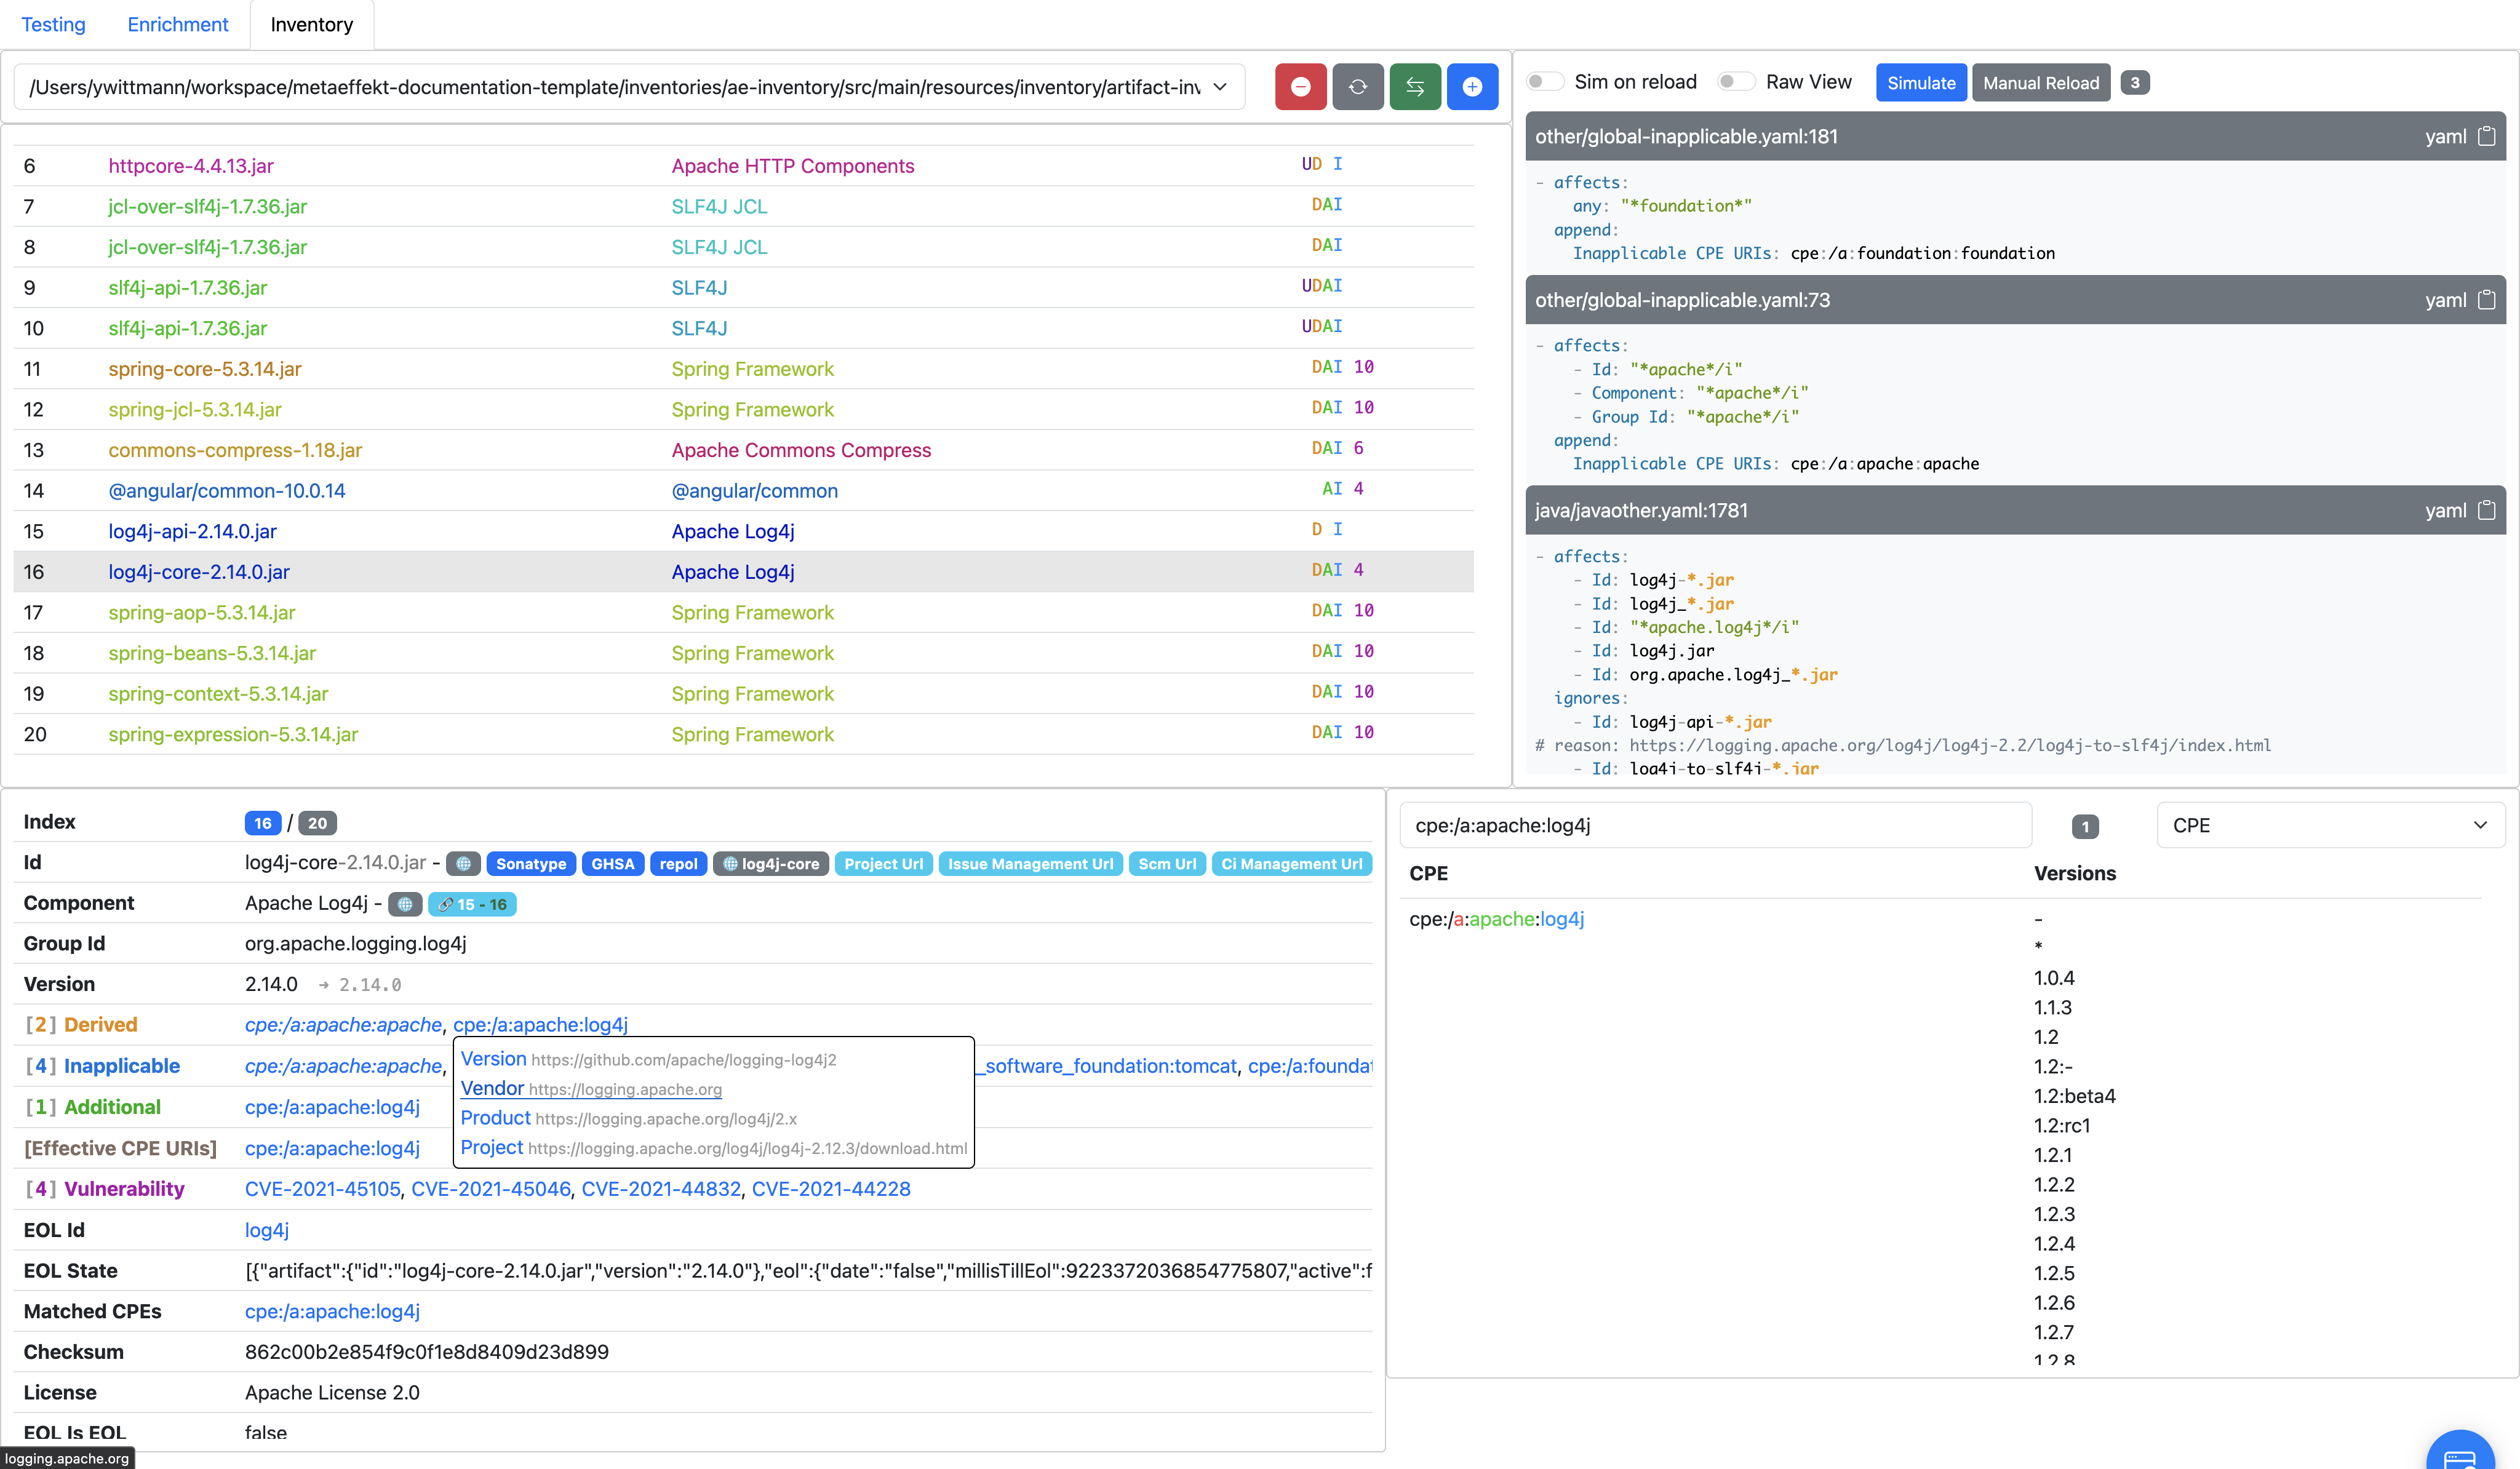
\includegraphics[keepaspectratio,width=1.3\linewidth]{../../images/correlation-utilities-demo}}
    \caption{Das Artefakt \texttt{log4j-core-2.14.0.jar} in den Correlation Utilities}
    \label{fig:correlation-utilities-demo}
\end{figure}

Ein weiteres Widget auf der rechten Seite zeigt, welche Korrelationseinträge auf das aktuelle Artefakt angewendet wurden und erlaubt über eine Integration mit IntelliJ IDEA den direkten Zugriff auf die Korrelationseinträge im Editor und schlägt auf der Basis von einigen bekannten Mustern neue Einträge vor, die mit einem Klick übernommen werden können.
Die Korrelationseinträge werden automatisch bei Änderungen in den Dateien neu geladen und ausgewertet.
Unten rechts kann eine integrierte Abfrageschnittstelle zu den lokalen Datenbanken gefunden werden, über die Abfragen etwa zu \acrshortpl{cpe}, \acrshortpl{cve} oder Produktversionen getätigt werden können.

% TODO: actually perform test, ask Julian
% \smallskip
% Nach einem internen Test hat sich herausgestellt, dass Mitarbeiter mit den Utilities mehr als 2.5-mal so schnell dieselbe Arbeit in höherer Ergebnisqualität durchführen konnten, wie wenn sie dieses Tool nicht verwendet hätten.

\paragraph{Fallunterscheidungen je Artefakt}
Für den allgemeinen Arbeitsablauf mit diesem Tool gibt es pro Artefakt mehrere Fälle, die auftreten können:

\begin{itemize}
    \item Wenn das Artefakt \enquote{Derived CPE URIs} hat, die nicht von einem der weiteren \acrshort{cpe}-Attribute (Additional, Ignores, \ldots) abgedeckt sind, dann bedeutet dies, dass die \acrshortpl{cpe} noch nicht manuell behandelt und geprüft wurden.
    Diese Art von \acrshort{cpe} auf einem Artefakt nennt sich im Tool \enquote{Untouched CPEs}.
    Nachdem sie auf ihre Richtigkeit geprüft wurden, muss die Entscheidung über einen vorhandenen oder neuen Korrelationseintrag in einem der manuellen \acrshort{cpe}-Attribute festgehalten werden.
    Doch nicht nur die automatisch hinzugefügten \acrshort{cpe} müssen untersucht werden, es muss auch nach zusätzlichen \acrshortpl{cpe} im Internet oder den lokalen Datenbanken gesucht werden, um sicherzustellen, dass alle korrekten \acrshort{cpe} gefunden werden.

    \item Wenn das Artefakt nur manuelle \acrshort{cpe}-Attribute gesetzt hat, dann handelt es sich bei diesem Artefakt um ein bereits bekanntes, welches in der Vergangenheit einmal bearbeitet wurde.
    In den meisten Fällen ist hier keine neue Arbeit nötig.
    Manchmal jedoch gibt es Fälle, in denen ein Artefakt seit der letzten Analyse eine neue \acrshort{cpe} zugewiesen bekommen hat, etwas bei dem vorherigen Durchgang übersehen wurde, oder es sich um eine Fehlidentifikation in den Korrelationsdaten handelt und diese fehlerhaft hinzugefügt wurde.
    Je nach Attribut-Kombination sind unterschiedliche Fälle wahrscheinlicher, für welche eine Person mit der Zeit ein Gefühl bekommt.

    \item Wenn das Artefakt überhaupt keine \acrshort{cpe}-Information hat, dann muss manuell nachgeprüft werden, ob es zusätzliche gibt, die diesem Produkt entsprechen.
    Wenn eine oder mehrere passende gefunden werden, wird mit diesen ein neuer Korrelationseintrag angelegt.
\end{itemize}

Vor allem bei einem ersten Durchlauf eines Software-Inventars treten die ersten beiden Fälle häufig auf, aber auch bei erneuten Analysen bekannter Inventare müssen die Artefakte auf ihre Richtigkeit geprüft werden.


\section{Schwächen und Herausforderungen des aktuellen Korrelationsformats}\label{sec:current-correlation-weaknesses}

% https://metaeffekt.atlassian.net/wiki/spaces/KM/pages/3037888514/TBD+New+Correlation+System

Das aktuelle Korrelationsformat hat die letzten Jahre genügend gut funktioniert, um weiterhin verwendbar zu bleiben.
Trotz der hohen Anzahl von über 6400 Korrelationseinträgen von denen die meisten reguläre Ausdrücke auf mehreren Artefaktfeldern prüfen können auch große Software-Inventare in wenigen Sekunden durch alle Einträge geprüft werden (300 Artefakte durchgearbeitet in 3 Sekunden, inklusive Auslesen der Dateien aus dem Dateisystem und Parsen der Einträge).

\subsection{C-01: Übergeneralisierung in Artefakt-Selektoren}\label{subsec:c-01-unspezifische-identifikation-von-artefakten}

% Currently, there are many entries (almost all) that rely on the * wildcard in the Id field to match components version-agnostically. This is not a maintainable approach, since shorter or more common identifiers tend to either be overloaded with multiple components sharing a name, or beginning with the other’s full name. For example:
% - affects:
%     - Id: auth-*.jar
%
% would not only affect an artifact auth-1.2.3.jar, but also auth-registration-helpers-1.2.3.jar. To currently mitigate this, an ignores entry has to be added to the original entry for every single one of these cases.
% - affects:
%     - Id: auth-*.jar
%   ignores:
%     - Id: auth-registration-helpers-*.jar
%
% Fields like the Component cannot be used reliably, since they are often hand-filled or not standardized. Fields like the PURL are more common these days, but still not available on every generated inventory. The artifact Type is still not a normalized field, although it hopefully soon will be (

Wie in \autoref{sec:metaeffekt-inventory-format} erwähnt ist die \texttt{Id} eines Artefakts das einzige Attribut, welches zuverlässig unabhängig des Software-Ökosystems immer gesetzt ist.
Daher dient es in den meisten Korrelationseinträgen auch als Hauptmerkmal, anhand von dem ein Artefakt identifiziert wird.
Leider ist die \texttt{Id} nicht besonders Matching-Freundlich, da sie Versionen und Dateiendungen enthält, sodass bei einem Vergleich nicht auf Gleichheit geprüft werden kann.

Die meisten existierenden Einträge verlassen sich daher auf den Platzhalter (\texttt{*}) im Feld \texttt{Id}, um versionierungsunabhängig zu matchen.
Dieser Ansatz ist aber nicht nachhaltig, da kürzere oder häufig vorkommende Bezeichner von Artefakten zu Mehrdeutigkeiten führen:
So würde ein Eintrag für \texttt{auth-*.jar} sowohl \texttt{auth-1.2.3.jar} als auch \texttt{auth-registration-helpers-1.2.3.jar} erfassen, zur Abhilfe müssen manuell \texttt{ignores}-Einträge für jede Ausnahme erstellt werden.
Felder wie \texttt{Component} mit ihren konkreten Komponentenbezeichnern sind bedauerlicherweise ebenfalls unzuverlässig, da sie teils manuell gepflegt und teils automatisch abgeleitet werden und über Inventare nicht immer einheitlich sind.
Obwohl \acrshort{purl}-basierte Identifikation in den \metaeffekt-Inventaren zunimmt, ist sie bei weitem noch nicht flächendeckend genug verfügbar um diese als Hauptkriterium verwenden zu können.

\subsection{C-02: Inkonsistente und fehlende Artefakt-Typisierung}\label{subsec:c-02-uneindeutige-artefakt-typinformation}

% AE-556: [Artifact Analysis] Define [Artifact Type] / [Component Source Type], create Data Types and apply consistently across code baseTo Do).
% It would be nice if there was a smarter preprocessing step, that would attempt to recover this kind of information in a normalized way, based on several different criteria. The ones listed below are merely examples to illustrate what could be done, this is to be defined:
%     Actual component name
%         Check if there is a PURL and whether it matches with either Component or the Id
%         Check whether the Id contains the Component
%         Fallback to Id
%     Actual component type / ecosystem
%         Consists of a component category (web-module) and a subcategory (nodejs-module)
%         This will be available more generally in the future, but for now this information would have to be guessed from the available fields Type, PURL, etc.
%         This information would be very useful to limit the matching of an entry to a single ecosystem, without affecting others.
%     Version
%         The version field is already fairly normalized, but maybe add a nicer way to compare versions with the component version instead of the huge entry that is currently required for this
% These computed values can be used in the component identification as listed below to reduce the ambiguity in matching and reduce the complexity of the data.
%
% Basically: Enable better, ecosystem-specific matching of artifacts.
% Simply to get the idea across, something like this:
% - affects:
%   - matcher type: maven
%     group id: com.x
%     artifact id: some-artifact

In \autoref{subsec:analysis-ae-software-inventories} wurden die drei Inventar-Attribute \texttt{Type}, \texttt{Specific Type} und \texttt{Ecosystem} identifiziert, auf denen der Typ eines Artefakts \textit{meist} basiert.
Jedoch haben diese mehrere Probleme:

\begin{itemize}
    \item Typbezeichnungen sind auch innerhalb Ökosystemen in manchen Fällen inkonsistent zu sich selbst, indem die Attribute für dasselbe Ökosystem unterschiedliche Wertekombinationen verwenden.
    So sind etwa \texttt{web-module → npm-module}, \texttt{nodejs-module → npm-module} und \texttt{npm-module → <empty>} alle gültige Darstellungsformen für den Typ eines NPM-Moduls.
    Dies verhindert eine normalisierte Klassifikation und erklärt die Notwendigkeit für Ausdrücke wie \texttt{Type: /(web|nodejs|npm)-module/} in der Abfragelogik in den Korrelationseinträgen um alle Ausprägungen mit einem Eintrag abdecken zu können.

    \item Je nach Erzeugungsquelle und den konkreten Ursprüngen der Inventare haben Artefakte nicht immer Typ-Informationen angeheftet.
    So kann man sich nicht immer darauf verlassen, dass ein Typ vorhanden ist und muss auf andere, implizitere Eigenschaften wie Dateiendungen (\texttt{.jar} bei Java-Artefakten) prüfen.

    \item Viele Software-Ökosysteme und Typen haben in den \metaeffekt-Systemen keinen offiziellen Typ, auf den geprüft werden kann oder der gesetzt sein könnte.
    Hierzu zählen etwa Ruby Gems \footnote{\url{https://rubygems.org}} oder Rust mit Crate\footnote{\url{https://crates.io}}, aber auch viele weitere die nicht eindeutig identifiziert werden können.
\end{itemize}

Eine Normalisierung dieser Felder ist seit einiger Zeit geplant, jedoch ist hierzu noch keine Arbeit geschehen.

\subsection{C-03: Duplizierte Artefakt-Selektoren}\label{subsec:c-03-duplizierte-artefakt-selektoren}

% doppelt weil aufeinander aufbauende einträge
% wenn ein feld unterschiedlich gleich neuer eintrag
%   vererbung als lösung

Häufig müssen ähnliche Artefakt-Selektoren für unterschiedliche Korrelationseinträge dupliziert werden.
Aktuell existiert kein Mechanismus zur Vererbung oder Wiederverwendung von Attributen zwischen Korrelationseinträgen.
Wenn sich also eine Produktidentifikation in nur einem Attribut unterscheidet, müssen zwei getrennte Einträge mit fast komplett identischen Attributmengen erstellt werden.
Die einzelnen Attribute, die als Determinate für die übrigen Attributwerte dienen, können leicht variieren und führen so zu redundanten Einträgen mit hohem Wartungsaufwand.

Wie im Beispiel in \autoref{lst:duplicate-artifact-selectors} zu sehen ist, unterscheidet sich die Attributmenge nur in einem Attribut, der \texttt{Architecture}.
Dennoch müssen alleine für diese zwei \enquote{MS Product IDs} zwei nahezu identische Korrelationseinträge gepflegt werden, und in der Realität gibt es wesentlich mehr, die hier angegeben werden müssen.

\begin{lstlisting}[style=yaml,caption={Zwei Korrelationseinträge mit nahezu identischen Attributen},label={lst:duplicate-artifact-selectors}]
- affects:
    - Id: Microsoft Windows 10
      Version: 10.0.19044
      Type: operating system
      Architecture: "64"
    - Id: Windows 10  # no "Microsoft"
      Version: 10.0.19044
      Type: operating system
      Architecture: "64"
  append:
    MS Product ID: "11931"

- affects:
    - Id: Microsoft Windows 10
      Version: 10.0.19044
      Type: operating system
      Architecture: "32"
  append:
    MS Product ID: "11929"
\end{lstlisting}

Dieses Beispiel offenbart ein weiteres Problem der Artefakt-Matcher:
Pro Attribut ist nur ein Wertvergleich möglich.
Sobald es also zwei oder mehr Varianten für ein Feld existieren, müssen entweder reguläre Ausdrücke verwendet, oder der gesamte Eintrag dupliziert werden.

\subsection{C-04: Große Korrelationsdateien als Wartungsproblem}\label{subsec:c-04-groe-und-unubersichtliche-yaml-dateien}

% Find a way to better split the entries into multiple files. The 6000-lines files are not only tedious to work with, but also require unnecessarily large amounts of computational power to render, with a notable slowdown of the IDE in use.
% Maybe, as suggested below, YAML files could not even be required for this, maybe another data format would be better suited. We will see.

Der aktuelle Korrelationsdatensatz der \metaeffektsp umfasst fast 30000 Zeilen an \acrshort{yaml}, die manuell erstellt wurden.
Die Performanz ist wie bereits festgestellt kein Problem, eher die Übersichtlichkeit über diese großen Datenmengen.

\subsection{C-05: Unstrukturierte und unklare Entscheidungsbegründungen}\label{subsec:c-05-reason-not-good-enough}

% The current “reason” format is a simple, unstructured text comment. It is not machine-readable or evaluate-able in any way.
% The current format has a loosely defined arrow reasoning chain syntax that looks like this (fake values) cpe:/a:apache:commons_io --> https://github.com/apache/commons-io --> "library for doing IO operations" --> same library as artifact
% Since the content is only a simple text comment in a YAML file, it is impossible for the parser to extract this information and use it somehow to generate more descriptive views on the reason a connection between components and product identifiers has been made.
% This new format should therefore be in a machine-readable format inside the data structure of the connections. This makes it harder for a human correlation assistant to create the data, therefore the user should not have to edit this reason manually, but rather via a UI that they can click “apply” on or similar.

Wann auch immer ein neuer Eintrag erstellt, eine neue Identifikation hinzugefügt, oder allgemein eine Entscheidung gefällt wird, sollen die entsprechenden Teammitglieder eine textuelle Begründung verfassen, anhand der sich diese später nachvollziehen lassen kann.
Es wurde zudem ein Konsens geschlossen, dass eine schrittbasierte-Syntax verwendet wird, die jeden Schritt in der Herleitungskette einer Information mit einem \enquote{\texttt{-->}} trennt.
Die aktuelle \enquote{reason}-Dokumentation besteht allerdings nur aus einem unstrukturierten Textkommentar über dem Korrelationseintrag im \acrshort{yaml}.
Diese sind nicht maschinenlesbar, oft unvollständig oder vage und werden manchmal aus diversen Gründen nicht angelegt, was die spätere Nachvollziehbarkeit nicht fördert.

Beispielketten können sein:

\begin{itemize}
    \itemsep0em
    \item \texttt{cpe:/a:apache:commons\_io --> https://github.com/apache/commons-io --> "library for IO operations" --> same as artifact}
    \item \texttt{cpe:/a:golang:crypto --> https://github.com/golang/crypto / https://golang.org/x/crypto --> by golang (Go, [mirror] Go supplementary cryptography libraries) --> version range matches artifact}
    \item \texttt{cpe:/a:setorinformatica:sil --> CVE-2024-22633 --> https://tomiodarim.io/posts/cve-2024-22632-3 --> "Setor Informatica is a Brazilian company that develops software for the Brazilian market" / "Smart System for Laboratories (S.I.L.)" --> they reported a vulnerability for another S.I.L. software --> cpe is applicable}
\end{itemize}

\subsection{C-06: Keine Einträge für Negatividentifikationen}\label{subsec:c-06-falle-ohne-aktion-konnen-nicht-dokumentiert-werden}

% If an artifact lacks any CPE or other identifiers, a correlation assistant may have already put in significant effort to reach this point. He might have had to make quite the research or other logical conclusions.
% But, in the current system, such cases \textit{cannot} at all be put into the correlation files. A separate (non-normalized or used) file would have to be used to keep this knowledge. But such an additional system does not exist yet, so nothing is done to document the effort and the information is lost.
% The next time a person sees this artifact and either does not remember the effort from last time, or is a completely new person with a fresh perspective, they cannot build on the research that was already made.

Wenn eine Person ein Artefakt ohne \acrshort{cpe} darauf analysiert, ob diese Abwesenheit korrekt ist, oder ob noch Angaben fehlen und es sich herausstellt, dass das Artefakt tatsächlich keiner \acrshort{cpe} zuordenbar ist, kann der Forschungsaufwand hierfür im aktuellen System nicht dokumentiert werden.
Das liegt daran, dass ein Korrelationseintrag nur dann gültig ist, wenn er eine Selektion und eine Modifikations-Aktion definiert, und damit gibt es keinen Eintrag, auf den die Erkenntnisse notiert werden könnten.
Diese Wissenslücke führt zu wiederholtem Aufwand bei erneuten Analysen desselben Artefakts, da das Wissen über die korrekte Abwesenheit verloren gegangen ist.

\subsection{C-07: Schlechtes Testframework, wenig Unterstützung für automatisierte Kontrolle}\label{subsec:c-07-test-framework}

% The current correlation system does have a “validation” format that allows for the manual creation of test cases for the created correlation entries, but it’s quite tedious to use.
% It would be much nicer, if the system used to create the correlation data (e.g. correlation utilities) would automatically (or with the press of a button) record the artifact the correlation was created on, the before and after states and create a test case with an expected result based on that.
% Through the more documentation-heavy new format, these tests may also already be self-documenting.

Existierende Testfälle für Korrelationseinträge werden manuell in einem separaten Validierungsformat gepflegt, was in seiner Konfiguration aufwendig ist.
Dieser Aufwand führt dazu, dass es in der Realität nicht von den Mitarbeitern verwendet wird, und so nur ein sehr kleiner Datensatz an automatisierbaren Testfällen existiert.

\subsection{C-08: Generierte YAML-Dateien}\label{subsec:c-08-generated-correlation-data}

% The generated directory contains several automatically generated YAML correlation files, based on the data that is present in the index when generating.
% These need to be converted into the new format somehow.

Die automatisch generierten \acrshort{yaml}-Dateien, wie in \autoref{subsec:old-generated-correlation-data} gezeigt, müssen bei Datenänderungen manuell neu generiert werden, was nicht intransparent ist.
Zudem haben sich, vor allem bei den JRE/JDK-Generatoren einige Probleme mit der Abbildung auf das aktuelle Korrelationssystem gezeigt, die nur über die Verwendung von inkrementellen Korrelationseinträgen und dem Attribut \texttt{CPE URIs} (welches nicht mehr verwendet werden soll) gelöst werden konnten.
Da eine der Anforderungen an das neue Korrelationssystem ist, weitere dynamische Quellen zu integrieren, muss dieses Konzept für generierte Daten von Anfang an mitgedacht werden.

\subsection{C-09: Teilen öffentlicher Anteile}\label{subsec:c-09-sharing-of-public-data}

% darüber reden, dass der terms metadata-datensatz ja auch mit dem Kosmos https://github.com/org-metaeffekt/metaeffekt-kosmos die öffentlichen aspekte freigibt
% man könnte das hier ja genau so machen, aber im moment ist alles ein gemischter datensatz
% im neuen inkrementellen konzept soll das am besten über mehrere datenquellen auftrennbar sein
% daten die aus öffentlichen datenquellen abgeleitet wurden

Der aktuelle Korrelationsdatensatz besteht im Moment zu einem Teil aus den generierten Korrelationseinträgen aus öffentlichen Datenquellen, und zum anderen aus unternehmensintern für spezifische Kunden recherchierten Daten.
Da diese Daten direkt nebeneinander in den gleichen Verzeichnissen liegen, erschwert dies die Auftrennung.
Da in dem manuellen Teil dieses Datensatzes viel Firmenzeit geflossen ist, stellt dieser einen der lizenzierbaren Bausteine der \metaeffektsp dar und ist damit nur kostenpflichtig erwerblich.

Analog zum bereits existierenden \enquote{\metaeffekt-kosmos}-Projekt\footnote{\url{https://github.com/org-metaeffekt/metaeffekt-kosmos}}, welches den Open-Source-Anteil der \metaeffekt-Lizenzdatenbank öffentlich frei verfügbar zugänglich macht, könnte ein Konzept eingeführt werden, bei dem die automatisch generierten Einträge ohne die manuellen Arbeiten auf eine ähnliche Weise verfügbar gemacht werden, damit jeder eine gewisse Grundqualität der Ergebnisse erhält.
So können firmeninterne Ergänzungen weiterhin in einem separaten, nicht öffentlichen Datensatz verteilt werden.

\subsection{C-10: Reihenfolgenbedingte Seiteneffekte von Einträgen}\label{subsec:c-10-order-dependency}

% Die inkrementelle Anwendung von Korrelationseinträgen erfordert eine strenge Reihenfolge, die aktuell nur durch die Position in der \acrshort{yaml}-Datei gesteuert wird. Änderungen in der Eintragsreihenfolge können unbeabsichtigte Seiteneffekte verursachen. Explizite Abhängigkeitsdeklarationen oder eine deklarative Priorisierungslogik (anstatt impliziter Dateiordnung) würden Robustheit und Verständlichkeit erhöhen.

Das aktuelle System für Korrelationseinträge verarbeitet die Daten inkrementell (siehe \autoref{par:incremental-correlation-entries}), d.h.\ jeder Eintrag baut potenziell auf dem Zustand auf, der durch vorherige Einträge erarbeitet wurde.
Da diese Abhängigkeiten zwischen Einträgen nicht explizit deklariert werden müssen, ergibt sich die Reihenfolge innerhalb einer \acrshort{yaml}-Datei wenigstens noch basierend auf der Position innerhalb der Datei, Dateiübergreifend jedoch ist die Verarbeitungsreihenfolge arbiträr basierend auf der Ordnung, die das Dateisystem dem Programm übergibt.
Dies macht das System empfindlich gegenüber Umordnungen der Einträge, vor allem wenn über Dateien hinweg absichtlich oder unabsichtlich Abhängigkeiten erstellt wurden.

Ein Beispiel für eine solche Situation ist in \autoref{lst:correlation-order-depdendency-example} dargestellt, deren beide Korrelationseinträge in zwei separaten Dateien aufgeführt sind.
Der erste Eintrag ergänzt eine Liste an \acrshortpl{cpe} ganz allgemein für \texttt{redis}-Artefakte in dem \texttt{Additional CPE URIs}-Attribut.
Der zweite hat nun das Ziel, diese für das Python-Modul \enquote{redis}\footnote{\url{https://pypi.org/project/redis}} als nicht zutreffend zu markieren.
Dafür müssen die \acrshort{cpe} über das \texttt{remove}-Schlüsselwort zunächst wieder aus dem \texttt{Additional CPE URIs}-Attribut entfernt, und dann explizit als \texttt{Inapplicable CPE URIs} für das Python-Modul gesetzt werden.
Wenn nun die Verarbeitungsreihenfolge der Einträge sich durch eine Verschiebung oder Umbenennung der Dateien ändert, dann wird auch diese Logik nicht mehr korrekt greifen können.

\begin{lstlisting}[style=yaml,caption={Korrelationseinträge in zwei unterschiedlichen Dateien, die aufeinander aufbauen},label={lst:correlation-order-depdendency-example}]
- affects:
    - Id: redis-*/i
      Component: redis/i
  append:
    Additional CPE URIs: cpe:/a:redis:redis, cpe:/a:redislabs:redis, cpe:/a:pivotal_software:redis
    EOL Id: redis
- affects:
    - Id: redis-*/i
      Type: python-module
  remove:
    Additional CPE URIs: cpe:/a:redis:redis, cpe:/a:redislabs:redis, cpe:/a:pivotal_software:redis
  append:
    Inapplicable CPE URIs: cpe:/a:redis:redis, cpe:/a:redislabs:redis, cpe:/a:pivotal_software:redis
    Additional CPE URIs: cpe:/a:redis:redis-py
\end{lstlisting}

\subsection{C-11: YAML-Eintrag finden}\label{subsec:c-11-finding-yaml-entries}

Die Correlation Utilities, wie in \autoref{subsec:correlation-utilities} vorgestellt, erlauben es mit einem Klick auf einen Korrelationseintrag zu diesem in der entsprechenden \acrshort{yaml}-Datei zu springen.
Das Problem hierbei liegt darin, dass das aus dem \acrshort{yaml} erzeugten Datenmodell von sich aus keine Referenz mehr auf die Zeilennummern der Datei enthält.
Weiterhin werden einige Transformationen an den Attributen vorgenommen, wie etwa das Parsen der unterschiedlichen Darstellungsweisen für reguläre Ausdrücke, sodass nicht mehr einfach so die Originalinhalte mit dem Datenmodell abgeglichen werden können.
Es wird daher im Quelltext der \acrshort{yaml}-Dateien Zeile für Zeile jeder Eintrag nach gewissen Schlüsselwörtern aus dem Datenmodell abgesucht, und der mit der höchsten Übereinstimmungsrate wird ausgewählt.

Dieser Prozess funktioniert bei einer großen Anzahl der Einträge, jedoch kann es bei sehr ähnlichen Einträgen oder jenen, die viele komplizierte reguläre Ausdrücke verwenden passieren, dass die Zuordnung nicht erfolgreich ausgewertet wird.


\section{Anforderungen an das neue Korrelationssystem}\label{sec:requirements}

% “4.3. Data Types in Falcon” ([Cheramangalath et al., 2016, p. 6](zotero://select/library/items/4DG8G9J3)) ([pdf](zotero://open-pdf/library/items/QNYKYEH4?page=6&annotation=C7MKFAUG))

Basierend auf der Analyse der bestehenden Herausforderungen und weiteren Rahmenbedingungen werden die Anforderungen an das neue Korrelationssystem abgeleitet.

\subsection{A-01: Graphenbasiertes Datenmodell mit expliziten Abhängigkeitsdeklarationen}\label{subsec:req-format-product-graph}

Das Kernmodell des neuen Systems muss als gerichteter Graph implementiert werden, wobei Knoten typisierten Produktrepräsentationen (Artefakte, \acrshort{cpe}, \acrshort{eol}-Id, MS Product ID) repräsentieren und Kanten Relationen mit unterschiedlichen Typen zwischen diesen darstellen.
Kantentypen umfassen mindestens \enquote{is} (represented by, positive Zugehörigkeit) und \enquote{is not} (not represented by, expliziter Ausschluss).
Der Typ des Zielknotens einer Relation entscheidet, wie die Art der Relation interpretiert werden soll.

Jede Repräsentation eines Produkts darf sich in nur einen Knoten ausprägen, Mehrfachreferenzen auf dieselbe Repräsentation müssen durch Kanten auf einen einheitlichen Knoten dargestellt werden.
Dies löst die Reihenfolgenabhängigkeit (\hyperref[subsec:c-10-order-dependency]{C-10}), indem die Abhängigkeiten zwischen Knoten explizit deklariert werden.
Diese Deklaration soll eine topologische Sortierung während der Verarbeitung erzwingen und implizite Dateireihenfolgeabhängigkeiten vollständig entfernen.

Um die programmatische Erfassung eines Knotenpunktes zu ermöglichen, soll jeder Knotenpunkt einen textuellen Identifikator besitzen, der in Kombination mit dem Knotentyp im Graph eindeutig ist.
So kann über die Typ-Id-Kombination jeder Knoten im Graph angesprochen werden.

Der Graph ist gerichtet, damit über die Kantenrichtung die \enquote{is}- und \enquote{is not}-Beziehungen klar ausgewertet werden können.
Falls es nötig ist, kann eine identische, umgekehrte Kante dazu verwendet werden, um die Richtung der Kante auf beide Seiten zu erweitern.
In den Fall, dass der Bedarf besteht herauszufinden, welche weiteren Repräsentationen eine Produktrepräsentation noch haben kann, muss damit also bei dem als \enquote{sich selbst} identifizierten Knoten eine Durchquerung des Graphen unter Berücksichtigung der Kantenrichtung- und Typen gestartet werden, bis alle erreichbaren Knoten gefunden und ausgewertet wurden.

Mit diesem System sollen jedwede Produkte und Repräsentationen modelliert werden können.
Dies löst die Herausforderung \hyperref[subsec:c-06-falle-ohne-aktion-konnen-nicht-dokumentiert-werden]{C-06}, dass keine Identifikationen ohne bekannte Relationen modelliert werden können, da in diesem System dennoch ein Knotenpunkt für die Identifikation erstellt werden kann, ohne eine Relation zu einem weiteren Knoten erstellen zu müssen.

\subsection{A-02: Produkt-Konzept}\label{subsec:req-product-concept}

Wichtig ist die Unterscheidung zwischen einem \textit{Produkt}, und der \textit{Repräsentation eines Produkts} (she.\ \autoref{subsec:produkte-vs-reprasentation}).
Diese sollen sich zwar im Graphen beide als Knotenpunkte darstellen, jedoch muss zwischen ihren Typen unterschieden werden.

So könnte eine Repräsentation mit einer Kante auf einen Produkt-Knotenpunkt verweisen und von diesem eine Kante auf eine weitere Repräsentation des Produkts um anzugeben, dass diese Repräsentationen das selbe Produkt darstellen.

Produktknoten sollen in der Lage sein, Metainformationen über die zugehörigen Repräsentationen abzulegen.
Dazu gehören vor allem Informationen über die Versionsräume und wie zwischen diesen umgewandelt werden kann.

\subsection{A-03: Normalisierte Typidentifikation und typspezifische Attribute für Software-Artefakte}\label{subsec:req-type-specific-matching}

Um die Herausforderung \hyperref[subsec:c-02-uneindeutige-artefakt-typinformation]{C-02} der multiplen Ausprägungen und inkonsistenten Typinformationen zu lösen muss eine Typinferenz-Logik den Artefakttypen konsistent aus multiplen Quellen aufbereiten.
In \autoref{subsec:analysis-ae-software-inventories} wurden die häufigsten Muster für Typinformationen analysiert.
Die Ausgabe der Typinterferenz soll diese verwenden, um normalisierte Ökosystembezeichner (z.B. \texttt{java-module}, \texttt{npm-package}, \texttt{python-module}), als Artefaktattribut verfügbar machen.

Basierend auf dem erkannten Ökosystem/Typ eines Artefakts werden dann weitere Extraktoren auf die Artefakt-Metadaten angewendet.
Diese müssen weitere Attribute als First-Class Matching-Kriterien auf den Artefakt-Selektoren zur Verfügung stellen, wie etwa Maven-Koordinaten (Group Id, Artifact Id) für Java, Paketnamen für NPM, Distributionskennung für Linux-Pakete, Java Runtime-Provider, \ldots.
Wildcard-Selektor wie bisher häufig in der \texttt{Id} (\hyperref[subsec:c-01-unspezifische-identifikation-von-artefakten]{C-01}) können so durch exakte, ökosystemspezifische Attributvergleiche ersetzt werden.

\subsection{A-04: Vererbung von Artefaktmerkmalen}\label{subsec:req-selektor-inheritance}

Um zu vermeiden, dass Artefakt-Selektoren wie in \hyperref[subsec:c-03-duplizierte-artefakt-selektoren]{C-03} für ähnliche Identifikationen wiederholt werden müssen, soll es ein Vererbungssystem an Artefakt-Selektoren geben.
Ein Basis-Selektor definiert generische Selektorattribute (z.B.\ für alle Microsoft Windows-Varianten), während abgeleitete Selektoren spezifische Erweiterungen (z.B.\ Architektur) hinzufügen, wobei lokale Attributdefinitionen geerbte überschreiben.
Dies erlaubt das Teilen von Basisattributen zwischen mehreren spezifischeren Ausprägungen eines Artefakts, ohne die Basisattribute bei jeder Ausprägung wiederholen zu müssen und vermeidet damit zu pflegende Redundanz.
So muss ebenfalls nur der Basis-Selektor angepasst werden, wenn neue Attribute dazukommen oder vorhandene bearbeitet werden sollen.

\subsection{A-05: Auflistung mehrerer Werte pro Attribut}\label{subsec:req-multiple-attribute-values}

In \hyperref[subsec:c-03-duplizierte-artefakt-selektoren]{C-03} wurde die Herausforderungen der mehreren Werte pro Attribut aufgeführt.
Um dieses zu lösen, soll im neuen Modell ein Abgleich von mehreren Optionen möglich sein, bei der nur ein Attributwert übereinstimmen muss (oder-Verknüpfung).

\subsection{A-06: Unterstützung regulärer Ausdrücke}\label{subsec:req-regex-support}

Auch wenn im neuen Format über \hyperref[subsec:req-type-specific-matching]{A-03} die Anzahl der Wildcard-Selektor drastisch verringert werden, soll dennoch das in \autoref{sec:current-correlation-format} beschriebene inkrementelle Wildcard-System weiterhin bestehen bleiben.

\subsection{A-07: Manuelle Modifikation des Graphen}\label{subsec:req-manual-format-modification}

Da in dem neuen Korrelationssystem noch immer manuelle Korrekturen an der automatischen Erkennung von \acrshort{cpe} gemacht werden können sollen, muss ein neues \acrshort{yaml}-basiertes Format entwickelt werden, welches einen solchen Produkt-Graphen modifizieren kann.
Die durchführbaren Modifikationen am Graphen müssen mindestens die Erstellung, Modifikation und Entfernung von Knotenpunkten jedes Types, und die Erstellung, Modifikation und Entfernung von Kanten zwischen Knoten beinhalten.
Technisch sollte dieses Modifikationsformat auf eine Weise modelliert werden, dass jegliche nötigen Modifikationen am Graphen ausschließlich darüber lösbar sind, ohne weiteren Code schreiben zu müssen, um als allgemeine Schnittstelle für Graphmodifikationen zu dienen.
Auf diese Weise können auch andere Prozesse die selbe Logik verwenden, um ihre Änderungen durchzuführen, mit den gleichen Garantien wie der manuelle Prozess.

Da die Kombination aus Typ und Id jedes Knotens im Graphen eindeutig ist (she. \hyperref[subsec:req-format-product-graph]{A-01}), sollte auch das Modifikationsformat diese Weise verwenden, Knotenpunkte für die Modifikation zu selektieren.

Das neue Korrelationssystem als Graph zu modellieren führt viele Komplexitäten ein, die für den Nutzer im manuellen Modifikationsformat abstrahiert werden müssen, um noch immer so effektiv wie im alten Format arbeiten zu können.
Hierfür muss ein Format iterativ entworfen und mit aktuellen Nutzern des Formats getestet und abgesprochen werden, um es so einfach wie möglich zu machen, den Graphen zu modifizieren ohne Kontrolle über detaillierte Attribute zu verlieren.

Da das alte Format oft Schwierigkeiten hatte, aus dem Datenmodell wieder die ursprünglichen Einträge in den \acrshort{yaml}-Dateien zu finden (she.\ \hyperref[subsec:c-11-finding-yaml-entries]{C-11}), soll in dem neuen \acrshort{yaml}-Modifikationsformat das Auffinden von Einträgen deterministisch gestaltet werden.
Wenn zur Selektion der Knotenpunkte im \acrshort{yaml} der Typ und die Id verwendet wird, dann kann diese auch umgekehrt wieder aus dem Graphen ausgelesen und die zugehörige Zeile im \acrshort{yaml} gefunden werden.

\subsection{A-08: Maschinenlesbare Entscheidungsdokumentation}\label{subsec:req-reason-format}

Um Daten wie Projektreferenzen, Beschreibungen und Begründung für Entscheidungen im Gegensatz zum alten Korrelationssystem (\hyperref[subsec:c-05-reason-not-good-enough]{C-05}) maschinenlesbar zu machen, müssen die bisherigen Kommentarfelder als strukturierte Objekte mit standardisierten Feldern modelliert werden.
Dies soll es in automatisierten Systemen oder Nutzeroberflächen möglich machen, Metadaten über die Produktidentifikationen nützlicher anzuzeigen und auswerten zu können.

Da das neue Korrelationssystem mit einem Graphen modelliert wird, gibt es zwei Stellen, an denen diese Dokumentation angebracht werden kann und muss.
So wird der frühere \texttt{\# reason:}-Kommentar mit der Begründung der gegenseitigen Anwendbarkeit von Produkten nun auf den Kanten modelliert, und die weiteren Metadaten eines Produkts wie die Beschreibung oder Web-Referenzen auf den Knotenpuntken.

\subsection{A-09: Generierungsframework für dynamische Daten}\label{subsec:req-generated-data}

Im aktuellen Korrelationssystem liegen die generierten \acrshort{yaml}-Dateien gleichwertig neben den manuell gepflegten Daten (\hyperref[subsec:c-08-generated-correlation-data]{C-08}).
Da ihre Existenz nicht von Beginn an geplant war, wurden das Selektor-System und die weiteren Matching-Regeln nicht für die besonderen Anforderungen die diese Quellen mit sich bringen ausgelegt.
Im neuen System soll der gesamte Graph darauf aufbauen, dass er zunächst mit generierten Daten befüllt wird und basierend darauf die manuellen Modifikationen angewendet werden.

Mit den Datensätzen der \metaeffektsp sollen bereits alle Knotenpunkte für \acrshortpl{cpe}, MS Product Ids und \acrshort{eol}-Ids erzeugt werden, die bekannt sind, manche sollen bereits Kanten zwischen den Knoten erzeugen.
Zudem sollen weitere Datenquellen wie die bereits vorhandenen Generatoren für NPM-Pakete zu \acrshortpl{cpe} und die für die vielen Java Runtimes, aber auch neue wie purl2cpe von scanoss\footnote{\url{https://github.com/scanoss/purl2cpe}} dazu beitragen, den Graphen bereits vorzufüllen und die darauf folgende Arbeit zu erleichtern.

Um den fertigen auslieferbaren Graphen zu erhalten, soll zunächst der generierte Anteil des Graphen erstellt werden und dann auf diesem mit den manuellen Modifikationen aufgebaut werden.
Durch diese Trennung in mehrere \enquote{Contributors} am Graphen kann \hyperref[subsec:c-09-sharing-of-public-data]{C-09} einfach abgebildet werden, indem der Datensatz vor der Anwendung des manuellen Schritts ausgeliefert wird.

\subsection{A-10: Qualitätsmetriken des Graphen}\label{subsec:req-graph-inner-consistency}

%- Innere Konsistenz: Zu jeder Repräsentation, die durch das Modell identifiziert werden soll, darf maximal eine
%  eindeutige Identifikation stattfinden und es darf keine losen Knoten geben
%- Datensatz erklärt sich selbst: Zu jedem Eintrag und jeder Verbindung muss es eine Begründung jeglicher Art geben
%- Ein sich selbst prüfender Datensatz: Nachdem ein Datensatz manuell geprüft wurde, werden alle Identifikationen in
%  einem separaten Datensatz abgelegt, um bei zukünftigen Änderungen automatisch geprüft werden zu können. So soll
%  gegeben sein, dass die Identifikation eines bekannten Produktes nicht einfach so ändern kann, ohne, dass man es
%  mitbekommen würde.

Um verifizieren zu können, dass der Graph sinnhaft strukturiert und in sich selbst konsistent ist, müssen einige Prüfungen darauf ablaufen können.
Diese prüfen mindestens die folgenden Eigenschaften:

\begin{itemize}
    \item Zu jeder Repräsentation eines Produkts in dem Graphen darf maximal genau eine eindeutige Identifikation stattfinden.
    Dies bedeutet, dass jeder Knoten exakt eine Repräsentation vollständig modellieren sollte und diese nicht noch einmal von einem anderen Knoten partiell abgedeckt sein darf.
    Diese Metrik muss sowohl in dem Matching-Algorithmus, als auch als Modellierungsvorschrift umgesetzt werden.
    % FIXME-YWI: das hier hat halt das Problem, dass wir den Graphen mit allen CPE, etc. füllen wollen und nicht immer ein zugehöriges Produkt erzeugt werden kann.
    \item Es darf keine losen Knoten geben, jede Repräsentation muss mindestens zu einem Produkt-Knotenpunkt verbunden sein um sicherzustellen, dass mit einer Identifikation auch ein Informationsgewinn stattfinden kann.
    \item Um einen sich selbst erklärenden Datensatz zu erhalten, müssen die Metadaten jedes Knotenpunktes aufgefüllt sein und die Kanten eine Begründung enthalten, warum sie so existieren.
    \item Der Graph soll sich selbst prüfen können: Nachdem ein Software-Inventar manuell geprüft wurde, sollen alle Quell-Artefakte mit ihren Identifikationen in einem separaten Datensatz abgelegt werden, um diese bei zukünftigen Änderungen am Graphen automatisch prüfen zu können.
    So kann die Identifikation eines bekannten Produktes sich nicht einfach so ändern, ohne, dass man es mitbekommen würde.
    \item Eine Prüfung auf zirkuläre Vererbungs-Referenzen soll sicherstellen, dass es immer einen spezifischeren Knoten gibt und keine Schleife entsteht.
\end{itemize}

\subsection{A-11: Organisation der \acrshort{yaml}-Dateien}\label{subsec:req-yaml-file-organization}

Die manuell gepflegten Korrelationsdateien werden noch immer im Dateisystem abgelegt werden.
Hierbei müssen jedoch die Herausforderungen der tausenden Zeilen langen \acrshort{yaml}-Dateien adressiert werden (\hyperref[subsec:c-04-groe-und-unubersichtliche-yaml-dateien]{C-04}).
Es soll für die neuen Dateien mindestens eine Auftrennung in Verzeichnissen nach Typ und/oder Ökosystem geben, und weiterführend können die einzelnen Hersteller- oder Produktgruppen jeweils in getrennten Dateien aufgeführt werden.

\subsection{A-12: Überführung von Einträgen aus dem alten Korrelationsdatensatz}\label{subsec:req-current-dataset-conversion}

Um die Transition zum neuen Korrelationssystem so einfach wie möglich zu machen, sollen die beiden Datensätze zunächst parallel weiter geführt und auf Inventare angewendet werden.
In der Transitionsperiode sollen dann die Einträge aus dem alten Format in das neue konvertiert und damit der alte langsam ersetzt werden.

Dazu muss sichergestellt werden, dass der neue Graph mindestens die Fähigkeiten des alten Formats abdeckt und durch seine weiteren Eigenschaften die Identifikation sogar verbessert.

\subsection{A-13: Performance des neuen Korrelationsformats}\label{subsec:req-correlation-format-performance}

Das alte Korrelationssystem wurde bei unterschiedlichen Inventar-Größen mit dem aktuellen Datensatz mit 6400 Einträgen getestet.
Die Zeiten werden in \autoref{tab:old-correlation-performance} angegeben.

Aus diesen Messwerten sind zwei Phasen erkennbar.
Zunächst läuft eine konstante Startzeit (bei dem getesteten Datensatz etwa 0,8-0,9 Sekunden), die unabhängig von der Anzahl der Artefakte im Inventar auftritt, in welcher die Korrelationseinträge aus dem \acrshort{yaml} ausgelesen werden.
Danach steigt die Laufzeit annähernd linear mit der Anzahl der Artefakte an, der Zeitbedarf pro zusätzlichem Artefakt ist also relativ konstant.

\begin{table}[h!]
    \centering
    \label{tab:old-correlation-performance}
    \begin{tabular}{l r r r r}
        \toprule
        \textbf{Artefakte} & \textbf{Ø [s]} & \textbf{Min. [s]} & \textbf{Max. [s]} \\
        \midrule
        0                  & 0,806          & 0,435             & 1,668             \\
        1                  & 0,897          & 0,453             & 1,919             \\
        500                & 2,033          & 1,504             & 3,277             \\
        1000               & 3,256          & 2,531             & 4,612             \\
        2000               & 5,920          & 4,543             & 6,979             \\
        3000               & 8,804          & 7,425             & 11,800            \\
        4000               & 9,433          & 8,780             & 10,338            \\
        5000               & 12,162         & 10,929            & 13,596            \\
        6000               & 13,609         & 12,461            & 15,381            \\
        \bottomrule
    \end{tabular}
    \caption{Gemessene Laufzeiten des alten Korrelationsformats bei unterschiedlichen Artefakt-Anzahlen.}
\end{table}

Da der Korrelationsschritt bisher bei weitem nicht der zeitintensivste Schritt in der Schwachstellenanalyse ist, ist die Optimierung nie eine kritische Anforderung gewesen.
Das neue Korrelationsmodell sollte diese Zeiten jedoch bei vergleichbaren Datenmengen dennoch nicht um einen Faktor von 2 überschreiten.

% \begin{table}[h!]
%     \centering
%     \label{tab:new-correlation-performance}
%     \begin{tabular}{l r r r}
%         \toprule
%         \textbf{Artefakte} & \textbf{Ø [s]} & \textbf{Min. [s]} & \textbf{Max. [s]} \\
%         \midrule
%         0                  & 0,000          & 0,000             & 0,000             \\
%         1                  & 0,034          & 0,001             & 0,134             \\
%         500                & 2,303          & 2,078             & 2,950             \\
%         1000               & 4,249          & 4,022             & 4,790             \\
%         2000               & 8,582          & 8,109             & 9,658             \\
%         3000               & 12,639         & 12,156            & 13,730            \\
%         4000               & 16,702         & 16,113            & 17,446            \\
%         5000               & 20,693         & 20,179            & 21,175            \\
%         6000               & 24,601         & 24,093            & 25,503            \\
%         \bottomrule
%     \end{tabular}
%     \caption{Laufzeiten des neuen Korrelationsformats bei unterschiedlichen Artefakt-Anzahlen.}
% \end{table}

\subsection{A-14: Auslieferung des Datensatzes}\label{subsec:req-correlation-data-delivery}

Der Aufwand, den Korrelationsdatensatz zu verteilen, muss vergleichbar mit dem alten Korrelationssystem sein.
Bisher hat es ausgereicht, einen Ordner an \acrshort{yaml}-Dateien zu verteilen.
Es darf also keine dedizierte Ausführungsumgebung einer Datenbank vorausgesetzt werden, der gesamte Ablauf muss innerhalb des Java-Prozesses stattfinden, in dem auch das alte Format verwendet wird.


\section{Referenzfälle}\label{sec:reference-case-chapter}

Aus einer Auswertung aus dem bereits vorhandenen Korrelationsdatensatz wurden vier grundlegende Fälle identifiziert, die in ihrer Kombination den Großteil der Komplexität in den bisherigen Daten abdecken.
Sie wurden nicht aufgrund von ihren Inhalten oder betreffenden Produkten gewählt, sondern wegen ihrer Struktur und verwendeten impliziten oder expliziten Mechanismen.
Das neue Modell muss also mindestens diese Fälle abdecken können und daher werden sie als Referenzfälle verwendet.

Neben dem konzeptionellen Unterschied zum neuen Korrelationsformat der Modellierung als Graphen haben diese Beispiele im alten Format zudem die Eigenschaft, dass sie mit dem Ziel erstellt werden, ein Inventar-Artefakt zu modifizieren.
Es wird also immer ausschließlich von einem Artefakt ausgegangen, und dessen Ziel-Attribut-Werte definiert.
Im neuen Format wird dieser Gedanke in den Hintergrund treten, und sich implizit durch den Aufbau des Graphen ergeben.

Es werden zunächst immer die Einträge vorgestellt, dann die Herausforderungen und relevanten Anforderungen identifiziert.
Diese Referenzfälle werden in \autoref{sec:beispiele-fertige-implementierung} jeweils auf das neue Korrelationssystem übersetzt, um einen Vergleich der Formate zu ermöglichen.

% FIXME-KKL: Zusammenhalten: Ich glaube der Kommentar hier bezieht sich darauf, dass im PDF zwischen dem Titel und der Klammer ein Abstand ist. Den habe ich schon versucht wegzubekommen, aber LaTex will das unbedingt so aufteilen.
\paragraph{JavaScript-Paket mit multiplen Namensvarianten}\label{par:reference-case-walletconnect} (s. \autoref{lst:correlation-generated-walletconnect-example})

Bei dem Paket \texttt{@web3-react/walletconnect} handelt sich in der NPM-Registry zwar um ein eindeutiges Paket, allerdings kann sich der Bezeichner in den gescannten Software-Inventaren in unterschiedlichen Varianten ausprägen, auf die alle geprüft werden muss.
In diesem Fall handelt es sich um eine Positividentifikation auf einer \acrshort{cpe} \texttt{cpe:/a:uniswap:web3-react\_walletconnect}, die als \texttt{Additional CPE URIs} zum Artefakt hinzugefügt wird.
Um die drei alternative Namensformen in dem Selektor in der \texttt{affects}-Sektion erfassen zu können, müssen diese alle separat mit Wiederholung der restlichen Attribute in alternativen Selektoren geführt werden.
Über dem Eintrag ist ein \texttt{reason}-Kommentar, der eine Referenz auf das Paket auf NPM und auf die Homepage des Herstellers enthält.

Dieser Fall, wie auch die folgenden, demonstriert die Notwendigkeit, ökosystemspezifisch-normalisierte Bezeichner zu extrahieren (\hyperref[subsec:req-type-specific-matching]{A-03}).
Die \enquote{-*}-Suffixe können zu einer Übergeneralisierung der Einträge führen, aber auch der häufig wiederholte reguläre Ausdruck \texttt{/(web|nodejs|npm)-module/} für die Erkennung des Artefakt-Typen kann zu Fehlern führen und stellt die üblichen Probleme von Redundanz dar.

\hyperref[subsec:req-multiple-attribute-values]{A-05} ist aus der Notwendigkeit entstanden, innerhalb eines Eintrages die Wiederholung nah identischer Selektoren zu vermeiden.
In diesem Fall war es nötig, für jede Namensform einen neuen Selektor zu erstellen, und alle weiteren Attribute zu wiederholen.

\paragraph{Java-Runtimes: Komplexe Versionstransformation}\label{par:reference-case-java-runtimes} (s. \autoref{lst:reference-case-java-runtimes})

Wie in \autoref{subsec:old-generated-correlation-data} bereits gezeigt, wird ein wesentlicher Teil des alten Korrelationsdatensatzes regelmäßig automatisch in einem dedizierten Prozess generiert.
Das Listing zeigt einen Auszug der generierten Einträge für die Java-Runtime \enquote{Amazon Corretto} und \enquote{Azul Zulu}.
Diese wurden einmal aus der Notwendigkeit eingeführt, da die \acrshortpl{cpe} der Java Runtimes einige der wenigen sind, bei denen häufig der Update-Part tatsächlich verwendet wird und andererseits die Versionen der \acrshortpl{cpe} selbst innerhalb eines Vendor-Product-Namensraums sehr uneinheitlich strukturiert sein können.
Einige häufige Beispiele für das Format der Version- und Update Parts sind: \texttt{21.0.6:*}, \texttt{23:*}, \texttt{*:update32}, \texttt{*:update\_32}, \texttt{1.6.0:update32\_b31}, \texttt{1.6.0:update32\_b32}.
Für jede dieser Versionen ist ein neuer Eintrag in den \acrshort{yaml}-Dateien nötig, da jeder Eintrag nur eine versionierte \acrshort{cpe} adressieren kann.

Die zugehörige Anforderung für die automatische Befüllung des Graphen ist \hyperref[subsec:req-generated-data]{A-09}.
Die Anforderung \hyperref[subsec:req-type-specific-matching]{A-03} trifft hier ebenfalls zu, denn die Erkennung des Artefakts als Java Runtime, des Anbieters und die Versionserkennung muss implizit an derselben Stelle in der \texttt{Id} passieren.
Die Erkennung von drei Metriken über ein einziges Artefakt-Attribut ist weder zuverlässig, noch ist es gut auf weitere Formate der \texttt{Id} erweiterbar.
In dem neuen Format sollte die Identifikation von diesen zusammengesetzen Attributen durch programmatische Unterstützung in der Selektorlogik auf einzelne Attribute aufgetrennt werden.
Mit der Änderung des Formats als Graphen (\hyperref[subsec:req-format-product-graph]{A-01}), in dem jede Repräsentation versions-agnostisch nur einmal als Knotenpunkt ausgeprägt ist und mit der Anforderung, dass es ein ausgeprägtes Produkt-Konzept mit Produkt-Knotenpunkten gibt (\hyperref[subsec:req-product-concept]{A-02}), kann die Versionserkennung und Modifikation der Version in der \acrshort{cpe} in den einzelnen Knotenpunkten der Repräsentationen nicht mehr wie früher modelliert werden, sondern muss auf einen zentral die Repräsentationen verknüpenden Produkt-Knotenpunkt, der diese Mappings unter einem Namensraum an die Knotenpunkte zur Verfügung stellt.
Zur Erkennung der Version sollte mindestens noch immer das Wildcard-System zur Verfügung gestellt werden (\hyperref[subsec:req-regex-support]{A-06}).

% FIXME-KKL: /zulu.*-(?:jre|jdk)-headless-11\.0\.10.*/i ist nicht korrekt: was wäre denn dann richtig? so steht es in den korrelationsdaten drin.
\begin{lstlisting}[style=yaml,caption={Java-Runtime-Korrelation mit Versionstransformation},label={lst:reference-case-java-runtimes},basicstyle=\ttfamily\scriptsize]
- affects:
    - Id: amazon-corretto-*/i
    - Id: /java-(?:\d\.?)+-amazon-corretto-.*/i
  append:
    Additional CPE URIs: cpe:/a:amazon:corretto, cpe:/a:oracle:jdk, cpe:/a:oracle:jre
- affects:
    - Id: /amazon-corretto-1\.1\.6.*9.*/i
    - Id: /amazon-corretto-java-1\.1\.6.*9.*/i
    - Id: /java-(?:\d\.?)+-amazon-corretto(?:-jdk)?-1\.1\.6.*9.*/i
  append:
    CPE URIs: cpe:/a:oracle:jre:1.1.6_009, cpe:/a:amazon:corretto

- affects:
    - Id: /zulu.*-(?:jre|jdk)-headless-.*/i
    - Id: /zulu.*-(?:jre|jdk)-.*/i
  append:
    Additional CPE URIs: cpe:/a:azul:zulu
- affects:
    - Id: /zulu.*-(?:jre|jdk)-headless-11\.0\.10.*/i
    - Id: /zulu.*-(?:jre|jdk)-11\.0\.10.*/i
  append:
    CPE URIs: cpe:/a:azul:zulu:11.0.10
- affects:
    - Id: /zulu.*-(?:jre|jdk)-headless-1\.8\.0.*[^0-9]282.*/i
    - Id: /zulu.*-(?:jre|jdk)-1\.8\.0.*[^0-9]282.*/i
  append:
    CPE URIs: cpe:/a:azul:zulu:8:update282
\end{lstlisting}

\paragraph{Redis: Kontextabhängige Produktdifferenzierung}\label{par:reference-case-redis} (s. \autoref{lst:correlation-order-depdendency-example})

Der Redis-Fall zeigt die Herausforderung von ökosystemabhängigen überladenen Artefaktbezeichnern.
Der gleiche Basisname \texttt{redis-*} repräsentiert in den Referenzeinträgen aus den Software-Inventaren mindestens zwei unterschiedliche Entitäten: die Datenbankserver-Software und die Client-Bibliothek als Python-Modul.
Im alten Format erfordert dies entweder eine Wiederholung des Artefakt-Selektors in dem spezifischeren Eintrag als \texttt{ignores}, oder eine \texttt{remove}-Ausschlussregel mit der die generelle Modifikation wieder rückgängig gemacht wird.
Dies ist durch die bedingte Reihenfolge fehleranfällig und die Entscheidungslogik kann nicht zureichend dokumentiert werden.

Die klare Trennung zwischen Produkten und Repräsentationen (\hyperref[subsec:req-product-concept]{A-02}) im Graphenmodell soll eine bessere Ausprägung der Repräsentationen ermöglichen.
Durch die \enquote{is}/\enquote{is not}-Relationen soll der spezifischste Knotenpunkt explizit angeben können, wie mit einer referenzierten Repräsentation umgegangen werden soll (\hyperref[subsec:req-format-product-graph]{A-01}), und strukturierte Metadaten (\hyperref[subsec:req-reason-format]{A-08}) sollen die Dokumentation maschinenlesbar machen.

\paragraph{Windows 10: Betriebssystem mit mehreren Identifikatoren}\label{par:reference-case-windows} (s. \autoref{lst:reference-case-windows})

Die Modellierung von Windows 10 in den alten Korrelationsdaten stellt einige größere Herausforderungen dar.
Da Windows als Microsoft-Produkt sich nicht nur als \acrshort{cpe} repräsentiert, sondern auch durch Microsoft Produkt-Ids und zusätzlich noch EOL Ids an die Artefakte angehängt werden sollen, müssen für unterschiedliche Versionen des Betriebssystems auch immer unterschiedliche Repräsentationen verknüpft werden.
Dies ist problematisch, da die Basisinformationen auf allen Windows-Artefakten dieselbe ist, und diese dann für jede zusätzliche zu unterstützende Version in den Artefakt-Selektoren wiederholt werden muss.
Selbst innerhalb eines Eintrages müssen die Selektoren wiederholt werden, um die unterschiedlichen Ausprägungen der \texttt{Id} zu unterstützen.
Dies führt zu einer großen Menge an Redundanzen.
Zudem ist die Hierarchie der Einträge (Windows 10, 21H2, Architektur) nur impliziert modelliert und muss von einem Leser erst als solche erkannt werden.

Die relevanten Anforderungen sind die Vererbung von Artefakt-Selektoren (\hyperref[subsec:req-selektor-inheritance]{A-04}), die die Wiederholung über Einträge hinweg vermeidet, und die Auflistung mehrerer Werte pro Attribut (\hyperref[subsec:req-multiple-attribute-values]{A-05}).
Zudem ist hier besonders die Dokumentation der unterschiedlichen Knotenpunkte und Kanten relevant (\hyperref[subsec:req-reason-format]{A-08}).

\begin{lstlisting}[style=yaml,caption={Windows-Korrelation mit mehreren Identifikatoren},label={lst:reference-case-windows},basicstyle=\ttfamily\scriptsize]
- affects:
    - Id: Windows 10*
      Type: operating system
    - Id: Microsoft Windows 10*
      Type: operating system
  remove:
    Additional CPE URIs: cpe:/o:microsoft:windows
  append:
    Inapplicable CPE URIs: cpe:/a:windows:media_player, cpe:/o:mircorsoft:windows, cpe:/o:microsoft:windows
    Additional CPE URIs: cpe:/o:microsoft:windows_10
    EOL Id: windows

# reason: https://learn.microsoft.com/de-de/windows/release-health/release-information
#         11931 --> Version 21H2 (OS build 19044) / Windows 10 Version 21H2 for x64-based Systems
- affects:
    - Id: Microsoft Windows 10*
      Version: 10.0.19044*
      Type: operating system
      Architecture: "*64*"
    - Id: Windows 10*
      Version: 10.0.19044*
      Type: operating system
      Architecture: "*64*"
  append:
    MS Product ID: "11931"

# reason: 11929 --> Version 21H2 (OS build 19044) / Windows 10 Version 21H2 for 32-bit Systems
- affects:
    - Id: Microsoft Windows 10*
      Version: 10.0.19044*
      Type: operating system
      Architecture: "*32*"
    - Id: Windows 10*
      Version: 10.0.19044*
      Type: operating system
      Architecture: "*32*"
  append:
    MS Product ID: "11929"

# reason: 11929 --> Version 21H2 (OS build 19044) / Windows 10 Version 21H2 for 32-bit Systems
- affects:
    - Id: Microsoft Windows 10*
      Version: 10.0.19044*
      Type: operating system
  append:
    Additional CPE URIs: cpe:/o:microsoft:windows_10_21h2, cpe:/o:microsoft:windows_10:21h2
\end{lstlisting}


\section{Implementierung und Integration}\label{sec:implementierung}

Das in \autoref{sec:model-modellierungsansatz} entworfene Modell des neuen Korrelationssystems sollte als Teil der Arbeit als Nachweis für die Realisierbarkeit als Java-Applikation in das bestehende Code-Repository implementiert werden.
Dazu werden zunächst die technischen und architekturellen Entscheidungen aufgeführt, dann die Implementierung vorgestellt.

\subsection{Technische Grundentscheidungen}\label{subsec:impl-tech-choices}

Bei der Implementierung des neuen Korrelationssystems wurden mehrere technische Grundentscheidungen aus den Anforderungen und Rahmenbedingungen des Projekt- und Firmenkontexts getroffen, auf denen das Modell implementiert werden soll.

\paragraph{Programmiersprache}

Als Programmiersprache wurde Java in der Version 8 gewählt, da das bestehende Schwachstellenmanagement der \metaeffektsp in dieser Sprache und Version implementiert ist und das neue Korrelationssystem sich damit integrieren können muss.
Das Ökosystem von Java bietet zudem eine umfangreiche Liste an Bibliotheken über das Repository von Maven Central\footnote{\url{https://search.maven.org}} für alle Nutzungskontexte und das robuste Typsystem mit Unterstützung für Generics wird die Entwicklung der Datenstrukturen für den Korrelationsgraphen vereinfachen.

\paragraph{Datenbanktechnologie}

Für die persistente Speicherung des Korrelationsgraphen wurde SQLite\footnote{\url{https://sqlite.org}} als relationale Datenbank aufgrund von mehreren Faktoren ausgewählt.
SQLite benötigt keinen separaten Datenbankserver, sondern speichert die gesamte Datenbank in einer einzigen Datei, was die Verwaltung, Sicherung, Auslieferung und den Einsatz auf der Seite von Kunden stark vereinfacht.

Als relationale Datenbank muss von Anfang an ein einheitliches Schema für die Tabellen definiert werden.
Die Kernattribute der Datenelemente werden als dedizierte Attribute in den Spalten der Tabellen abgelegt.
Um aber für zukünftige Formatänderungen vorzusorgen, und um die stark typabhängigen zusätzlichen Attribute in den Spalten vernünftig zur serialisierung und deserialisierung abspeichern zu können, wird einfach das gesamte Datenobjekt als \acrfullr{json}-Objekt in einer zusätzlichen Spalte abgelegt und bei Bedarf ausgelesen.
Das ermöglicht eine flexible Erweiterung der Attribute ohne Schemaänderungen und dank Funktionen wie \texttt{json\_extract}\footnote{\url{https://sqlite.org/json1.html}} von SQLite kann dennoch bei Bedarf auf Attribute in den Objekten über \acrfullr{sql} zugegriffen.

Alternativen, die in Betracht gezogen wurden, sind:

\begin{itemize}
    \itemsep0em
    \item Ein Lucene-Index\footnote{\url{https://lucene.apache.org}}, da Apache Lucene bereits im Projektumfeld für die performante Speicherung anderer Schwachstellendaten genutzt wird und eine sehr schnelle Volltextsuche auf strukturierter und unstrukturierten Information erlaubt.
    Jedoch wäre nicht nur das Verteilen der Datenbank komplizierter, da es sich um einen Ordner an Dateien handelt der zunächst komprimiert und entkomprimiert werden müsste, sondern auch das iterative Arbeiten mit dem Index wäre schwerer, da bei diesem nicht einfach eine Datei als Backup verwendet werden könnte, die die Arbeitsversion einfach überschreiben könnte, sondern ein ganzer Ordner ersetzt werden muss.
    \item Die direkte Speicherung der Daten als \acrshort{json}-Dateien auf dem Dateisystem, was die einfachste Version ist, da es keine weiteren Treiber oder Bibliotheken bedarf.
    Diese Option wurde verworfen, da sie keine effiziente Abfrage bereitstellt und dementsprechend nicht skalierbar genug ist und zudem Integritätsgarantien fehlen.
    \item Der Einsatz einer dokumentenorientierten NoSQL Datenbank wie MongoDB\footnote{\url{https://www.mongodb.com}}, welche native JSON-Speicherung und flexible Schemata bietet.
    Aufgrund des Overheads durch eine zusätzliche Serverkomponente und Lizenzüberlegungen wurde diese Lösung nicht weiterverfolgt.
\end{itemize}

\paragraph{Bibliotheken und Frameworks}

Für die Implementierung wurden verschiedene Bibliotheken eingesetzt, um die Entwicklung zu beschleunigen:

\begin{itemize}
    \itemsep0em
    \item Gson\footnote{\url{https://github.com/google/gson}}: Für die \acrshort{json}-Serialisierung und -Deserialisierung der Knoten- und Kantendaten.
    \item Guava\footnote{\url{https://github.com/google/guava}}: Bietet erweiterte Datenstrukturen und Hilfsmethoden, vor allem für das Caching von Abfrageergebnissen.
    \item Apache Commons\footnote{\url{https://commons.apache.org}}: Stellt Hilfsfunktionen für die Datei- und Stringverarbeitung bereit.
    \item Lombok\footnote{\url{https://projectlombok.org}}: Reduziert Boilerplate-Code durch Annotation-basierte Codegenerierung für Getter, Setter und weitere Methoden.
    \item Für die Verarbeitung von diversen Datentypen wurden spezialisierte Bibliotheken integriert, wie die Bibliothek \texttt{us.springett.parsers.cpe}\footnote{\url{https://github.com/stevespringett/cpe-parser}} um \acrshort{cpe}-Strings zu verarbeiten.
\end{itemize}

\subsection{Architekturübersicht}\label{subsec:impl-arch-overview}

Das Korrelationssystem wird über mehrere Klassen implementiert, um die Erstellung, Verwaltung und Abfrage des Graphen zu ermöglichen.
Um Namenskonflikte zwischen anderen Modulen zu vermeiden und um ein einheitliches Namensschema zu definieren, werden alle relevanten Klassen mit \enquote{Rep} als Präfix gekennzeichnet.

\subsubsection{Kernkomponenten}

Die in dieser Sektion beschriebenen Klassen können in einem Klassendiagramm in \autoref{fig:impl-class-diagram-core-model} gefunden werden.

\begin{figure}[htbp]
    \centering
    \makebox[\textwidth]{\includesvg[width=1.3\textwidth, inkscapelatex=false]{bilder/impl-class-diagram-core-model}}
    \caption{Klassendiagramm der Kernkomponenten}
    \label{fig:impl-class-diagram-core-model}
\end{figure}

Die zentrale Klasse \texttt{RepGraph} repräsentiert den Korrelationsgraphen und bietet Methoden zum Zugriff auf Knoten und Kanten.
Sie verwaltet über eine Klasse \texttt{DbConnectionProvider} die Datenbankverbindung, stellt sicher, dass die Verbindung korrekt initialisiert und verwaltet wird und führt die SQL-Operationen aus, die für die Graphmanipulation erforderlich sind.
Die Klasse implementiert auch Methoden zur Sicherung und Wiederherstellung von Backups des Graphen.

Um eine klare Trennung der Manipulation des Graphen und der Abfragelogik zu haben, wird eine Klasse \texttt{RepGraphQuery} eingeführt, die Methoden zur Traversierung und Filterung des Graphen bereitstellt.
Die Klasse nutzt das \enquote{Weak References}-Feature der Caching-Mechanismen die Guava bereitstellt, um die Leistung bei wiederholten Abfragen zu verbessern und trotzdem vom Java Garbage Collector profitiert, um nicht erreichbare Instanzen aufzuräumen \autocite{GuavaCachesExplained}.

Das Knotenmodell wird durch eine Hierarchie von Klassen repräsentiert, die von der abstrakten Basisklasse \texttt{RepGraphNode} abgeleitet werden.
Jeder Knotentyp (\acrshort{cpe}, \acrshort{purl}, Artefakt, Produkt usw.) wird durch eine spezialisierte Klasse implementiert, die die spezifischen Attribute und Verhaltensweisen des jeweiligen Typs kapselt.
Die Klasse \texttt{RepCpeNode} beispielsweise implementiert die Logik für \acrshort{cpe}-Knoten, einschließlich der Verarbeitung von CPE-Strings und der Anwendung von Transformationen.
Ähnlich implementiert \texttt{RepArtifactNode} die Logik für Artefaktknoten, einschließlich der Matching-Algorithmen für die Identifikation von Artefakten.

Um die programmatische Traversierung des Graphen für Abfragen möglichst einfach zu gestalten, werden in jedem Knoten die von diesem aus erreichbaren Knoten zusammen mit ihren Kanten in einer Liste als Attribut abgelegt.
Diese Liste wird implizit erst bei dem ersten Zugriff auf referenzierte Knoten befüllt, um nicht automatisch rekursiv ganze Inseln im Graphen abzufragen.
Ein weiterer Vorteil, einen Cache für die Instanziierung der Knoten und Kanten zu verwenden ist, dass bei zyklischen Verbindungen oder erneuten Zugriffen diese Liste nicht neu berechnet werden muss, und für einen konkreten Knoten die Instanz immer die selbe sein wird.
Der Datenkonstruktor hat zwei Betriebsmodi \enquote{Read-Only} und \enquote{Read/Write}, wobei der Cache nur in dem Lesemodus verwendet wird, um zusichern zu können, dass immer der aktuelle Datensatz aus der Datenbank zurückgegeben wird.

Kanten werden durch die Klasse \texttt{RepGraphEdge} repräsentiert, die Informationen über Quell- und Zielknoten und Beziehungstyp, sowie Metadaten enthält.
Die Klasse implementiert auch die Logik für die Anwendung von Transformationen, die entlang der Kanten propagiert werden.

% Über diese Liste an Referenzen zu anderen Knoten können nun beliebige komplexe Abfragen gebaut werden.

\subsubsection{Datenbankschema}

Zum Programmstart wird sichergestellt, dass die Datenbank die nötigen Tabellen, Spalten und Indizes enthält.
Das \acrshort{sql}-Skript mit dem entsprechenden Schema kann in \autoref{lst:create-node-table-sql} gefunden werden.
Neben den vollständig als \acrshort{json} serialisierten Datenobjekten enthält die \texttt{nodes}-Tabelle die Knoten mit einer eindeutigen Id und einem Knotentyp und die \texttt{edges}-Tabelle Kanten mit Quell- und Zielknoten-Ids, Richtung, Beziehungstyp.

\lstinputlisting[
    firstline=1,
    language=SQL,
    caption={Datenbankschema aus \texttt{create-node-table.sql}},
    label=lst:create-node-table-sql,
    basicstyle=\ttfamily\scriptsize
]{code/create-node-table.sql}

\subsubsection{Modifikationssystem}

Das Modifikationssystem ermöglicht die Änderung des Graphen durch verschiedene Quellen, sei es automatisiert oder auch manuell.
Die zuständigen Klassen sind im Klassendiagramm in \autoref{fig:impl-class-diagram-modifiers} zu finden.

\begin{figure}[htbp]
    \centering
    \makebox[\textwidth]{\includesvg[width=1\textwidth, inkscapelatex=false]{bilder/impl-class-diagram-modifiers}}
    \caption{Klassendiagramm der Modifikationsklassen}
    \label{fig:impl-class-diagram-modifiers}
\end{figure}

Die Klasse \texttt{RepGraphModifierEntry} ist die Basisklasse für Modifikationsanweisungen und ist dafür verantwortlich, sie auf den Graphen anzuwenden.
Wie in \autoref{subsec:model-graph-modification} beschrieben unterstützt sie mit den verschiedenen Modi die Erwartungshaltung an den Graphen auszudrücken und arbeitet allgemein inkrementell auf den Daten.
Um eine Menge an Modifikationseinträgen auf den Graphen anzuwenden wird das System in zwei Phasen aufgeteilt und wird anhand vom Pseudocode in \autoref{lst:modifikation-pseudocode} erklärt.

In der ersten Phase wird für jeden Eintrag der Graph nach dem Knoten mit dem eindeutigen Typ und Id-Paar durchsucht, um je nach \texttt{ModificationType} das Prüfen der Knotenexistenz durchzuführen und den Knoten optional anzulegen.
Diese erste Phase sorgt dafür, dass alle referenzierten Knoten instanziiert sind, sodass in der nächsten Phase die Relationen zwischen diesen korrekt aufgebaut werden können.
In der zweiten Phase werden die Knotenattribute und Kanten in drei getrennten Schritten befüllt.
Zunächst werden in \texttt{baseModification} einige Basisattribute ausgewertet, die für alle Knotentypen gültig sind, wie Namensräume und Metadaten.
Die Methode \texttt{processRelations} verarbeitet dann alle konfigurierten Relationen.
Schließlich wird die \texttt{implementationSpecificModification} ausgeführt, in der je nach Knotentyp weitere Attribute aufgefüllt werden und dann wird der aktualisierte Knoten mit \texttt{graph.insertOrUpdateNode} persistiert.

\begin{lstlisting}[language=pseudo,caption={Ablauf des Modifikationssystems für eine Menge an Modifikationen},label=lst:modifikation-pseudocode,basicstyle=\ttfamily\scriptsize]
FOR EACH entry IN entries DO
    node := graph.findNode(entry.nodeType, entry.nodeId)
    IF entry.mode == CREATE AND node EXISTS THEN
        THROW "Node exists"
    ELSE IF (entry.mode == RESET OR APPEND) AND node DOES NOT EXIST THEN
        THROW "Node missing"
    END IF
    graph.ensureExists(entry)
END FOR

FOR EACH entry IN entries DO
    node := graph.findNode(entry.nodeType, entry.nodeId)
    entry.baseModification(graph, node)
    entry.processRelations(graph, node)
    entry.implementationSpecificModification(graph, node)
    graph.insertOrUpdateNode(node, (old, new) --> new)
END FOR
\end{lstlisting}

\paragraph{RepContributor}

Die abstrakte Klasse \texttt{RepContributor} definiert über einen einheitlichen Mechanismus die Struktur für verschiedene Datenquellen, die Daten zum Korrelationsgraphen beitragen wollen.
Die Implementierungen stellen fast alle die automatischen Anteile dar, die \acrshortpl{vdb} oder anderen Datenquellen automatisch auswerten, um Informationen abzuleiten.
Allerdings gibt es natürlich die eine Implementierung, die das manuelle \acrshort{yaml}-Format auswertet und auf den Graphen anwendet.
Dieser manuelle Contributor ist der letzte, der ausgeführt wird, um sicherzustellen, dass alle vorherigen Contributors durch den manuellen korrigiert werden können.

Auch wenn jede Implementierung sich auf andere Daten- und Knotentypen bezieht, funktionieren alle nach demselben Muster:
Zunächst wird die entsprechende Datenquelle analysiert, um die betreffenden Datenobjekte zu finden, die als Knoten repräsentiert werden sollen.
Mit diesen werden programmatisch Modifikatoren für den Graphen zusammengestellt und erst ganz zum Schluss wird die Methode aufgerufen, die die Modifikationen einheitlich auf den Graphen anwendet.

Ein Beispiel ist der \texttt{CpeDictionaryRepContributor}, der als erster Contributor das offizielle \acrshort{cpe}-Dictionary des \acrshort{nist} vollständig importiert, um alle \acrshort{cpe}-Knoten mit ihren Metadaten einzufügen.
Diese Klasse durchsucht den \acrshort{cpe}-Index nach Vendor-Produkt-Paaren und extrahiert die zugehörigen Metadaten wie Titel und Beschreibungen, um sie als Knoten im Graphen anzulegen.

Mit dem \texttt{RepGraphModifierParser}, der für das rekursive Einlesen von \acrshort{yaml}-Dateien zuständig ist, wird der \texttt{FileRepContributor} implementiert.
Er konvertiert die \acrshort{yaml}-Struktur in \texttt{RepGraphModifierEntry}-Objekte, die dann auf den Graphen angewendet werden können.
Fehler beim Parsing werden mit aussagekräftigen Meldungen mit Referenzen auf die originale Datei und die Zeile des Eintrags in der Datei protokolliert, um die Fehlersuche zu erleichtern.

\chapter{Evaluation}\label{ch:evaluation}

Das in dieser Arbeit entwickelte Korrelationssystem soll in diesem Kapitel anhand von Qualitätsmetriken untersucht, die Ergebnisse dieser Analyse vorgestellt und diskutiert werden.


\section{Prüfen der Qualitätsmetriken}

Anforderung \hyperref[subsec:req-graph-inner-consistency]{A-19} definiert Qualitäts‑ und Integritätsbedingungen auf, die das neue Korrelationssystem erfüllen sollte.
Im Folgenden werden die einzelnen Metriken beschrieben und es wird erläutert, wie der Graph diesen Anforderungen gerecht wird oder wo noch Lücken bestehen.

\paragraph{Maximal eine Knotenidentifikation pro Repräsentation}
Auf dieses Ziel wurde in der Modellierung des Graphens in \autoref{subsubsec:model-matching} eingegangen, und es wurde durch mehrere Maßnahmen verfolgt.
Indem der Graph bei der Identifikation in einer Vererbungshierarchie immer nur den spezifischsten Knoten zur Identifikation auswählt und alle darüber und darunterliegenden verwirft, ist dieses Szenario abgedeckt.
Indem die Notwendigkeit, mehrere versionsspezifische Repräsentationsknoten zur Versionserkennung zu definieren, durch die zentralen Transformationen in den dazwischenliegenden Produktknoten genommen wurde, muss hier nur noch ein Knoten pro Repräsentation definiert werden.
Allgemein ist es nun ebenfalls nicht mehr nötig, eine Repräsentation mehrfach zu modellieren, da ein einziger Knoten auf beliebig viele weitere Knoten mit einer Kante seine Beziehung dazu modellieren kann.
Diese Überlegungen stellen jedoch nur Muster bereit, wie eine Produktkonstellation modelliert werden kann und über manuelle Anpassungen am Graphen kann es dazu kommen, dass Situationen erzeugt werden, in denen die eindeutige Identifikation nicht mehr gegeben ist.
Dazu muss das Testframework des Graphens einen Datensatz an bereits manuell geprüften Inventaren führen und auf diese Situation prüfen, um sicherzustellen, dass weitere Modifikationen diese Integrität nicht gefährden.

\paragraph{Nur ein einziger positiver Produktknoten pro Repräsentation}
Als Erweiterung zu der vorhergegangenen Metrik soll eine Repräsentation nur einen einzigen Produktknoten über eine \enquote{is}-Beziehung erreichen können.
Dies stellt das Konzept sicher, dass jede Produktmodellierung in sich konsistent ist.
Dieser Fall muss ebenfalls durch das Testframework recht einfach ohne Datensatz nur auf dem Graphen geprüft werden.

\paragraph{Keine losen Knoten im Graphen}
Um sicherzustellen, dass mit jeder Identifikation einer Repräsentation im Graphen ein Informationsgewinn stattfindet, muss auch für jeden Knoten über mindestens eine Kante ein weiterer Knoten erreicht werden können.
Diese Qualitätsmetrik lässt sich ebenfalls einfach überprüfen.
jedoch stellt sie einige ungelöste Herausforderungen auf konzeptioneller Ebene.
Wenn ein automatischer Contributor auf dem Graphen z.\ B.\ alle Knoten für die \acrshort{cpe}-Datenquelle mit ihren Metadaten erzeugt, dann kann nur basierend auf einer \acrshort{cpe} in den meisten Fällen nicht entschieden werden, welche weiteren Repräsentationen es dazu geben könnte, oder welchem abstrakten Produkt diese \acrshort{cpe} zugehört.
Eine Limitation dieser Qualitätsmetrik ausschließlich auf Knoten, die vom manuellen Modifikationsformat berührt wurden, macht diese Anforderung in der Praxis anwendbar und nützlich, indem von den automatisch erzeugten, mit Metadaten gefüllten Knoten profitiert werden kann, und dennoch sichergestellt wird, dass bei der manuellen Modifikation keine Knoten vergessen werden und mindestens ein Produktknoten zu einer Repräsentation modelliert werden muss.
Die Unterscheidung der Knoten kann über das \enquote{\texttt{contributors}}-Attribut geschehen, in dem alle auf einem Knoten beitragenden Schritte eingetragen werden.

\paragraph{Metadaten auf jedem Knoten und jeder Kante}
Um sicherzustellen, dass jede manuelle Entscheidung nachvollzogen werden kann, muss auf jedem Knoten und jeder Kante das Metadaten-Attribut gefüllt sein.
Hier präsentiert sich jedoch dieselbe Herausforderung mit den automatisch erzeugten Knoten und Kanten wie in der vorherigen Metrik, da diese Information nicht immer automatisch aus den Datenquellen abgeleitet werden kann.
Auch hier muss also eine Filterung der Prüfung auf diejenigen Datenelemente im Testframework passieren, die von dem manuellen Schritt berührt wurden.

\paragraph{Ein sich selbst pflegender Datensatz}
Wie in der ersten Metrik in diesem Kapitel bereits aufgeführt, muss das Testframework in der Lage sein, einen Bestand an Inventaren zu pflegen, für das es als Erwartungshaltung den jeweiligen Zustand der letzten Prüfung festhält und bei Abweichungen in der nächsten Iteration den Nutzer warnt.
Da dieses nicht Teil der bisherigen Implementierung ist, kann hier keine weitere Erklärung folgen.

\paragraph{Zirkuläre Vererbungshierarchien}
Im Testframework muss ebenfalls auf diese geprüft werden, um sicherzustellen, dass diese Situation nicht passieren kann.


\section{Weitere Evaluation}

\subsection{Performanceanalyse}\label{subsec:evaluation-performanceanalyse}

In einem weiteren Durchlauf mit einem künstlich erzeugten Datensatz derselben Größe wie in \autoref{subsec:req-correlation-format-performance} wurde dasselbe Testinventar mit unterschiedlichen Größen auf die Laufzeit untersucht.
Bei der Betrachtung der Ergebnisse in \autoref{tab:new-correlation-performance} ist es wichtig zu betonen, dass auf der Implementierung des neuen Korrelationssystems neben dem Caching der Knotenpunkte noch keine weiteren Performance-Optimierungen angewendet wurden und dies die ersten Messungsergebnisse sind.
Der Vergleich der beiden Laufzeiten ist in \autoref{fig:correlation-performance-comparison} als Diagramm dargestellt.

Da der Graph im neuen Korrelationssystem aus der Datenbank nur bei Bedarf ausgelesen wird, ergibt es Sinn, dass es keine zusätzliche Startup-Zeit gibt, wenn keine Datenmengen angefordert werden.
Wie auch bei dem alten Korrelationssystem ist ein linearer Zuwachs zu erkennen, da für jedes zusätzliche Artefakt ähnlich viele Berechnungen vorgenommen werden müssen.
Auf eine realistische Anzahl an Artefakten betrachtet ist das neue System also bisher circa 1.8-Mal langsamer als das alte.

\begin{table}[h!]
    \centering
    \begin{tabular}{l r r r}
        \toprule
        \textbf{Artefakte} & \textbf{Ø [s]} & \textbf{Min. [s]} & \textbf{Max. [s]} \\
        \midrule
        0                  & 0,000          & 0,000             & 0,000             \\
        1                  & 0,034          & 0,001             & 0,134             \\
        500                & 2,303          & 2,078             & 2,950             \\
        1000               & 4,249          & 4,022             & 4,790             \\
        2000               & 8,582          & 8,109             & 9,658             \\
        3000               & 12,639         & 12,156            & 13,730            \\
        4000               & 16,702         & 16,113            & 17,446            \\
        5000               & 20,693         & 20,179            & 21,175            \\
        6000               & 24,601         & 24,093            & 25,503            \\
        \bottomrule
    \end{tabular}
    \caption{Laufzeiten des neuen Korrelationsformats bei unterschiedlichen Artefakt-Anzahlen.}
    \label{tab:new-correlation-performance}
\end{table}

\begin{figure}[htbp]
    \centering
    \makebox[\textwidth]{\includesvg[width=1\textwidth, inkscapelatex=false]{bilder/laufzeitvergleich}}
    \caption{Vergleich der Laufzeiten: Altes vs. neues Korrelationssystem}
    \label{fig:correlation-performance-comparison}
\end{figure}

\section{Diskussion}

In dieser Diskussion wird eine kritische Würdigung der Arbeit vorgenommen, in der zunächst aufgeführt wird, was die erreichten Ziele und Gewinne sind, und was noch Verbesserungswürdig ist.
Auf diesem Verbesserungspotential wird im Ausblick in \autoref{sec:schluss-ausblick} aufgebaut, um die nächsten Schritte zu definieren.

\subsection{Was ist gut gelaufen?}\label{subsec:discussion-positive}

Das neue Korrelationssystem wurde erfolgreich in einem funktionalen Prototyp konzipiert und implementiert und erfüllt die zentralen Anforderungen.
Alle Referenzfälle konnten in dem neuen System modelliert und getestet werden.
Da die Referenzfälle so gewählt wurden, dass sie die grundlegenden Fälle und aus verschiedenen Bereichen die kompliziertesten Fälle abdecken, bedeutet dies implizit auch, dass der große Großteil der verbleibenden Fälle abgebildet werden kann.

Der Punkt, an dem eine der größten Verbesserungen gemessen werden konnte, ist die Neu-Konzipierung der Artefakt-Selektion.
Die neuen Selektoren erlauben durch eine typbasierte Auswertung anstelle einer Kombination von Attributen eine wesentlich zuverlässigere Identifikation, die für zukünftige Anpassungen an der Erkennung offen ist.
Die Einführung typspezifischer Attribute, die in den Selektoren als first-class-Attribute verfügbar gemacht werden und die Möglichkeit, in einem Selektor mehrere Werte für ein Attribut prüfen zu können unterstützt die Zuverlässigkeit und reduziert die Redundanz weiter.
Durch die Verwendung von Vererbungsbeziehungen über die Selektoren mehrerer Knoten hinweg können gemeinsame Attribute wiederverwendet werden.

Das neue Graphmodell führt eine explizite Trennung zwischen Repräsentationen und Produkten ein.
Damit können Metadaten, die für ein gesamtes Produkt mit all seinen Repräsentationen gelten, an einem Ort gesammelt und ausgewertet werden.
Diese Metadaten können einfache Beschreibungen oder Referenzen sein, aber auch die Modellierung von Transformationen in den Produktknoten und Kanten zählt dazu.
Durch das Einführen von Transformationen konnte die Anzahl der notwendigen Knoten in gewissen Situationen drastisch reduziert werden.
Durch den Einsatz eines Graphens mit Knoten wird allgemein die Redundanz in den Ausprägungen der Repräsentationen reduziert, indem jede Repräsentation in nur einem Knoten modelliert wird, der durch Kanten beliebig oft in weiteren Knoten referenziert werden kann.
Mit der Typisierung der Knoten entsteht ein Modell, das leicht auf weitere Produktidentifikationsstandard-Ökosysteme erweitert werden kann.

Bei der Architektur des Graphen und der Implementierung in Java wurde an das Testframework gedacht, um eine frühzeitige Erkennung von Modellierungsfehlern im manuellen Prozess zu ermöglichen.

\subsection{Welche Herausforderungen bestehen weiterhin?}\label{subsec:discussion-negative}

Das Einführen eines graphbasiertn Modells bietet zwar deutlich bessere Möglichkeiten zur Sicherung der Stabilität und Integrität, bringt jedoch auch eine deutlich höhere konzeptionelle Komplexität mit sich.
Für interne, wie auch externe Beitragende bedeutet dies eine steilere Lernkurve im Vergleich zum bisherigen, flacheren Modellierungsansatz.
Gerade Fälle wie bei den verschachtelten Konstellationen des Windows-Referenzfalls (\autoref{subsec:example-windows}) zeigen, dass die Nachvollziehbarkeit über die Abhängigkeit der Knoten untereinander erschwert wird.
Auch wenn diese durch klare Regeln abgebildet werden und vom Konzept her gerade bei einer höheren Skalierung in der Modellierung einfacher zu handhaben sind, führt dies zu einem höheren Bedarf an Visualisierung und dokumentierter Herleitung.

Die Versionserkennung der Artefakte in den Transformationen erfolgt weiterhin über reguläre Ausdrücke.
Dies erlaubt zwar die Handhabung verschiedenster Versionierungsschemata, stellen jedoch in ihrer Erstellung und Pflege einen zusätzlichen Aufwand dar, der in zukünftigen Iterationen assistiert werden sollte.

Ein für die Praxis relevantes Element, das derzeit noch nicht umgesetzt ist, ist die Integration des neuen Systems in die bestehenden Correlation Utilities.
So fehlt etwa eine Visualisierungskomponente für den Graphen, mit der die Knoten und Beziehungen zwischen ihnen nachvollziehbar dargestellt werden kann.
Diese sollte durch Suchbegriffe Inseln im Graphen lokalisieren können, aber auch auf dem aktuell ausgewählten Artefakt alle ausgewerteten Pfade visualisieren.
Zudem wäre diese Visualisierung für die Entwicklung hilfreich sein, da der bisherige Ansatz den Graphen mit Graphviz\footnote{\url{https://graphviz.org}} zu rendern bei größeren Graphen nicht tragfähig ist.
Eine weitere Chance wäre es, eine Möglichkeit zu bieten, das Modifikationsformat nicht manuell in \acrshort{yaml} anlegen zu müssen, sondern auch dies durch ein Nutzerinterface zu ermöglichen.

Weiterhin ist das Testframework mit der automatischen Validierungskomponente noch nicht genügend ausspezifiziert und nicht implementiert.
Die Grundlagen für eine solche Prüfung sind gelegt, sie müssten jedoch in konkrete Werkzeuge umgesetzt werden.
Dieses soll den Graphen bei Modellierungs- und Aktualisierungsschritt auf innere Inkonsistenzen prüfen und als eine Grundlage für Regressionstests dienen.

Ein weiteres fehlendes Element ist ein JSON-Schema\footnote{\url{https://json-schema.org}} zur Validierung der manuellen Bearbeitung von \acrshort{yaml}-Modellierungsdateien.
Ein solches Schema ist im alten Korrelationssystem eine der einzigen Assistenzen, die Arbeitende mit den \acrshort{yaml}-Dateien erhalten und wird als sehr nützlich eingeschätzt.

Wie in \autoref{subsec:evaluation-performanceanalyse} aufgeführt, ist das neue Korrelationssystem im Vergleich zum alten langsamer in der Laufzeit.
Da das System noch unoptimiert ist, sollte mit einem Profiler noch einige recht einfach zu findende Optimierungspotentiale offen sein.

\chapter{Schluss}\label{ch:abschluss}

Die erreichten Ergebnisse und Erkenntnisse dieser Arbeit werden im folgenden Kapitel vorgestellt.
Die Arbeit schließt mit einem Ausblick auf Entwicklungsperspektiven für die Weiterentwicklung des Systems.


\section{Zusammenfassung der Arbeit}\label{sec:schluss-zusammenfassung}

Ein maßgebendes Problem im Schwachstellenmanagement besteht in der zuverlässigen Zuordnung von Softwarekomponenten zu standardisierten Produktidentifikatoren wie \acrshort{cpe}.
Diese Zuordnung stellt sich in der Praxis jedoch häufig als herausfordernd dar, da die unterschiedliche Granularität, Abstraktionslevel, Versionskonzepte und Produktstrukturen die automatische Erkennung erschweren.
Um diese Lücke zu schließen, entwickelte die \metaeffektsp in der Vergangenheit ein manuell gepflegtes, \acrshort{yaml}-basiertes Format zur Korrektur von automatisierten Entscheidungen, das sogenannte Korrelationsformat.

Ziel dieser Arbeit war es, dieses bisherige Korrekturformat konzeptionell und technisch weiterzuentwickeln, um den gestiegenen Anforderungen an Skalierbarkeit und Nachvollziehbarkeit besser gerecht zu werden.
Im Zentrum steht ein graphenbasiertes Modell, das Produkte und deren Repräsentationen als typisierte Knoten sowie deren Beziehungen als semantische Kanten abbildet, mit dem Ziel einer erhöhten Konsistenz bei der Abbildung heterogener Produktrepräsentationen.
Wesentlich ist das Konzept einer einheitlichen Produktmodellierung als zentrale logische Einheit, die eine konsistente Verwaltung von Metadaten erlaubt.

Die Implementierung des entwickelten Modells erfolgte zur Demonstration der Umsetzbarkeit in Java unter Verwendung von SQLite zur Speicherung.
Dabei bedacht wurde eine verbesserte und typspezifische Selektion von Artefakten, die Wiederverwendung von Attributen durch Vererbung, die maschinenlesbare Dokumentation von Entscheidungen, die automatisierte Integration externer Datenquellen sowie die iterative Pflege über ein \acrshort{yaml}-basiertes Modifikationsformat.

Alle definierten Referenzfälle, die sowohl grundlegende als auch komplexe Szenarien abdecken, konnten im neuen Korrelationssystem vollständig abgebildet werden.

\section{Ausblick}\label{sec:schluss-ausblick}

Aus den erarbeiteten Ergebnissen lassen sich verschiedene Richtungen für die Weiterentwicklung des Systems ableiten.
Diese beziehen sich sowohl auf noch nicht implementierte Eigenschaften des Systems, die Integration in Tools, als auch auf konzeptionelle Erweiterungen.

\paragraph{Technische Systemverbesserungen}

Auch wenn die Laufzeit des Systems keine kritische Anforderung war, stehen dennoch einige einfachen Optimierungen bereit, die zu bedeutenden Verbesserungen führen können.
Zudem steht das Testframework aus.

\begin{itemize}
    \itemsep0em
    \item Implementierung eines Testframeworks zur automatischen Validierung der Graphkonsistenzregeln.
    \item Optimierung der Laufzeit der Implementierung durch eine systematische Laufzeitanalyse mittels Profiling.
    \item Weitere Laufzeitoptimierungen durch Parallelisierung der Artefaktverarbeitung.
\end{itemize}

\paragraph{Dokumentation und Benutzerunterstützung}

Die zusätzliche Komplexität durch das Einführen der neuen Konzepte wie einem Graphenmodell muss für Nutzer des Systems so aufbereitet werden, dass es eine hohe Akzeptanz findet.

\begin{itemize}
    \itemsep0em
    \item Erstellung einer ausführlichen Dokumentation für unterschiedliche technische Niveaus.
    \item Entwicklung eines \acrshort{json}-Schemas zur Validierung der manuellen \acrshort{yaml}-Modifikationsdateien, um von integrierten Entwicklungsumgebungen unterstützt werden zu können und die Daten beim Einlesen validieren zu können.
    \item Vollständige Integration in die Correlation Utilities als Werkzeug des Teams um Korrelationsdaten zu pflegen.
    Etwa könnte eine interaktive Exploration von Knoteninseln oder Pfaden bei Artefaktidentifikation nützlich sein, oder gar ein vollständiger Ersatz der manuellen \acrshort{yaml}-Dateien durch eine Nutzeroberfläche.
\end{itemize}

\paragraph{Datenintegration und -pflege}

Für die langfristige Datenpflege des Systems sind folgende Schritte geplant.

\begin{itemize}
    \itemsep0em
    \item Langfristige vollständige Migration aller historischen Korrelationsdaten in das neue Korrelationssystem.
    \item Fertigstellung der prototypisch implementierten automatischen \enquote{Contributors}, die den Graphen automatisch mit Daten befüllen.
    Zwei dieser sind bereits prototypisch implementiert (purl2cpe, NPM-\acrshort{cpe}-Mappings), jedoch müssen diese noch finalisiert werden.
    \item Identifikation und Entwicklung zusätzlicher Datenquellen als Contributors zum Graphen.
    \item Organisation der Community-Freigabe generierter Datenanteile analog zum \enquote{\metaeffekt-Kosmos}-Projekt.
\end{itemize}


\section{Fazit}

Die vorliegende Arbeit hat ein graphenbasiertes Korrelationssystem entwickelt und implementiert, das die fundamentalen Herausforderungen der zuverlässigen Zuordnung von heterogenen Produktrepräsentationen zu Software-Artefakten im Schwachstellenmanagement adressiert.
Durch die Einführung einer einheitlichen logischen Produktmodellierung und semantischer Beziehungen zwischen typisierten Knoten wurde eine Lösung geschaffen, die auf dem existierenden Korrelationssystem aufbaut, dessen Herausforderungen adressiert und damit die Skalierbarkeit, Konsistenz und Nachvollziehbarkeit verbessert.
Das entwickelte Korrelationssystem stellt einen weiteren Schritt zu einer Automatisierung mit hoher Präzision im Umgang mit Schwachstelleninformationen dar und dient als Grundlage für zukünftige Erweiterungen im diesem Bereich.




\label{lastpage}
%Beginn des Anhangs. Befehl \appendix nicht entfernen auch wenn kein Anhang vorhanden ist!
\appendix

%Wenn Sie keinen Anhang haben, entfernen Sie ausschließlich die nachfolgenden beiden Dateien.
\chapter{Korrelationsgeneratordatei im Generatorformat für JRE/JDK}\label{ch:generatorformat-jre-jdk}

\begin{lstlisting}[style=json,caption={Korrelationsgeneratordatei im Generatorformat für JRE/JDK},label={lst:correlation-generator-format-cpe-jre-jdk},basicstyle=\ttfamily\scriptsize]
[
  {
    "artifactPatterns": [
      {
        "pattern": "/oracle-java-{VERSION}.*{UPDATE}{END}/i",
        "endSpecific": ".*",
        "endUnspecific": "$"
      }
    ],
    "defaultArtifactPatterns": [
      "oracle-java-*/i"
    ],
    "duplicatingArtifactPatternReplacements": {},
    "requireAllQueryCpes": true,
    "queryCpes": [
      "cpe:/a:oracle:jdk",
      "cpe:/a:oracle:jre"
    ],
    "outputFile": "generated/oracle-jdk-jre.yaml"
  },
  {
    "artifactPatterns": [
      {
        "pattern": "/java-(?:\\d+\\.?)+-openjdk(-[^-]+)?-{VERSION}.*{UPDATE}{END}/i",
        "endSpecific": ".*",
        "endUnspecific": "$"
      },
      {
        "pattern": "/java-{VERSION}.*{UPDATE}{END}-openjdk-[^0-9]*/i",
        "endSpecific": "(?:[^a-zA-Z-]*)",
        "endUnspecific": ""
      },
      {
        "pattern": "/java-(?:\\d+\\.?)+-jdk(-[^-]+)?-{VERSION}.*{UPDATE}{END}/i",
        "endSpecific": ".*",
        "endUnspecific": "$"
      },
      {
        "pattern": "/java-{VERSION}.*{UPDATE}{END}-jdk-[^0-9]*/i",
        "endSpecific": "(?:[^a-zA-Z-]*)",
        "endUnspecific": ""
      },
      {
        "pattern": "/openjdk-{VERSION}.*{UPDATE}{END}/i",
        "endSpecific": ".*",
        "endUnspecific": "$"
      },
      {
        "pattern": "/openjdk-jre-{VERSION}.*{UPDATE}{END}/i",
        "endSpecific": ".*",
        "endUnspecific": "$"
      },
      {
        "pattern": "/jre_{VERSION}.*{UPDATE}{END}/i",
        "endSpecific": ".*",
        "endUnspecific": "$"
      }
    ],
    "defaultArtifactPatterns": [
      "/java-(?:\\d+\\.?)+-openjdk-*/i",
      "/java-(?:\\d+\\.?)+-jdk-*/i",
      "/openjdk-(?:\\d+\\.?)+/i",
      "/openjdk-jre-(?:\\d+\\.?)+/i",
      "/jre_(?:\\d+\\.?)+/i"
    ],
    "duplicatingArtifactPatternReplacements": {
      "-8.*": "-1\\.8\\.0.*"
    },
    "requireAllQueryCpes": true,
    "queryCpes": [
      "cpe:/a:oracle:openjdk"
    ],
    "outputFile": "generated/oracle-open-jdk.yaml"
  },
  {
    "artifactPatterns": [
      {
        "pattern": "/temurin-openjdk(-[^-]+)?-{VERSION}.*{UPDATE}{END}/i",
        "endSpecific": ".*",
        "endUnspecific": "$"
      },
      {
        "pattern": "/temurin-jdk(-[^-]+)?-{VERSION}.*{UPDATE}{END}/i",
        "endSpecific": ".*",
        "endUnspecific": "$"
      },
      {
        "pattern": "/temurin-jre(-[^-]+)?-{VERSION}.*{UPDATE}{END}/i",
        "endSpecific": ".*",
        "endUnspecific": "$"
      }
    ],
    "defaultArtifactPatterns": [
      "temurin-openjdk-*/i",
      "temurin-jdk-*/i",
      "temurin-jre-*/i"
    ],
    "duplicatingArtifactPatternReplacements": {
      "-8.*": "-1\\.8\\.0.*"
    },
    "requireAllQueryCpes": true,
    "queryCpes": [
      "cpe:/a:eclipse:temurin",
      "cpe:/a:oracle:jdk",
      "cpe:/a:oracle:jre"
    ],
    "outputFile": "generated/temurin-jdk.yaml"
  },
  {
    "artifactPatterns": [
      {
        "pattern": "/amazon-corretto-{VERSION}.*{UPDATE}{END}/i",
        "endSpecific": ".*",
        "endUnspecific": "$"
      },
      {
        "pattern": "/amazon-corretto-java-{VERSION}.*{UPDATE}{END}/i",
        "endSpecific": ".*",
        "endUnspecific": "$"
      },
      {
        "pattern": "/java-(?:\\d\\.?)+-amazon-corretto(?:-jdk)?-{VERSION}.*{UPDATE}{END}/i",
        "endSpecific": ".*",
        "endUnspecific": "$"
      }
    ],
    "defaultArtifactPatterns": [
      "amazon-corretto-*/i",
      "/java-(?:\\d\\.?)+-amazon-corretto-.*/i"
    ],
    "duplicatingArtifactPatternReplacements": {
      "-8.*": "-1\\.8\\.0.*"
    },
    "requireAllQueryCpes": true,
    "queryCpes": [
      "cpe:/a:amazon:corretto",
      "cpe:/a:oracle:jdk",
      "cpe:/a:oracle:jre"
    ],
    "outputFile": "generated/amazon-corretto.yaml"
  },
  {
    "artifactPatterns": [
      {
        "pattern": "/zulu.*-(?:jre|jdk)-headless-{VERSION}.*{UPDATE}{END}/i",
        "endSpecific": ".*",
        "endUnspecific": "$"
      },
      {
        "pattern": "/zulu.*-(?:jre|jdk)-{VERSION}.*{UPDATE}{END}/i",
        "endSpecific": ".*",
        "endUnspecific": "$"
      }
    ],
    "defaultArtifactPatterns": [
      "/zulu.*-(?:jre|jdk)-headless-.*/i",
      "/zulu.*-(?:jre|jdk)-.*/i"
    ],
    "duplicatingArtifactPatternReplacements": {
      "-8.*": "-1\\.8\\.0.*"
    },
    "requireAllQueryCpes": true,
    "queryCpes": [
      "cpe:/a:azul:zulu"
    ],
    "outputFile": "generated/zulu-jre.yaml"
  }
]
\end{lstlisting}



\end{document}

